%-------------------------------------------------------------------------------
% This file provides a skeleton ATLAS document.
%-------------------------------------------------------------------------------
% \pdfoutput=1
% The \pdfoutput command is needed by arXiv/JHEP/JINST to ensure use of pdflatex.
% It should be included in the first 5 lines of the file.
%-------------------------------------------------------------------------------
% Specify where ATLAS LaTeX style files can be found.
\newcommand*{\ATLASLATEXPATH}{latex/}
% Use this variant if the files are in a central location, e.g. $HOME/texmf.
% \newcommand*{\ATLASLATEXPATH}{}
%-------------------------------------------------------------------------------
%\documentclass[UKenglish,texlive=2011]{\ATLASLATEXPATH atlasdoc}
\documentclass[letterpaper,12pt]{memoir} %The memoir class is great for longer works that use separate chapters. The Dissertation Office recommends 10-pt Arial or 12-pt Times New Roman. I use 12-pt for readability.
\usepackage[american]{babel} %Enables hyphenation and date formats according to American conventions. Change "american" to "british" (or another value) if you work outside the US.
\hyphenpenalty=750
\usepackage{todonotes}
\usepackage{amsfonts}
\usepackage{slashed}
\usepackage{braket}
\usepackage{hhline}
\usepackage{rotating}
\usepackage{multirow}
\usepackage{bm}

% The language of the document must be set: usually UKenglish or USenglish.
% british and american also work!
% Commonly used options:
%  texlive=YYYY          Specify TeX Live version (2013 is default).
%  atlasstyle=true|false Use ATLAS style for document (default).
%  coverpage             Create ATLAS draft cover page for collaboration circulation.
%                        See atlas-draft-cover.tex for a list of variables that should be defined.
%  cernpreprint          Create front page for a CERN preprint.
%                        See atlas-preprint-cover.tex for a list of variables that should be defined.
%  PAPER                 The document is an ATLAS paper (draft).
%  CONF                  The document is a CONF note (draft).
%  PUB                   The document is a PUB note (draft).
%  txfonts=true|false    Use txfonts rather than the default newtx - needed for arXiv submission.
%  paper=a4|letter       Set paper size to A4 (default) or letter.

%-------------------------------------------------------------------------------
% Extra packages:
\usepackage{\ATLASLATEXPATH atlaspackage}
% Commonly used options:
%  biblatex=true|false   Use biblatex (default) or bibtex for the bibliography.
%  backend=biber         Use the biber backend rather than bibtex.
%  subfigure|subfig|subcaption  to use one of these packages for figures in figures.
%  minimal               Minimal set of packages.
%  default               Standard set of packages.
%  full                  Full set of packages.
%-------------------------------------------------------------------------------
% Style file with biblatex options for ATLAS documents.
\usepackage{\ATLASLATEXPATH atlasbiblatex}

% Package for creating list of authors and contributors to the analysis.
\usepackage{\ATLASLATEXPATH atlascontribute}
\usepackage{\ATLASLATEXPATH atlascover}

% Useful macros
\usepackage{\ATLASLATEXPATH atlasphysics}
% See doc/atlas-physics.pdf for a list of the defined symbols.
% Default options are:
%   true:  journal, misc, particle, unit, xref
%   false: BSM, hion, math, process, other, texmf
% See the package for details on the options.

% Files with references for use with biblatex.
% Note that biber gives an error if it finds empty bib files.
\addbibresource{thesis.bib}
\addbibresource{bibtex/bib/ATLAS.bib}
\addbibresource{bibtex/bib/CMS.bib}

\addbibresource{bibtex/bib/ConfNotes.bib}
\addbibresource{bibtex/bib/PubNotes.bib}

\setlength{\bibitemsep}{\baselineskip} %Skip lines between bibliography entries. Columbia requires that you skip a line between entries.

% Paths for figures - do not forget the / at the end of the directory name.
\graphicspath{{logos/}{figures/}}

% Add you own definitions here (file thesis-defs.sty).
\usepackage{thesis-defs}
\usepackage{lineno}
\linenumbers

\let\newfloat\undefined
\usepackage{floatrow}
\floatsetup[table]{capposition=bottom}
\floatsetup[figure]{capposition=bottom}


\makeatletter
\g@addto@macro\@floatboxreset\centering
\makeatother


%-------------------------------------------------------------------------------
% Generic document information
%-------------------------------------------------------------------------------

% Title, abstract and document
%-------------------------------------------------------------------------------
% This file contains the title, author and abstract.
% It also contains all relevant document numbers used by the different cover pages.
%-------------------------------------------------------------------------------

% Title
\AtlasTitle{AtlasTitle: Bare bones ATLAS document}

% Author - this does not work with revtex (add it after \begin{document})
\author{The ATLAS Collaboration}

% Authors and list of contributors to the analysis
% \AtlasAuthorContributor also adds the name to the author list
% Include package latex/atlascontribute to use this
% Use authblk package if there are multiple authors, which is included by latex/atlascontribute
% \usepackage{authblk}
% Use the following 3 lines to have all institutes on one line
% \makeatletter
% \renewcommand\AB@affilsepx{, \protect\Affilfont}
% \makeatother
% \renewcommand\Authands{, } % avoid ``. and'' for last author
% \renewcommand\Affilfont{\itshape\small} % affiliation formatting
% \AtlasAuthorContributor{First AtlasAuthorContributor}{a}{Author's contribution.}
% \AtlasAuthorContributor{Second AtlasAuthorContributor}{b}{Author's contribution.}
% \AtlasAuthorContributor{Third AtlasAuthorContributor}{a}{Author's contribution.}
% \AtlasContributor{Fourth AtlasContributor}{Contribution to the analysis.}
% \author[a]{First Author}
% \author[a]{Second Author}
% \author[b]{Third Author}
% \affil[a]{One Institution}
% \affil[b]{Another Institution}

% If a special author list should be indicated via a link use the following code:
% Include the two lines below if you do not use atlasstyle:
% \usepackage[marginal,hang]{footmisc}
% \setlength{\footnotemargin}{0.5em}
% Use the following lines in all cases:
% \usepackage{authblk}
% \author{The ATLAS Collaboration%
% \thanks{The full author list can be found at:\newline
%   \url{https://atlas.web.cern.ch/Atlas/PUBNOTES/ATL-PHYS-PUB-2016-007/authorlist.pdf}}
% }

% Date: if not given, uses current date
%\date{\today}

% Draft version:
% Should be 1.0 for the first circulation, and 2.0 for the second circulation.
% If given, adds draft version on front page, a 'DRAFT' box on top of each other page, 
% and line numbers.
% Comment or remove in final version.
\AtlasVersion{0.1}

% ATLAS reference code, to help ATLAS members to locate the paper
\AtlasRefCode{GROUP-2016-XX}

% ATLAS note number. Can be an COM, INT, PUB or CONF note
% \AtlasNote{ATLAS-CONF-2016-XXX}
% \AtlasNote{ATL-PHYS-PUB-2016-XXX}
% \AtlasNote{ATL-COM-PHYS-2016-XXX}

% CERN preprint number
% \PreprintIdNumber{CERN-PH-2016-XX}

% ATLAS date - arXiv submission; to be filled in by the Physics Office
% \AtlasDate{\today}

% arXiv identifier
% \arXivId{14XX.YYYY}

% HepData record
% \HepDataRecord{ZZZZZZZZ}

% Submission journal and final reference
% \AtlasJournal{Phys.\ Lett.\ B.}
% \AtlasJournalRef{\PLB 789 (2014) 123}
% \AtlasDOI{}

% Abstract - % directly after { is important for correct indentation
\AtlasAbstract{%
  This is a bare bones ATLAS document. Put the abstract for the document here.
}

%-------------------------------------------------------------------------------
% The following information is needed for the cover page. The commands are only defined
% if you use the coverpage option in atlasdoc or use the atlascover package
%-------------------------------------------------------------------------------

% List of supporting notes  (leave as null \AtlasCoverSupportingNote{} if you want to skip this option)
% \AtlasCoverSupportingNote{Short title note 1}{https://cds.cern.ch/record/XXXXXXX}
% \AtlasCoverSupportingNote{Short title note 2}{https://cds.cern.ch/record/YYYYYYY}
%
% OR (the 2nd option is deprecated, especially for CONF and PUB notes)
%
% Supporting material TWiki page  (leave as null \AtlasCoverTwikiURL{} if you want to skip this option)
% \AtlasCoverTwikiURL{https://twiki.cern.ch/twiki/bin/view/Atlas/WebHome}

% Comment deadline
% \AtlasCoverCommentsDeadline{DD Month 2016}

% Analysis team members - contact editors should no longer be specified
% as there is a generic email list name for the editors
% \AtlasCoverAnalysisTeam{Peter Analyser, Susan Editor1, Jenny Editor2, Alphonse Physicien}

% Editorial Board Members - indicate the Chair by a (chair) after his/her name
% Give either all members at once (then they appear on one line), or separately
% \AtlasCoverEdBoardMember{EdBoard~Chair~(chair), EB~Member~1, EB~Member~2, EB~Member~3}
% \AtlasCoverEdBoardMember{EdBoard~Chair~(chair)}
% \AtlasCoverEdBoardMember{EB~Member~1}
% \AtlasCoverEdBoardMember{EB~Member~2}
% \AtlasCoverEdBoardMember{EB~Member~3}

% A PUB note has readers and not an EdBoard -- give their names here (one line or several entries)
% \AtlasCoverReaderMember{Reader~1, Reader~2}
% \AtlasCoverReaderMember{Reader~1}
% \AtlasCoverEdBoardMember{Reader~2}

% Editors egroup
% \AtlasCoverEgroupEditors{atlas-GROUP-2016-XX-editors@cern.ch}

% EdBoard egroup
% \AtlasCoverEgroupEdBoard{atlas-GROUP-2016-XX-editorial-board@cern.ch}


% Author and title for the PDF file
\hypersetup{pdftitle={ATLAS document},pdfauthor={The ATLAS Collaboration}}

%-------------------------------------------------------------------------------
% Content
%-------------------------------------------------------------------------------
%Dissertation Template for Columbia University Ph.D. programs
%By Charles McNamara, 2015
%I posted this document under a CC0 public domain license -- do whatever you want with it!
%It's probably a good idea to review the university guidelines just so you know what you want your dissertation to look like. You can read about those guidelines at this site: http://gsas.columbia.edu/content/formatting-guidelines.
%Good luck writing your dissertation!




% This is the main document file for the dissertation. You should not include any of your actual chapters or other substantive writing in this file.
%First we have to set up the style and formatting of the pages.

%Below are some LaTeX packages to include to make sure that your Unicode characters render correctly. This is especially important if your dissertation includes polytonic Greek!

%\RequireXeTeX %XeTeX allows you to use Unicode characters like polytonic Greek in your writing.
% \usepackage{fontspec} %Allows you to load fonts in XeTeX.
% \defaultfontfeatures{Mapping=tex-text} %Allows you to get pretty TeX ligatures in your writing.
%\usepackage{xunicode} %You need this for Unicode fonts to work properly.
%\usepackage{xltxtra} %Some extra font capabilities for XeTeX
%\usepackage{setspace} %Allows you to set different spacing (double, etc.) throughout your writing.

%\setmainfont{Linux Libertine O} %This is a really readable serif font. It renders polytonic Greek better than any other OpenType font I've found, including Times New Roman. I now use it for everything, including class handouts. Highly recommended for classicists.



%Here is some stuff on the bibliography. You want to keep your bibliography file in the same directory as this file.

%\usepackage[backend=bibtex8,style=authoryear-icomp,texencoding=utf8,bibencoding=utf8]{biblatex} %The command here uses biblatex to render your bibliography, and it tells biblatex to use Unicode fonts. You can change the style of your citations easily by changing the value for "style" -- I use authoryear-icomp which takes care of the id/ibid citations automatically. There are many styles available if you want to change it.
%I have tried to use biber instead of biblatex many times, but it's never worked properly for me. I use biblatex, but feel free to try biber instead.

%\addbibresource{./Bibliography.bib} %Your bibliography file. I use JabRef to keep track of my bibliography. Highly recommended, and free! You can use Zotero if you want, but I've had trouble exporting to .bib files from my Zotero database.


%Here you can set margins and other page formatting

\setlrmarginsandblock{3.175cm}{3.175cm}{*} %Left and right margin -- the dissertation office requires at least 1-inch margins
\setulmarginsandblock{2.54cm}{2.54cm}{*}  %Upper and lower margin -- same thing, at least 1-inch margins
\checkandfixthelayout %A function of the memoir class that finds the right number of lines per page and apparently tidies up the formatting in other mysterious ways...?

% Below we start to set up the document itself, including how to use spacing throughout the dissertation.

\begin{document}

\sloppy %If I don't include sloppy, then Greek and Latin words screw up margins all over. If you don't include weird languages in your dissertation, you can probably leave this one out.
\chapterstyle{chappell} % Nice formatting for chapter headings. Check out the documentation for the memoir class for other options.
\footnotesep\baselineskip % Footnotes need to have a space between each one for Columbia's Dissertation Office.
\DoubleSpacing %Set roomier body text throughout your writing. The dissertation office requires that you use double-spacing throughout your main body text.
\expandafter\def\expandafter\quote\expandafter{\quote\SingleSpace} %Keep all block quotes single-spaced regardless of body text spacing.
\pagestyle{plain} %Put page numbers at the bottom-center for the whole dissertation. Columbia's dissertation office requires that the numbers appear at this location on the page throughout the document.


\newcommand{\thesisTitle}{A search for sparticles in zero lepton final states}
\newcommand{\myName}{Russell W. Smith}
\newcommand{\abstractText}{ TODO : Here's where your abstract will eventually go. The above text is all in the center, but the abstract itself should be written as a regular paragraph on the page, and it should not have indentation. Just replace this text.}
\newcommand{\yearText}{2016}
%The section that follows renders the "Cover pages and Abstract" part of your dissertation.

%We need to define a customized command to render Columbia's required title page
%Be sure you replace the title and author with the title of your dissertation and your name!
\newcommand*{\TitleColumbia}{\begingroup
\begin{center}
\thesisTitle{} \\
\myName{} \par
\vspace*{5 in} %This is a sloppy way to get the "Submitted in partial fulfillment" part to move to the bottom of the page
%\begin{SingleSpace} can be used here if you want the "Submitted" text to be single-spaced.
Submitted in partial fulfillment of the\\
requirements for the degree of\\
Doctor of Philosophy\\
in the Graduate School of Arts and Sciences\par
%\end{SingleSpace} here if you decide to use single-spacing on the "Submitted" text.
\vfill
COLUMBIA UNIVERSITY\\
\yearText
\end{center}
\endgroup}

%These four commands make sure that your title page doesn't count toward your page number counts and that there is no extra header and footer on the page. The final command here also renders the page as you've defined it above.
\pagenumbering{gobble}
\clearpage
\thispagestyle{empty}
\TitleColumbia

%What follows is the copyright page
%We make sure that LaTeX moves to the next page, doesn't use page numbers, and doesn't include any headers or footers.
\newpage
\pagenumbering{gobble}
\clearpage
\thispagestyle{empty}
\begin{center}
\vspace*{7.5 in} %Another sloppy way to get the copyright notice to move to the bottom of the page.
© \yearText{} \\
\myName{} \\
All rights reserved
\end{center} %There are lots of copyright options available for your dissertation, including Creative Commons licensing. You should scope out Columbia's Dissertation Office website for more information.

%Now we need the abstract
%Again, we prevent page numbers and headers and footers from appearing on this page.
\newpage
\pagenumbering{gobble}
\clearpage
\thispagestyle{empty}
\begin{center}
ABSTRACT\\ %You need to keep this text here in all capitals. Don't change it.
\thesisTitle \\ %Do of course change this to the title of your dissertation.
\myName \\ %Your name here
\end{center}
\abstractText{}

%Phew, you're done with the "Cover pages and abstract" part. Now to the "Prefatory pages."
\frontmatter %This command lets LaTeX know that you want lowercase Roman page numbers in these next sections.

\tableofcontents %LaTeX automatically renders your table of contents using your \chapter and \section commands throughout the whole document. If you don't want something to appear in the table of contents, simply use an asterisk in the command, like \chapter*{} or \section*{}

%Here I need an acknowledgments page.
\newpage
\chapter*{Acknowledgements} %I use an asterisk because I don't want my acknowledgements in the table of contents. I use \chapter to make sure that the acknowledgements go on the correct side of the page when you print out the dissertation.
%Then a dedication page
\newpage
\chapter*{Dedication} %Same here -- asterisk so that my dedication doesn't show up in the table of contents. You might want to take out "Dedication" as the title of this chapter. It's just here for a placeholder.


%What follows is the main text of your dissertation. You can comment out lines if you want to exclude them from your document for drafts. Everything after \mainmatter will get Arabic numbers centered on the bottom of the page.

\mainmatter

%I use subdirectories for each part of my dissertation just to keep the files tidy. LaTeX generates a lot of different files for output, and using subdirectories allows you to find your .tex files more easily.

%The following command starts your introduction. 

\chapter{Introduction}

%\addcontentsline{toc}{chapter}{Introduction} %This command puts your introduction in your table of contents even though we have used the asterisk in the \chapter command above.

Particle physics is a remarkably successful field of scientific inquiry.
The ability to precisely predict the properties of a exceedingly wide range of physical phenomenom, such as the description of the cosmic microwave background (cite planck)  anomalous magnetic moment of the muon (cite paper on this), and the measurement of the number of weakly-interacting neutrino flavors is truly amazing.

The theory that has allowed this range of predictions is the Standard Model of particle physics (SM) as developed by Gell-Mann, \todo{guy and guy., cite}
This quantum field theory (QFT) contains a tiny number of particles, whose interactions describe phenomenom up to at least the \TeV\xspace scale.
These particles are manifestations of the fields of the Standard Model, after application of the Higgs Mechanism.
The particle content of the SM consists only of the six quarks, six leptons, the four gauge bosons, and the scalar Higgs boson.

Despite its impressive range of described phenomenom, the Standard Model has some theoretical and experimental deficiencies.
The SM contains 26 free parameters. \footnotemark 
While this is not upsetting, if the number of free parameters could be understood in terms of a more fundamental theory, this would be more theoretically pleasing.
The major theoretical concern of the Standard Model, as it pertains to this thesis, is the ``hierachy problem''.\todo {cite hierachy problem}
The light mass of the Higgs boson (125 \GeV) should be quadratically dependent on the scale of UV physics, due to the quantum corrections from high-energy physics processes.
The most perplexing experimental issue is the existence of ``dark matter'', which interacts very weakly with those particles of the Standard Model,  which has been shown by cosmological data. \todo{cite dark matter research}
There is no particle in the SM which can act as a candidate for dark matter.
\footnotetext{This is the Standard Model corrected to include neutrino masses.
 These parameters are the fermion masses (6 leptons, 6 quarks), CKM and PMNS mixing angles (8 angles, 2 CP-violating phases), W/Z/Higgs masses (3) , the Higgs field expectation value, and the couplings of the strong, weak, and electromagnetic forces (3 $\alpha_{force}$ ) .}


Both of these major issues, as well as numerous others \todo{check or add some, maybe cited}, can be solved by the introduction of ``supersymmetry''.\todo{cite}
In supersymmetric theories, all particles have a so-called ``superpartners'', or sparticles, differing from the particle by $1/2$ in spin.
These theories solve the hierachy problem, since the corrections induced from the superpartners exactly cancel those induced by the SM particles.
In addition, these theories are usually constructed assuming $R-$parity, which can be thought of as the ``charge'' of supersymmetry, with SM particles having $R=1$ and sparticles having $R=-1$.
In collider experiments, since the incoming SM particles have total $R=1$, the resulting sparticles are produced in pairs.
This is produces a rich phenomenology, which is often characterized by large missing transverse energy (\met), which provides significant discrimination against SM backgrounds.

Despite the power of searches for supersymmetry where \met is a primary discriminating variable, there has been significant interest in the use of other variables to discriminate against SM backgrounds.
These include searches based on the variables $\alpha{something}$, $ M_{T,2}$, and the razor variables ($M_R, R^2$). \todo{cite many searches}
In this thesis, we will present the first search for supersymmetry using the novel Recursive Jigsaw Reconstruction (RJR) technique.
RJR can be considered the conceptual successor of the razor variables.
We impose a particular final state ``decay tree'' on an event, which roughly corresponds to a simplified Feynmann diagram.
This allows understanding of internal decay structure, as well as additional rejection of SM backgrounds.

This thesis details a search for the superpartners of the gluon and squark, the gluino and squark, in final states with zero leptons, with \todo{ 7 \ifb} of data using the ATLAS detector.
This thesis is organized as follows.
The theoretical motivation of the Standard Model and supersymmetry are described in Chapters 2 and 3.
The Large Hadron Collider and the ATLAS detector are presented in Chapters 4 and 5.
Chapter 5 provides a detailed description of Recursive Jigsaw Reconstruction, as well as a description of the variables used for the particular search presented in this thesis.
Chapter 6 presents the details of the analysis, including the dataset, object reconstruction, and selections used by the analysis.
In Chapter 7, the final results are presented; since there is no evidence of a supersymmetric signal in the analysis, we present the final exclusion curves in simplified supersymmetric models.
       %Introduction
\chapter{The Standard Model}\label{ch:sm}

\section{Overview}

The Standard Model (SM) is another name for the theory of the internal symmetry group $SU(3)_C \otimes SU(2)_L \otimes U(1)_Y$ and its associated set of parameters.
The SM is the culmination of years of work in both theoretical and experimental particle physics.
In this thesis, we take the view that theorists construct a model with the field content and symmetries as inputs, and write down the most general Lagrangian consistent with those symmetries.
Assuming this model is compatible with nature (in particular, the predictions of the model are consistent with previous experiments), experimentalists are responsible for testing the parameters by measurements.
The philosophy and notations are inspired by~\cite{yuvalSMLectures, Buchmuller:984122}.

\section{Field Content}\label{sec:field_content}

The Standard Model field content is
\begin{align}
\text{Fermions }       &:  Q_L(3,2)_{+1/3}, \xspace  U_R(3,1)_{+4/3},\xspace  D_R(3,1)_{-2/3} ,\xspace  L_L(1,2)_{-1} ,\xspace  E_R(1,1)_{-2} \notag \\
\text{Scalar (Higgs) } &:  \phi(1,2)_{+1} \\
\text{Vector Fields }  &:  G^\mu(8,1)_0 , \xspace W^\mu(1,3)_0 , \xspace B^\mu(1,1)_0 \notag
\end{align}
where the $(A, B)_Y$ notation represents the irreducible representation under $SU(3)$ and $SU(2)$, with $Y$ being the electroweak hypercharge.
Each of these fermion fields has an additional index, representing the three generation of fermions.

We observed that $Q_L, U_R,$ and $D_R$ are triplets under $SU(3)_C$; these are the \textit{quark} fields.
The \textit{color} group, $SU(3)_C$ is mediated by the \textit{gluon} field $G^\mu(8,1)_0$, which has 8 degrees of freedom.
The fermion fields $L_L(1,2)_{-1}$ and $  E_R(1,1)_{-2} $ are singlets under $SU(3)_C$; we call them the \textit{lepton} fields.

Next, we note the ``left-handed'' (``right-handed'') fermion fields, denoted by an $L$ ($R$) subscript.
The left-handed fields form doublets under $SU(2)_L$.
These are mediated by the three degrees of freedom of the  \textit{W} fields $W^\mu(1,3)_0$.
These fields only act on the left-handed particles of the Standard Model.
This is the reflection of the \textit{chirality} of the Standard Model
The left-handed and right-handed particles are treated differently by the electroweak forces.
The right-handed fields, $U_R, D_R$, and $E_R$, are singlets under $SU(2)_L$.

The $U(1)_Y$ symmetry is associated to the $B^\mu(1,1)_0$ boson with one degree of freedom.
The charge $Y$ is known as the electroweak hypercharge.

To better understand the phenomenology of the Standard Model, let us investigate each of the \textit{sectors} of the Standard Model separately.

\subsection{Electroweak sector}

The electroweak sector refers to the $SU(2)_L \otimes U(1)_Y$ portion of the Standard Model gauge group.
Following our philosophy of writing all gauge-invariant and renormalizable terms, the electroweak Lagrangian can be written as
\begin{equation}\label{eq:ew_lagr}
\Lagr =  W^{\mu\nu}_a W_{\mu\nu}^a + B^{\mu\nu} B_{\mu\nu} + (\Dmuup \phi)^\dagger \Dmu \phi -  \mu^2 \phi^\dagger \phi - \lambda (\phi^\dagger \phi)^2.
\end{equation}
where $W^{\mu\nu}_a$ are the three ($a=1,2,3$) gauge bosons associated to the $SU(2)_L$ gauge group, $B^{\mu\nu}$ is the one gauge boson of the $U(1)_Y$ gauge group, and $\phi$ is the complex Higgs multiplet.
The covariant derivative $\Dmuup$ is given by
\begin{equation}
\Dmuup = \dmuup  + \frac{ig}{2} W^\mu_a \sigma_a + \frac{i g'}{2} B^\mu
\end{equation}
where $i \sigma_a$ are the Pauli matrices times the imaginary constant, which are the generators for $SU(2)_L$, and $g$ and $g'$ are the $SU(2)_L$ and $U(1)_Y$ coupling constants, respectively.
The field strength tensors  $W^{\mu\nu}_a$ and $B^{\mu\nu}$ are given by the commutator of the covariant derivative associated to each field
\begin{align} \label{eq:ew_field_strength_tensor}
B^{\mu\nu}   &=  \dmuup B^\nu - \partial^\nu B^\mu & \\
W^{\mu\nu}_a &=  \dmuup W^\nu_a - \partial^\nu W^\mu_a - g \epsilon_{abc} W^\mu_a W^\nu_b,& i = 1,2,3 \notag
\end{align}
\begin{figure}[tbp]
\caption{Sombrero potential}
\label{fig:sombrero}
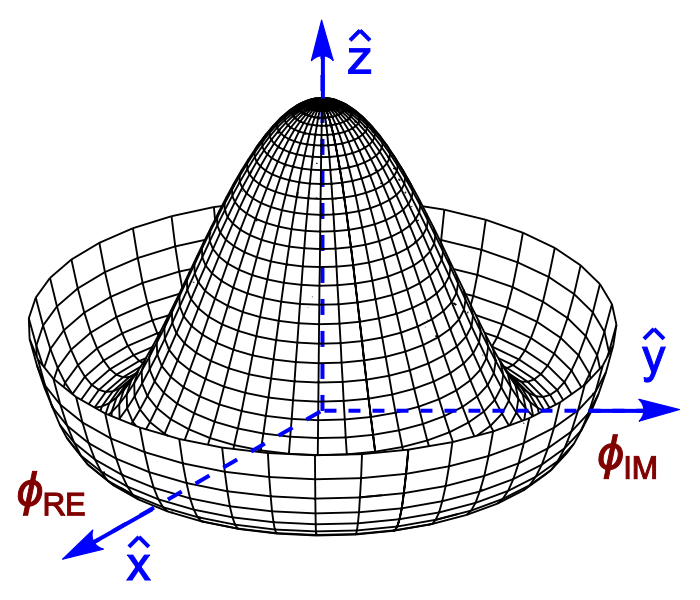
\includegraphics[width=.9\linewidth]{sombrero_potential}
\end{figure}

The terms in the Lagrangian \Cref{eq:ew_lagr} proportional to $\mu^2$ and $\lambda$ make up the ``Higgs potential''~\cite{Higgs:1964pj}.
We restrict $\lambda > 0$ to guarantee our potential is bounded from below, and we also require $\mu^2 < 0$, which gives us the standard ``sombrero'' potential shown in \Cref{fig:sombrero}.

This potential has infinitely many minima at $<\phi> = \sqrt{2m/\lambda}$.
The ground state is \textit{spontaneously} broken by the choice of ground state, which induces a vacuum expectation value (VEV).
Without loss of generality, we can choose the Higgs field $\phi$ to point in the real direction, and write the Higgs field $\phi$ in the following form:
\begin{equation}
\phi = \frac{1}{\sqrt{2}} \exp( \frac{i}{v} \sigma_a \theta_a ) \begin{pmatrix} 0 \\ v + h(x) \end{pmatrix}.
\end{equation}
We choose a gauge to rotate away the dependence on $\theta_a$, such that we can write simply
\begin{equation}
\label{eq:higgs_field_after_ssb}
\phi = \frac{1}{\sqrt{2}} \begin{pmatrix} 0 \\ v + h(x) \end{pmatrix}.
\end{equation}
Now, we see how the masses of the vector bosons are generated from the application of the Higgs mechanism.
We plug \Cref{eq:higgs_field_after_ssb} back into the electroweak Lagrangian, and only showing the relevant mass terms in the vacuum state where $h(x) = 0$  see that (dropping the Lorentz indices) :
\begin{align}
\Lagr_M = \frac{1}{8} \begin{vmatrix} \begin{pmatrix} gW_3 + g'B & g(W_1 - iW_2)\\ g(W_1 + iW_2) & -gW_3 + g'B \end{pmatrix}  \begin{pmatrix} 0  \\ v \end{pmatrix} \end{vmatrix}^2\\ = \frac{g^2 v^2}{8} \begin{bmatrix} W_1^2 + W_2^2 + (\frac{g'}{g}B - W_3)^2 \end{bmatrix} \notag
\end{align}
Defining the \textit{Weinberg} angle $\tan(\theta_W) = g'/g$ and the following \textit{physical} fields :
\begin{align}
W^{\pm} &= \frac{1}{\sqrt{2}}(W_1 \mp iW_2) \\
Z^0 &= \cos \theta_W W_3 - \sin\theta_W B \notag\\
A^0 &= \sin \theta_W W_3 + \cos\theta_W B \notag
\end{align}
we can write the piece of the Lagrangian associated to the vector boson masses as
\begin{equation}
\Lagr_{M_V} = \frac{1}{4} g^2 v^2 W^+ W^- + \frac{1}{8} (g^2 + g'^2)v^2 Z^0 Z^0 .
\end{equation}
We have the following values of the masses for the vector bosons :
\begin{align}
m_W^2 &= \frac{1}{4}  v^2 g^2  \\
m_Z^2 &= \frac{1}{4}  v^2 (g^2 + g'^2)  \notag \\
m_A^2 &= 0  \notag
\end{align}
We thus see how the Higgs mechanism gives rise to the masses of the $W^{\pm}$ and $Z$ boson in the Standard Model.
As expected, the mass of the photon is zero.
The $SU(2)_L \otimes U(1)_Y$ symmetry of the initially massless $W_{1,2,3}$ and $B$ fields is broken to the $U(1)_{EM}$.
Of the four degrees of freedom in the complex Higgs doublet, three are ``eaten'' to give mass to the $W^\pm$ and $Z^0$, while the other degree of freedom is the Higgs particle, as discovered in 2012 by the ATLAS and CMS collaborations~\cite{HIGG-2012-27, CMS-HIG-12-028}.

\subsection{Quantum Chromodynamics}

Quantum chromodynamics (or the theory of the \textit{strong} force) characterizes the behavior of \textit{colored} particles, collectively known as \textit{partons}.
The partons of the Standard Model are the (fermionic) quarks, and the (bosonic) gluons.
The strong force is governed by $SU(3)_C$, an unbroken symmetry in the Standard Model, which implies the gluon remains massless.
Defining the covariant derivative for QCD as
\begin{align}
\Dmuup = \dmuup + ig_s G^\mu_a L_a, a = 1,...,8
\end{align}
where $L_a$ are the generators of $SU(3)_C$, and $g_s$ is the coupling constant of the strong force.
The QCD Lagrangian then is given by
\begin{equation}
\Lagr_{\text{QCD}} = i \bar{\psi}_f \Dmu \gamma^\mu \psi_f - \frac{1}{4} G_{a,\mu\nu} G_a^{\mu\nu}
\end{equation}
where the summation over $f$ is for quarks \textit{families}, and $ G_a^{\mu\nu}$ is the gluon field strength tensor, given by
\begin{equation}
G^{\mu\nu}_a = \dmuup G^\nu_a - \partial^\nu G^\mu_a - g_s f^{abc} G^\mu_b G^\nu_c, \xspace a,b,c = 1,...,8
\end{equation}
where $f^{abc}$ are the structure constants of $SU(3)_C$, which are analogous to $\epsilon_{abc}$ for $SU(2)_L$.
The kinetic term for the quarks is contained in the $\dmu$ term, while the field strength term contains the interactions between the quarks and gluons, as well as the gluon self-interactions.

Written down in this simple form, the QCD Lagrangian does not seem much different from the QED Lagrangian, with the proper adjustments for the different group structures.
The gluon is massless, like the photon, so one could n\"aively expect an infinite range force, and it pays to understand why this is not the case.
The reason for this fundamental difference is the gluon self-interactions  arising in the field strength tensor term of the Lagrangian.
This leads to the phenomena of \textit{color confinement}, which describes why we only observe color-neutral particles alone in nature.
In contrast to the electromagnetic force, particles which interact via the strong force experience a \textit{greater} force as the distance between the particles increases.
At long distances, the potential is given by $V(r) = -kr$.
At some point, it is more energetically favorable to create additional partons out of the vacuum than continue pulling apart the existing partons, and the colored particles undergo \textit{fragmentation}.
This leads to \textit{hadronization}.
Bare quarks and gluons are actually observed as sprays of hadrons (primarily kaons and pions).
These sprays are known as \textit{jets}, which are what are observed by experiments.

\begin{sidewaysfigure}[htbp]
%\begin{figure}[tbp][hptb]
\caption{Cross-sections of various Standard Model processes as measured by ATLAS}
\label{fig:sm_xsec}
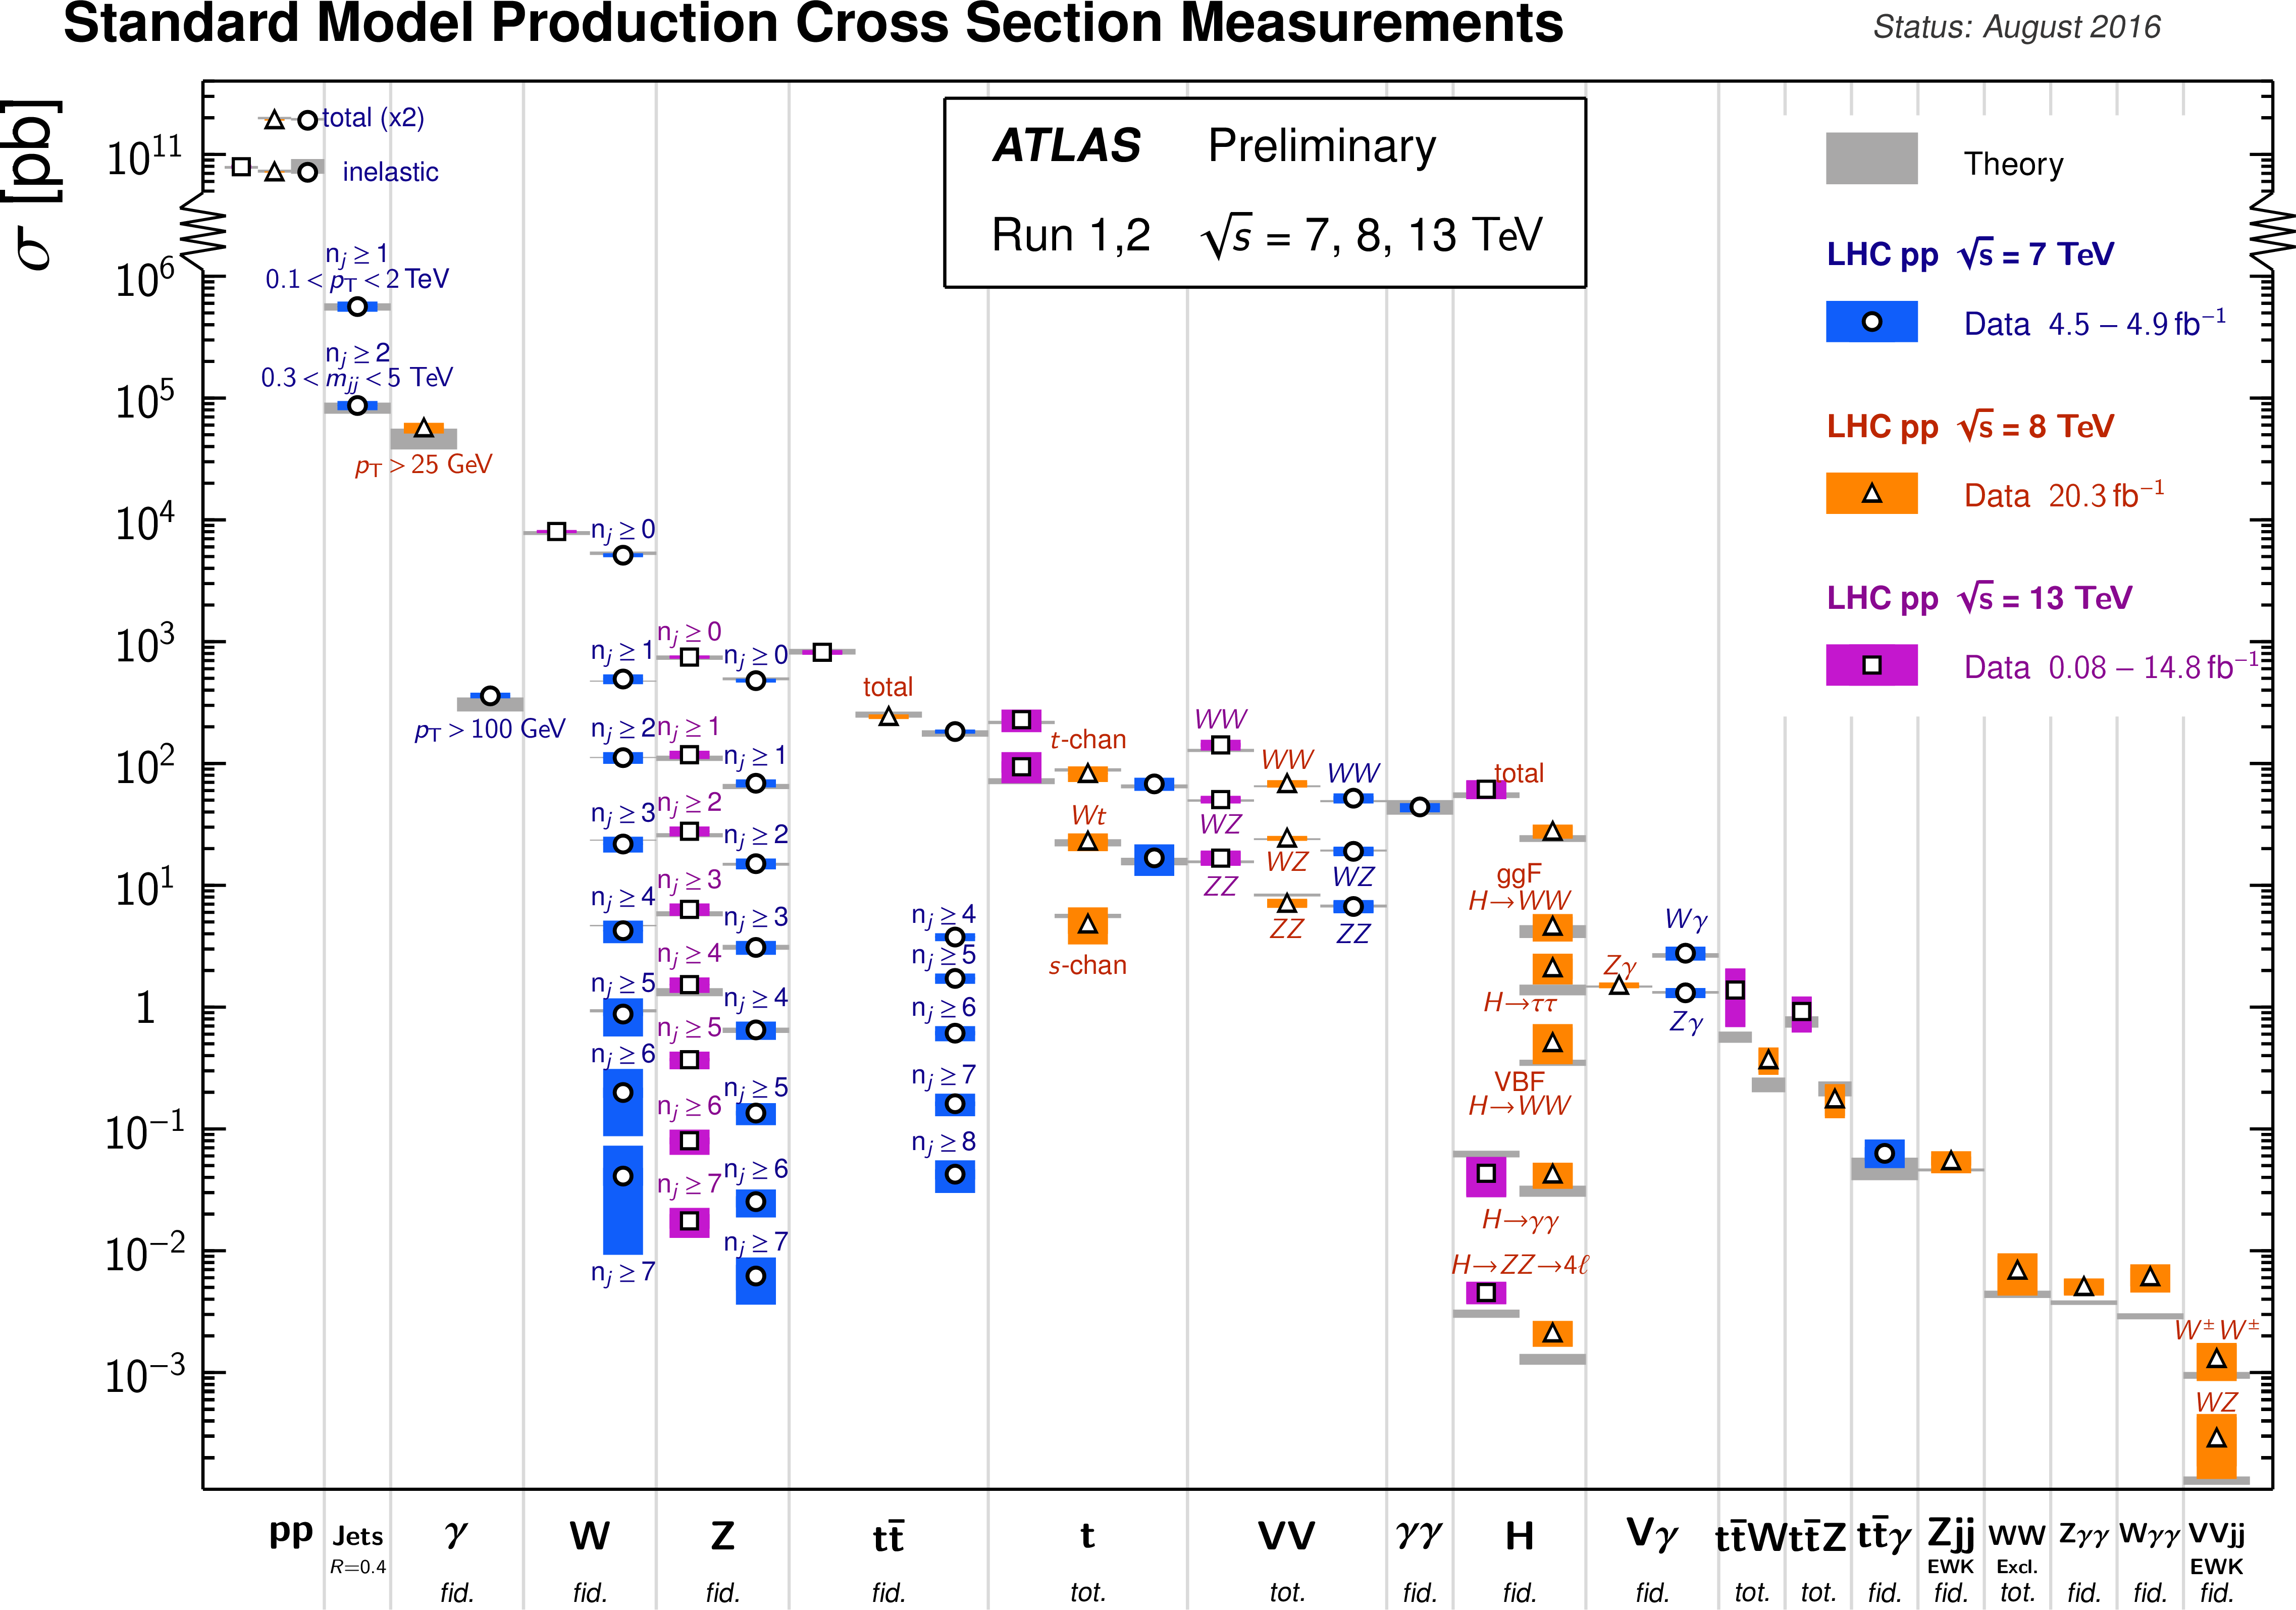
\includegraphics[width=.9\linewidth]{ATLAS_b_SMSummary_FiducialXsect}
\end{sidewaysfigure}

It is important to recognize the importance of understanding these QCD interactions in high-energy hadron colliders such as the LHC.
Since protons are hadrons, proton-proton collisions such as those produced by the LHC are primarily governed by the processes of QCD.
In particular, by far the most frequent process observed in LHC experiments is dijet production from gluon-gluon interactions; see \Cref{fig:sm_xsec}).
The interacting gluons are part of the \textit{sea} inside the proton; the simple $p = uud$ model does not apply.
The main \textit{valence} $uud$ quarks are constantly interacting via gluons, which can themselves radiate gluons or split into quarks, and so on.
A more useful understanding is given by the colloquially-known \textit{bag} model~\cite{Chodos:1974je, Chodos:1974pn}, where the proton is seen as a ``bag'' of (in principle) infinitely many partons, each with energy $ E < \sqrt{s} = 6.5 \TeV$.
One then collides this (proton) bag with another, and views the products of this very complicated collision, where calculations include many loops in nonperturbative QCD calculations.

Fortunately, we are generally saved by the QCD factorization theorems~\cite{Collins:1989gx}.
This allows one to understand the hard (i.e. short distance or high energy) $2 \rightarrow 2$ parton process using the tools of perturbative QCD, while making series of approximations known as a \textit{parton shower} model to understand the additional corrections from nonpertubative QCD.
We will discuss the reconstruction of jets by experiments in \Cref{ch:reconstruction}.

\subsection{Fermions}

We will now look more closely at the fermions in the Standard Model~\cite{Agashe:2014kda}.

As noted earlier in \Cref{sec:field_content}, the fermions of the Standard Model can be first distinguished between those that interact via the strong force (quarks) and those which do not (leptons).

There are six leptons in the Standard Model, which can be placed into three \textit{generations}.
\begin{equation}
\begin{pmatrix} e \\ \nu_e \end{pmatrix} , \begin{pmatrix} \mu \\ \nu_\mu \end{pmatrix}, \begin{pmatrix} \tau \\ \nu_\tau \end{pmatrix}
\end{equation}
There is the electron ($e)$, muon ($\mu$), and tau ($\tau$), each of which has an associated neutrino ($\nu_e, \nu_\mu, \nu_\tau$).
Each of the so-called charged (``electron-like'') leptons has electromagnetic charge $-1$, while the neutrinos all have $q_{EM} = 0$.

Often in an experimental context, lepton is used to denote the stable electron and metastable muon, due to their striking experimental signatures.
Taus are often treated separately, due to their much shorter lifetime of $\tau_{\tau} \order 10^{-13}$ s.
They decay through hadrons or the other leptons, so often physics analyses at the LHC treat them as jets or leptons, as will be done in this thesis.

As the neutrinos are electrically neutral, nearly massless, and only interact via the weak force, it is quite difficult to observe them directly.
Since LHC experiments rely overwhelmingly on electromagnetic interactions to observe particles, the presence of neutrinos is not observed directly.
Neutrinos are instead observed by the conservation of four-momentum in the plane transverse to the proton-proton collisions, known as \textit{missing transverse energy}.

There are six quarks in the Standard Model : up, down, charm, strange, top, and bottom.
Quarks are similar organized into three generations:
\begin{equation}
\begin{pmatrix} u \\ d \end{pmatrix} , \begin{pmatrix} c \\ s \end{pmatrix}, \begin{pmatrix} t \\ b \end{pmatrix}
\end{equation}
where we speak of ``up-like'' quarks and ``down-like'' quarks.

Each up-like quark has charge $q_{up} = 2/3$, while the down-like quarks have $q_{down} = -1/3$.
At the high energies of the LHC, one often makes the distinction between the light quarks ($u,d,c,s$), the bottom quark, and top quark.
In general, due to the hadronization process described above, the light quarks, with masses $m_q \undertilde{<} 1.5 \GeV$ are indistinguishable by LHC experiments.
Their hadronic decay products generally have long lifetimes and they are reconstructed as jets\footnotemark.
\footnotetext{In some contexts, charm quarks are also treated as a separate category, although it is quite difficult to distinguish charm quarks from the other light quarks at high energy colliders.}
The bottom quark hadronizes primarily through the $B$-mesons, which generally travels a short distance before decaying to other hadrons.
This allows one to distinguish decays via $b$-quarks from other jets.
This procedure is known as \textit{b-tagging} and will be discussed more in \Cref{Chapter-ATLAS}.

Due to its large mass, the top quark decays before it can hadronize.
There are no bound states associated to the top quark.
The top is of particular interest at the LHC; it has a striking signature through its most common decay mode $t \rightarrow Wb$.
Decays via tops, especially $\ttbar$, are frequently an important signal decay mode, or an important background process.

\subsection{Interactions in the Standard Model}
\begin{figure}[tbp]
\caption{The interactions of the Standard Model} \label{fig:sm_interactions}
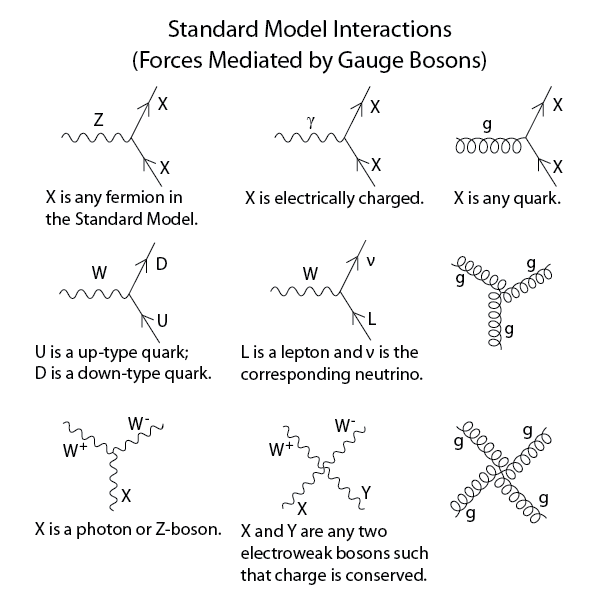
\includegraphics[width=.9\linewidth]{Standard_Model_Feynman_Diagram_Vertices}
\end{figure}

We briefly overview the entirety of the fundamental interactions of the Standard Model.
These can also be found in \Cref{fig:sm_interactions}.

The electromagnetic force, mediated by the photon, interacts via a three-point coupling with all charged particles in the Standard Model.
The photon thus interacts with all the quarks, the charged leptons, and the charged $W^\pm$ bosons.

The weak force is mediated by three particles: the $W^\pm$ and the $Z^0$.
The $Z^0$ can interacts with all fermions via a three-point coupling.
A real $Z^0$ can thus decay to a fermion-antifermion pair of all SM fermions except the top quark, due to its large mass.
The $W^\pm$ has two important three-point interactions with fermions.
First, the $W^\pm$ can interact with an up-like quark and a down-like quark; an important example in LHC experiments is $t \rightarrow Wb$.
The coupling constants for these interactions are encoded in the unitary matrix known as the Cabibbo–Kobayashi–Maskawa (CKM) matrix~\cite{Cabibbo:1963yz,Kobayashi:1973fv}, and are generally known as flavor-changing interactions.
Secondly, the $W^\pm$ interacts with a charged lepton and its corresponding neutrino.
In this case, the unitary matrix that corresponds to CKM matrix for quarks is the identity matrix, which forbids (fundamental) vertices such as $\mu \rightarrow We$.
For leptons, instead this is a two-step process: $\mu \rightarrow \nu_{\mu} W \rightarrow \nu_{\mu} \bar{\nu_e} e$.
Finally, there are the self-interactions of the weak gauge bosons.
There are three-point and four-point interactions.
All combinations are allowed which conserve electric charge.

The strong force is mediated by the gluon, which as discussed above also carries the strong color charge.
There is the fundamental three-point interaction, where a quark radiates a gluon.
Additionally, there are the three-point and four-point gluon self-interactions.

\section{Deficiencies of the Standard Model}
\label{sec:def_sm}

The Standard Model has been enormously successful.
This relatively simple theory is capable of explaining a very wide range of phenomenon, which can be described as combinations of the nine diagrams shown in \Cref{fig:sm_interactions} at tree level.
Unfortunately, there are some unexplained problems with the Standard Model.
We cannot go through all of the issues in this thesis, but we will motivate the primary issues which naturally lead one to \textit{supersymmetry}, as we will see in \Cref{ch:susy}.

The Standard Model has many free parameters, shown in \Cref{tab:sm_free_parameters}.
\begin{table}
\centering
\caption{Parameters of the Standard Model.  For values dependent on the renormalization scheme, we use a combination of the on-shell normalization scheme~\cite{Hollik:1988ii, Bardin:1989vz, Kennedy:1988rt, Sirlin:1980nh} and  modified minimal subtraction scheme with $m_{\bar{MS}}$ as indicated in the table~\cite{ Fanchiotti:1992tu}}.
\label{tab:sm_free_parameters}
\begin{tabular}{| l | l | l |}
\hline
$m_e$             & Electron mass                  & 511 keV                           \\ \hline
$m_\mu$           & Muon mass                      & 105.7 MeV                         \\ \hline
$m_\tau$          & Tau mass                       & 1.78 GeV                          \\ \hline
$m_u$             & Up quark mass                  & 1.9 MeV   ($m_{\bar{MS}} = 2 GeV$)                        \\ \hline
$m_d$             & Down quark mass                & 4.4 MeV   ($m_{\bar{MS}} = 2 GeV$)                       \\ \hline
$m_s$             & Strange quark mass             & 87 MeV    ($m_{\bar{MS}} = 2 GeV$)                        \\ \hline
$m_c$             & Charm quark mass               & 1.32 GeV  ($m_{\bar{MS}} = m_c$)                        \\ \hline
$m_b$             & Bottom quark mass              & 4.24 GeV  ($m_{\bar{MS}} = m_b$)  \\ \hline
$m_t$             & Top quark mass                 & 172.7 GeV (on-shell renormalization)                       \\ \hline
$\theta_{12}$ CKM & 12-mixing angle                & 13.1$^{\circ}$                    \\ \hline
$\theta_{23}$ CKM & 23-mixing angle                & 2.4$^{\circ}$                     \\ \hline
$\theta_{13}$ CKM & 13-mixing angle                & 0.2$^{\circ}$                     \\ \hline
$\delta$ CKM      & CP-violating Phase             & 0.995                             \\ \hline
$g'$              & U(1) gauge coupling            & 0.357     ($m_{\bar{MS}} = m_Z$)                         \\ \hline
$g$               & SU(2) gauge coupling           & 0.652     ($m_{\bar{MS}} = m_Z$)                         \\ \hline
$g_s$             & SU(3) gauge coupling           & 1.221     ($m_{\bar{MS}} = m_Z$)                         \\ \hline
$\theta{QCD}$     & QCD vacuum angle               & \order 0                          \\ \hline
VEV               & Higgs vacuum expectation value & 246 GeV                           \\ \hline
$m_H$             & Higgs mass                     & 125 GeV                           \\ \hline
\end{tabular}
\end{table}
In general, we prefer models with less free parameters.
A great example of this fact, and the primary experimental evidence for EWSB, is the relationship between the couplings of the weak force and the masses of the gauge bosons of the weak force:
\begin{equation}
\rho \equiv \frac{m_W^2}{m_Z^2 \cos^2 \theta_W } \stackrel{?}{=} 1
\end{equation}
where $?$ indicates that this is a testable prediction of the Standard Model (in particular, that the gauge bosons gain mass through EWSB).
This relationship has been measured  within experimental and theoretical predictions.
We would like to produce additional such relationships, which could exist if the Standard Model is a low-energy approximation of some other theory.

An additional issue is the lack of \textit{gauge coupling unification}.
The couplings of any quantum field theory ``run'' as a function of the distance scales (or inversely, energy scales) of the theory.
The idea is closely related to the unification of the electromagnetic and weak forces at the so-called \textit{electroweak scale} of $O(100 \GeV)$.
One would hope this behavior was repeated between the electroweak forces and the strong force at some suitable energy scale.
\begin{figure}[tbp]
\caption{The running of Standard Model gauge couplings.  The Standard Model couplings do not unify at high energies, which indicates it cannot completely describe nature through the Planck scale.} \label{fig:sm_gauge_coupling}
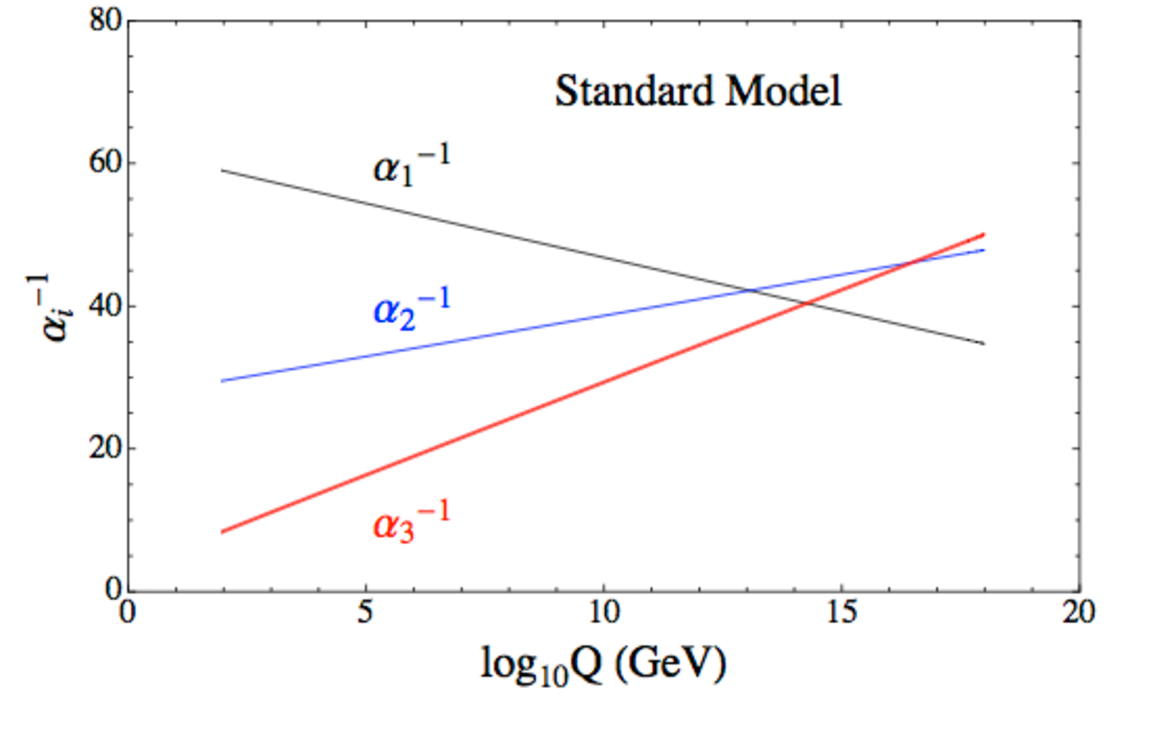
\includegraphics[width=.9\linewidth]{Grand_unification_couplings_sm}
\end{figure}
The Standard Model does not exhibit this behavior, as we can see in \Cref{fig:sm_gauge_coupling}.

\begin{figure}[tbp]
\caption{The dominant quantum loop correction to the Higgs mass in the Standard Model} \label{fig:sm_higgs_corrections}
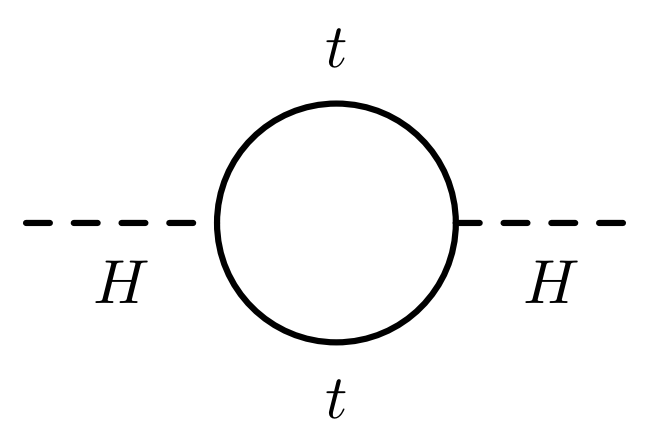
\includegraphics[width=.9\linewidth]{sm_higgs_corrections}
\end{figure}
But, the most significant problem with the Standard Model is the \textit{hierarchy problem}.
In its most straightforward incarnation, the Higgs scalar field is subject to quantum corrections through loop diagrams, as shown in \Cref{fig:sm_higgs_corrections}.
For demonstration, we use the contributions from the top quark, since the top quark has the largest Higgs Yukawa coupling due to its large mass.
In general, we should expect these corrections to quadratically dependent on the scale of the ultraviolet physics, $\Lambda$.
Briefly assume there is no new physics before the Planck scale of gravity, $\Lambda_{\text{Planck}} = 10^{19} \GeV$.
In this case, we expect the corrections to the Higgs mass to be
\begin{equation}
\delta m^2_H \approx \Big( \frac{m_t}{8\pi^2 <\phi>_{VEV}} \Big)^2 \Lambda_{Planck}^2.
\end{equation}
To achieve the miraculous cancellation required to get the observed Higgs mass of 125 \GeV, one needs to then set the bare Higgs mass $m_0$, our input to the Standard Model Lagrangian, itself to a \textit{precise} value $\order 10^{19} \GeV$.
This extraordinary level of parameter finetuning is quite undesirable, and within the framework of the Standard Model alone, there is little that can be done to alleviate this issue.

An additional concern, of a different nature, is the lack of a \textit{dark matter} candidate in the Standard Model.
Dark matter was discovered by observing galactic rotation curves, which showed that much of the matter that interacts gravitionally is invisible to our (electromagnetic) telescopes~\cite{Rubin:1970zza, Roberts:1970zza, Rubin:1980zd, Rubin:1985ze, Bosma:1981zz, Persic:1995ru, darkMatterPrimer}.
The postulation of the existence of dark matter, which interacts at least through gravity, allows one to understand these galatic rotation curves.
Unfortunately, no particle in the Standard Model could possibly be the dark matter particle.
The only candidate truly worth another look is the neutrino, but it has been shown that the neutrino content of the universe is simply too small to explain the galatic rotation curves~\cite{Quigg:2008ab, darkMatterPrimer}.
The experimental evidence from the galactic rotations curves thus show there \textit{must} be additional physics beyond the Standard Model which is yet to be understood.

In the next chapter, we will see how these problems can be alleviated by the theory of supersymmetry.

\begin{figure}[tbp]
\caption{Particles of the Standard Model} \label{fig:sm_particles}
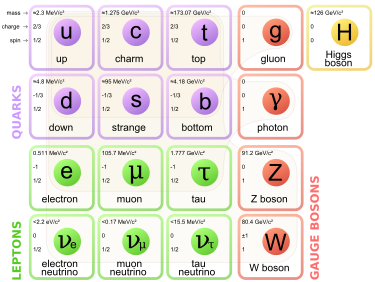
\includegraphics[width=.9\linewidth]{Standard_Model_of_Elementary_Particles}
\end{figure}

% \subsection{$\Lagr_{\psi}$ }

% We cannot write down any mass terms for fermions in the Standard Model.
% Dirac mass terms are forbidden since they are all assigned to ``chiral'' representations of the gauge symmetry.
% Majorana mass terms are disallowed since there are no fields with $Y \slashed{=} 0$.

% \subsection{$\Lagr_{Yuk}$ }

% We write the Yukawa portion of the Standard Model Lagrangian

% \begin{equation}
% \Lagr_{Yuk} = Y_{ij}\bar{L_{Li} E_{Rj}} \phi + h.c.
% \end{equation}

% The Yukawa matrix $Y$ is a general complex 3 $\times$ 3 matrix of dimensionless couplings which can be diagonalized, leading to a diagonal matrix with only three real parameters $(y_e , y_\mu , y_\tau)$.
% This reflects the fact that for the electron, muon, and tau lepton, the interaction basis is the same as the mass basis; this is the same as saying an electron has a well-defined mass.

% \section{$\Lagr_\phi$, Electroweak Symmetry breaking and the Higgs Boson}

% Let us now recall that local gauge invariance means that the vector fields in this theory are \textit{massless}.
% N\"aively, it seems this combined with the chirality of the Standard Model, that \textit{none} of the fields have masses.
% The solution to this seeming conundrum is of course the well-known ``Higgs'' mechanism, described in Sec. \Cref{subsec:symmetry_breaking}.

% In the Standard Model, the Higgs potential is given by
% \begin{equation} \label{eq:higgs_potential}
% \Lagr_\phi = -\mu^2 \phi^\dagger \phi - \lambda (\phi^\dagger \phi)^2.
% \end{equation}

% Since $\lambda$ is dimensionless and real, to have a potential bounded from below, we require $\lambda > 0$.
% To break the gauge symmetry, we require $\mu^2 < 0$, leading again to the sombrero potential \Cref{fig:sombrero}.
% We define
% \begin{equation}
% v^2 = - \frac{\mu^2}{\lambda}.
% \end{equation}

% This allows us to write \Cref{eq:higgs_potential} as
% \begin{equation} \label{eq:higgs_potential_rewritten}
% \Lagr_\phi = - \lambda (\phi^\dagger \phi - \frac{v^2}{2})^2
% \end{equation}
% after dropping the constant term.

% This means the $\phi$ field acquires a VEV $|<\phi>| = v/\sqrt{2}$.
% Choosing the convenient gauge
% \begin{equation}
% \phi = \begin{pmatrix} 0 \\ v/\sqrt{2} \end{pmatrix},
% \end{equation}

% The VEV breaks the $SU(2)_L \otimes U(1)_Y$ symmetry to a $U(1)_{EM}$ subgroup.
% We can identify the unbroken generator of this $U(1)_{EM}$ subgroup as $Q_{EM} = T_3 + Y/2$, since this vanishes in the down component
% \begin{equation}
% Q_{\gamma} \phi = (T_3 + Y/2) \phi = (\frac{1}{2} \sigmathree + \frac{1}{2} I ) \begin{pmatrix} 0 \\ v/\sqrt{2} \end{pmatrix}.
% \end{equation}
% Here we see the indicative $\gamma$ for the photon, as this unbroken $U(1)_{EM}$ symmetry is of course the symmetry associated to the electromagnetic force mediated by the gauge boson known as the photon.

% There are three broken generators: $T_1, T_2, T_3 - Y/2$.
% These are each associated to one of the massive gauge bosons induced by the symmetry breaking.
% Choosing a gauge which rotates away the ``eaten'' Goldstone boson degrees of freedom, we can write the Higgs field as
% \begin{equation}
% \label{eq:higgs_field}
% \phi = \frac{1}{\sqrt{2}}\begin{pmatrix} 0 \\ v + h(x) \end{pmatrix}.
% \end{equation}

% \section{Particle Spectrum: Standard Model Lagrangian after Electroweak Symmetry Breaking}

% We can now return to the Standard Model Lagrangian and use the equation for the Higgs field after EWSB \Cref{eq:higgs_field}.
% This will show us the ``physical'' particle content of the Standard Model.

% \subsection{Particle content associated to $\Lagr_\phi$}

% Setting $phi$ as in \Cref{eq:higgs_field}, we quickly see that we can rewrite \Cref{eq:higgs_potential_rewritten} as
% \begin{equation}
% \Lagr_\phi = - \lambda (\phi^\dagger \phi - \frac{v^2}{2})^2  = - \lambda ( \frac{1}{2} (v + h(x))^2 - \frac{v^2}{2})^2 = - \lambda ( h(x)^2 + vh(x))^2 = -\lambda ( h(x)^4 + v h(x)^3 + \frac{v^2}{2} h(x)^2 ).
% \end{equation}

% Interpreting the Higgs field squared term as the mass term of the Higgs boson, we see that $m_H = \sqrt{2 \lambda} v$.

% \subsection{Particle content associated to $\Lagr_{kin}$}

% Again using Eq.\Cref{eq:higgs_field} and $\Dmuup = \dmuup + ig_s G^\mu_a L_a + i g W^\mu_a T_a + i g' Y B^\mu $, we can see how the mass terms associated to the three massive gauge bosons, and also see how the photon stays massless.
% The mass terms for the gauge boson fields come from the kinetic term of the Higgs field:
% For each of the vector boson fields, we have the follow field strengths:

% \begin{equation}
% \begin{align}
% G^{\mu\nu}_a = \dmuup G^\nu_a + \partial^\nu G^\mu_a - g_s f_{abc} G^\mu_b G^\nu_c \\
% W^{\mu\nu}_a = \dmuup W^\nu_a + \partial^\nu W^\mu_a - g \epsilon_{abc} W_b^\mu W_c^\nu \\
% B^{\mu\nu}   = \dmuup B^\nu   + \partial^\nu B^\mu
% \end{align}
% \end{equation}

% where $g$ and $g_s$ are the electroweak and strong coupling constant.

% We can write the covariant derivative for the Standard Model as
% \begin{equation}
% \Dmuup = \dmuup + ig_s G^\mu_a L_a + i g W^\mu_a T_a + i g' Y B^\mu
% \end{equation}
% where $L_a$ and $T_a$ are the generators of $SU(3)_C $ and $SU(2)_L$ respectively for each of the representations.
% For $SU(2)_L$ doublets, $T_a = \frac{1}{2} \sigma_a $ and for $SU(2)_L$ singlets, $T_a = 0$.

% The combination of these terms allows us to write the kinetic terms of the Lagrangian as
% \begin{equation}
% \begin{align}
% \Lagr_{kin} = G^{\mu\nu} G_{\mu\nu} + W^{\mu\nu} W_{\mu\nu} + B^{\mu\nu} B_{\mu\nu}\\
%  + \Dmuup Q_L \Dmu Q_L + \Dmuup U_R \Dmu U_R +  \Dmuup D_R \Dmu D_R + \Dmuup L_L \Dmu L_LL + \Dmuup E_R \Dmu E_R
% \end{align}
% \end{equation}
%Recursive Jigsaw Reconstruction
%This is the first chapter of the dissertation

%The following command starts your chapter. If you want different titles used in your ToC and at the top of the page throughout the chapter, you can specify those values here. Since Columbia doesn't want extra information in the headers and footers, the "Top of Page Title" value won't actually appear.

\chapter[Supersymmetry][Top of Page Title]{Supersymmetry}\label{ch:susy}

Here you can write some introductory remarks about your chapter.
I like to give each sentence its own line.

When you need a new paragraph, just skip an extra line.

\section{Motivation}

\subsection{Only Additional allowed Lorentz invariant symmetry}
\subsection{Dark Matter}
\subsection{Cancellation of quadratic divergences in corrections to the Higgs Mass}

\section{Supersymmetry}

\section{Additional particle content}

\section{Phenomenology}

R parity
Consequences for sq/gl decays
%Search for SUSY in events with 0L using RJR
%This is the first chapter of the dissertation

%The following command starts your chapter. If you want different titles used in your ToC and at the top of the page throughout the chapter, you can specify those values here. Since Columbia doesn't want extra information in the headers and footers, the "Top of Page Title" value won't actually appear.

\chapter[Table of Contents Title][Top of Page Title]{Title of Chapter 1}

Here you can write some introductory remarks about your chapter.
I like to give each sentence its own line.

When you need a new paragraph, just skip an extra line.

\section*{New Section}

By using the asterisk to start a new section, I keep the section from appearing in the table of contents.
If you want your sections to be numbered and to appear in the table of contents, remove the asterisk.

%SUSY theory
%This is the first chapter of the dissertation

%The following command starts your chapter. If you want different titles used in your ToC and at the top of the page throughout the chapter, you can specify those values here. Since Columbia doesn't want extra information in the headers and footers, the "Top of Page Title" value won't actually appear.

\chapter[Table of Contents Title][Top of Page Title]{Title of Chapter 1}

Here you can write some introductory remarks about your chapter.
I like to give each sentence its own line.

When you need a new paragraph, just skip an extra line.

\section*{New Section}

By using the asterisk to start a new section, I keep the section from appearing in the table of contents.
If you want your sections to be numbered and to appear in the table of contents, remove the asterisk.

%SUSY theory
%This is the first chapter of the dissertation

%The following command starts your chapter. If you want different titles used in your ToC and at the top of the page throughout the chapter, you can specify those values here. Since Columbia doesn't want extra information in the headers and footers, the "Top of Page Title" value won't actually appear.

\chapter[Event Reconstruction][Top of Page Title]{Event Reconstruction}

This chapter describes the reconstruction algorithms used within ATLAS.\todo{cite fermilab lectures}
We will make the distinction between the ``primitive'' objects which are reconstructed from the detector signals from the ``composite'' physics objects we use in measurements and searches for new physics.

\section{Primitive Object Reconstruction}

The primitive objects reconstructed by ATLAS are \textit{tracks} and (calorimeter) \textit{clusters}.
These are reconstructed directly from tracking hits and calorimeter energy deposits into cells.
Tracks can be further divided into inner detector and muon spectrometer tracks.
Calorimeter clusters can be divided into sliding-window clusters and topological clusters (topoclusters).
% \footnotemark
% \footnotetext{Strictly speaking, sliding-window and topological clustering are the names of the algorithms, and thus one could speak of topological electromagnetic clusters or hadronic sliding-window clusters.
% In ATLAS, sliding-window is almost exclusively used to reconstruct electromagnetic objects and topological clustering is almost exclusively used for hadronic clustering, so to avoid confusion we will use this terminology here.
% These choices are entirely based on optimizing the object reconstruction efficiency relative to the fake rate.
% }
\subsection{Inner Detector Tracks}\label{sec:id_tracks}
\todo{cite paper/note}

Inner detector tracks are reconstructed from hits in the inner detector.
These hits indicate that a charged particle has passed through the detector material.
Due to the 2 T solenoid in the inner detector, the hits associated with any individual particle will be curved; this allows one to measure the momentum of the particle.
In any given event, there is upwards of \todo{number}, making it impossible to do any sort of combinatorics to reconstruct tracks\footnotemark.
There are two algorithms used by ATLAS track reconstruction, known as \textit{inside-out} and \textit{outside-in}.

ATLAS first employs the inside-out algorithm.
First, one assumes the track begins at the interaction point.
Moving out from the interaction point, one creates track seeds.
Track seeds are proto-tracks constructed from three hits; these hits can be distributed as three pixel hits, two pixel hits and one SCT hit, or three SCT hits.
One extrapolates the track and uses a combinatorial Kalman filter \todo{cite}, which adds the rest of the pixel and SCT hits to the seeds.
This is done seed by seed, so it avoids the combinatorial complexity involved with checking all hits with all seeds.
At this point, the algorithm applies an additional filter to avoid ambiguities from nearby tracks.
The TRT hits are then added to the seeds in the same procedure; in this way, all hits are associated to a track.

The next step is to figure out the correct kinematics of the track.
This is done by applying a fitting algorithm which outputs the best-fit track parameters by minimizing the track distance from hits, weighted by each hit's resolution.
These parameters are $(d_0, z_0, \eta, \phi, q/p)$ where $d_0$ ($z_0$) is the transverse (longitudinal) impact parameter and $q/p$ is the charge over the track momenta.
This set of parameters uniquely defines the trajectory of the charged particle associated to the track; an illustration of a track with these parameters is shown in Fig.\ref{fig:track_schematic}.

\begin{figure}
\caption{The parameters associated to a track.}
\label{fig:track_schematic}
\includegraphics[width=.45\linewidth]{track_schematic}
\end{figure}

The other track reconstruction algorithm is the outside-in algorithm.
As the name implies, in this case, we start from the outside of the inner detector, in the TRT, and extend the tracks in.
One begins by seeding from TRT hits, and extending the track back towards the center of the detector.
The same fitting procedure is used as in the inside-out algorithm to find the optimal track parameters.
This algorithm is particularly important for finding tracks which originate from interactions with the detector material, especially the SCT.
For tracks from primary vertices, this often finds the same tracks as the inside-out algorithm, providing an important check on the consistency of the tracking procedure.

In the high lumonosity environment of the LHC, even the tracks reconstructed from precision detectors such as those of ATLAS inner detector can sometimes lead to fake tracks from simple combinatoric chance.
Several quality checks are imposed after track fitting which reduce this background.
Seven silicon (pixel + SCT) hits are required for all tracks.
No more than two holes are allowed in the pixel detector; holes are expected measurements from the track that are missing in the pixel detector.
Finally, tracks with poor fit quality, as measured by $\chi^2/ndf$, are also rejected.
Due to the high quality of the silicon measurements in the pixel detector and SCT, these requirements give good track reconstruction efficiency, as seen in Fig.\ref{fig:track_eff} for simulated events\cite{ATL-COM-PHYS-2012-1541}.
\begin{figure}
\caption{Track reconstruction efficiency as a function of track \pt and $\eta$.
The efficiency is defined as the number of reconstructed tracks divided by the number of generate charged particles.} \label{fig:track_eff}
\subfloat[Track reconstruction as a function of \pt.]   {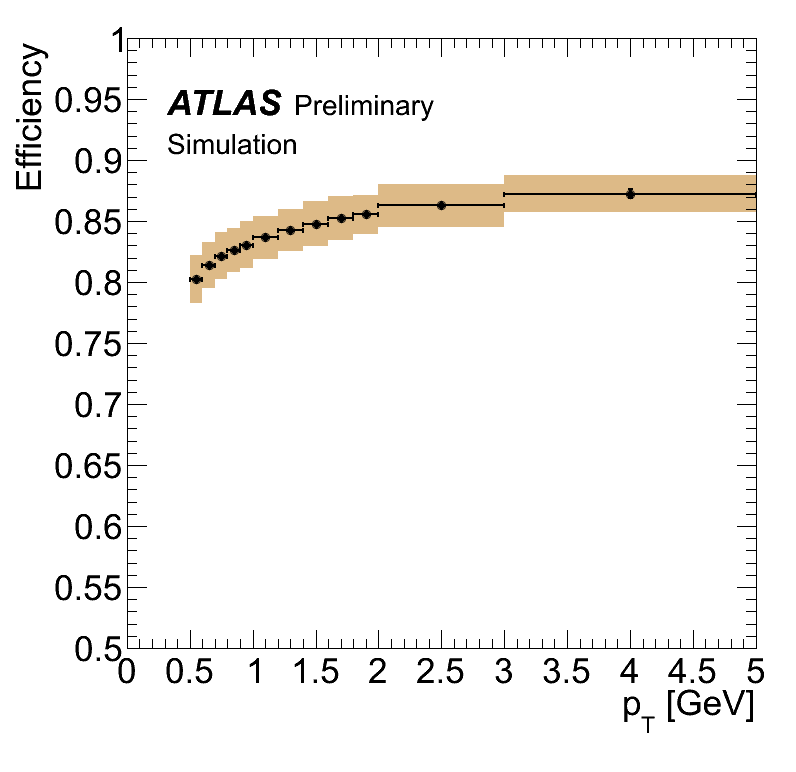
\includegraphics[width=.45\linewidth]{track_eff_pt}}
\subfloat[Track reconstruction as a function of $\eta$.]{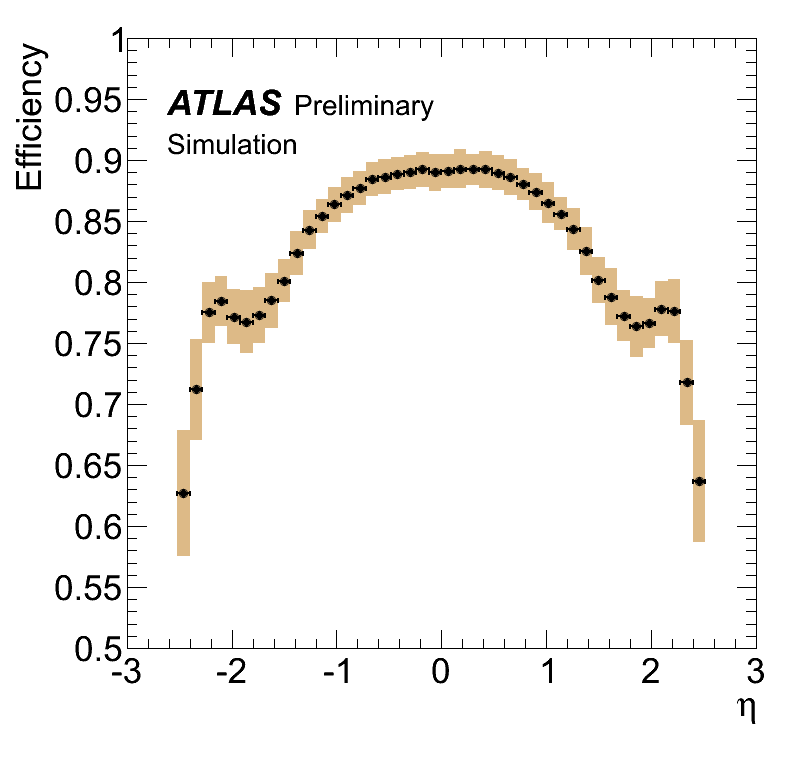
\includegraphics[width=.45\linewidth]{track_eff_eta}} \\
\end{figure}

\subsection{Sliding-window clusters}\label{sec:sliding_window_cluster}

The sliding-window algorithm is a way to combine calorimeter cells into composite objects (clusters) to be used as inputs for other algorithms\cite{PERF-2013-03}.
Sliding-window clusters are the primary inputs to electron and photon reconstruction, as described below.
As described in Ch.\ref{ch:atlas}, the electromagnetic calorimeter has high granularity, with a cell size of $(\eta, \phi) = (.025, .025)$ in the coarsest second layer throughout most of the calorimeter.
The ``window'' consists of 3 by 5 cells in the $(\eta, \phi)$ space; all layers are added on this same 2D space.
One translates this window over the space and seeds a cluster whenever the energy sum of the cells is maximized.
If the seed energy is greater than 2.5 \GeV, this seed is called a sliding-window cluster.
This choice was motivated to optimize the reconstruction efficiency of proto-electrons and proto-photons while rejecting fakes from electronic noise and additional particles from pileup vertices.

\subsection{Topological clusters}\label{sec:topoclusters}

Topoclusters are the output of the algorithm used within ATLAS to combine hadronic and electromagnetic calorimeter cells in a way which extracts signal from a background of significant electronic noise\cite{PERF-2014-07}.
They are the primary input to the algorithms which reconstruct jets.

Topological clusters are reconstructed from calorimeter cells in the following way.
First, one maps all cells onto a single $\eta-\phi$ plane so one can speak of \textit{neighboring} cells.
Two cells are considered neighboring if they are in the same layer and directly adjacent, or if they are in adjacent layers and overlap in $\eta-\phi$ space.
The \textit{significance} $\xi_{\text{cell}}$ of a cell during a given event is

\begin{equation}
\calosig = \frac{E_{\text{cell}}}{\sigma_{\text{noise,cell}}}
\end{equation}

where $\sigma_{\text{noise,cell}}$ is measured for each cell in ATLAS and $E_{\text{cell}}$ measures the current energy level of the cell.
One thinks of this as the measurement of the energy \textit{over threshold} for the cell.

Topocluster \textit{seeds} are defined as calorimeter cells which have a significance $\calosig > 4 $.
These are the inputs to the algorithm; one iteratively tests all cells adjacent to these seeds for $\calosig > 2$.
Each cells passing this selection is then added to the topocluster, and the procedure is repeated.
When the algorithm reaches the point where there are no additional adjacent cells with $\calosig > 2$, every positive-energy cell adjacent to the current proto-cluster is added.
This collection of cells is summed; the summed object is known as a topocluster.
An example of this procedure for a simulation dijet event is shown in Fig.\ref{fig:topocluster}.
\begin{figure}
\caption{Example of topoclustering on a simulated dijet event.} \label{fig:topocluster}
\subfloat[All cells with $\calosig > 4$.]{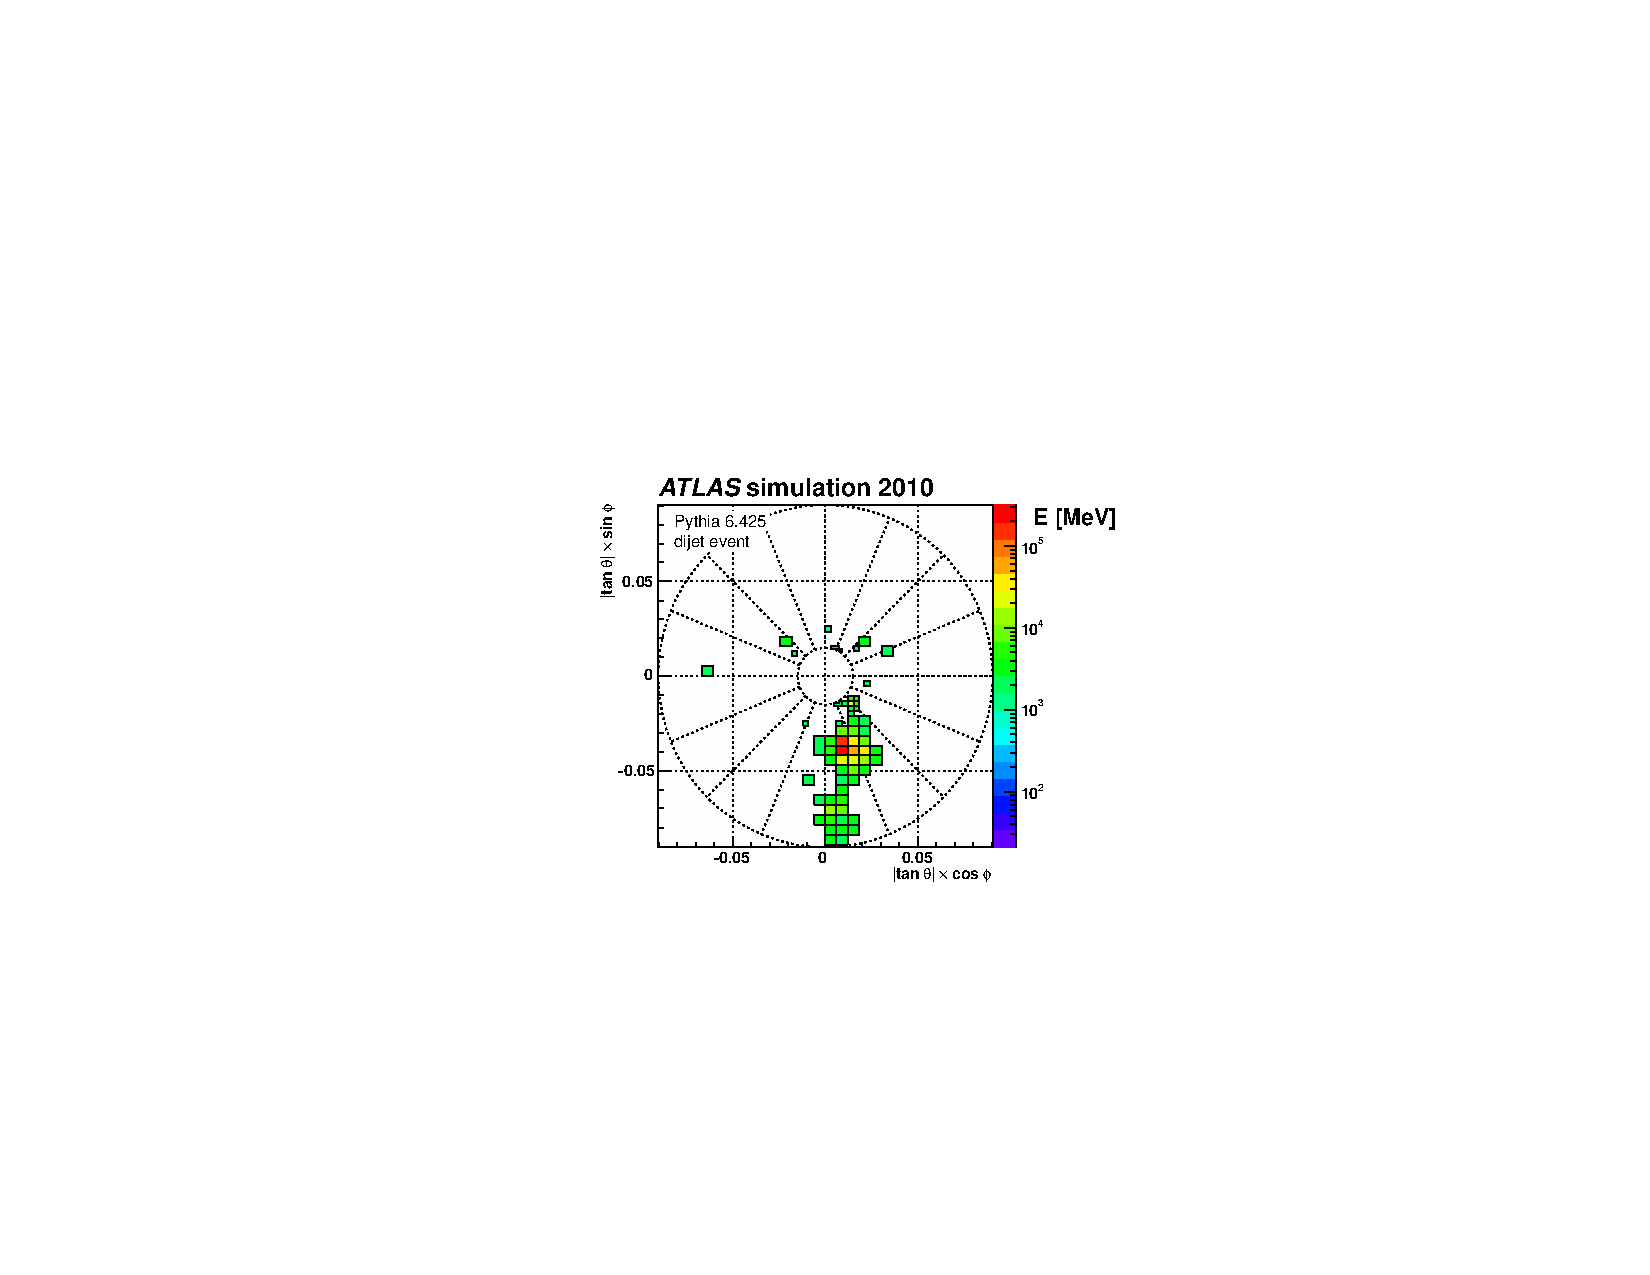
\includegraphics[width=.45\linewidth]{topoclustering_sig4.pdf}}
\subfloat[All cells with $\calosig > 2$.]{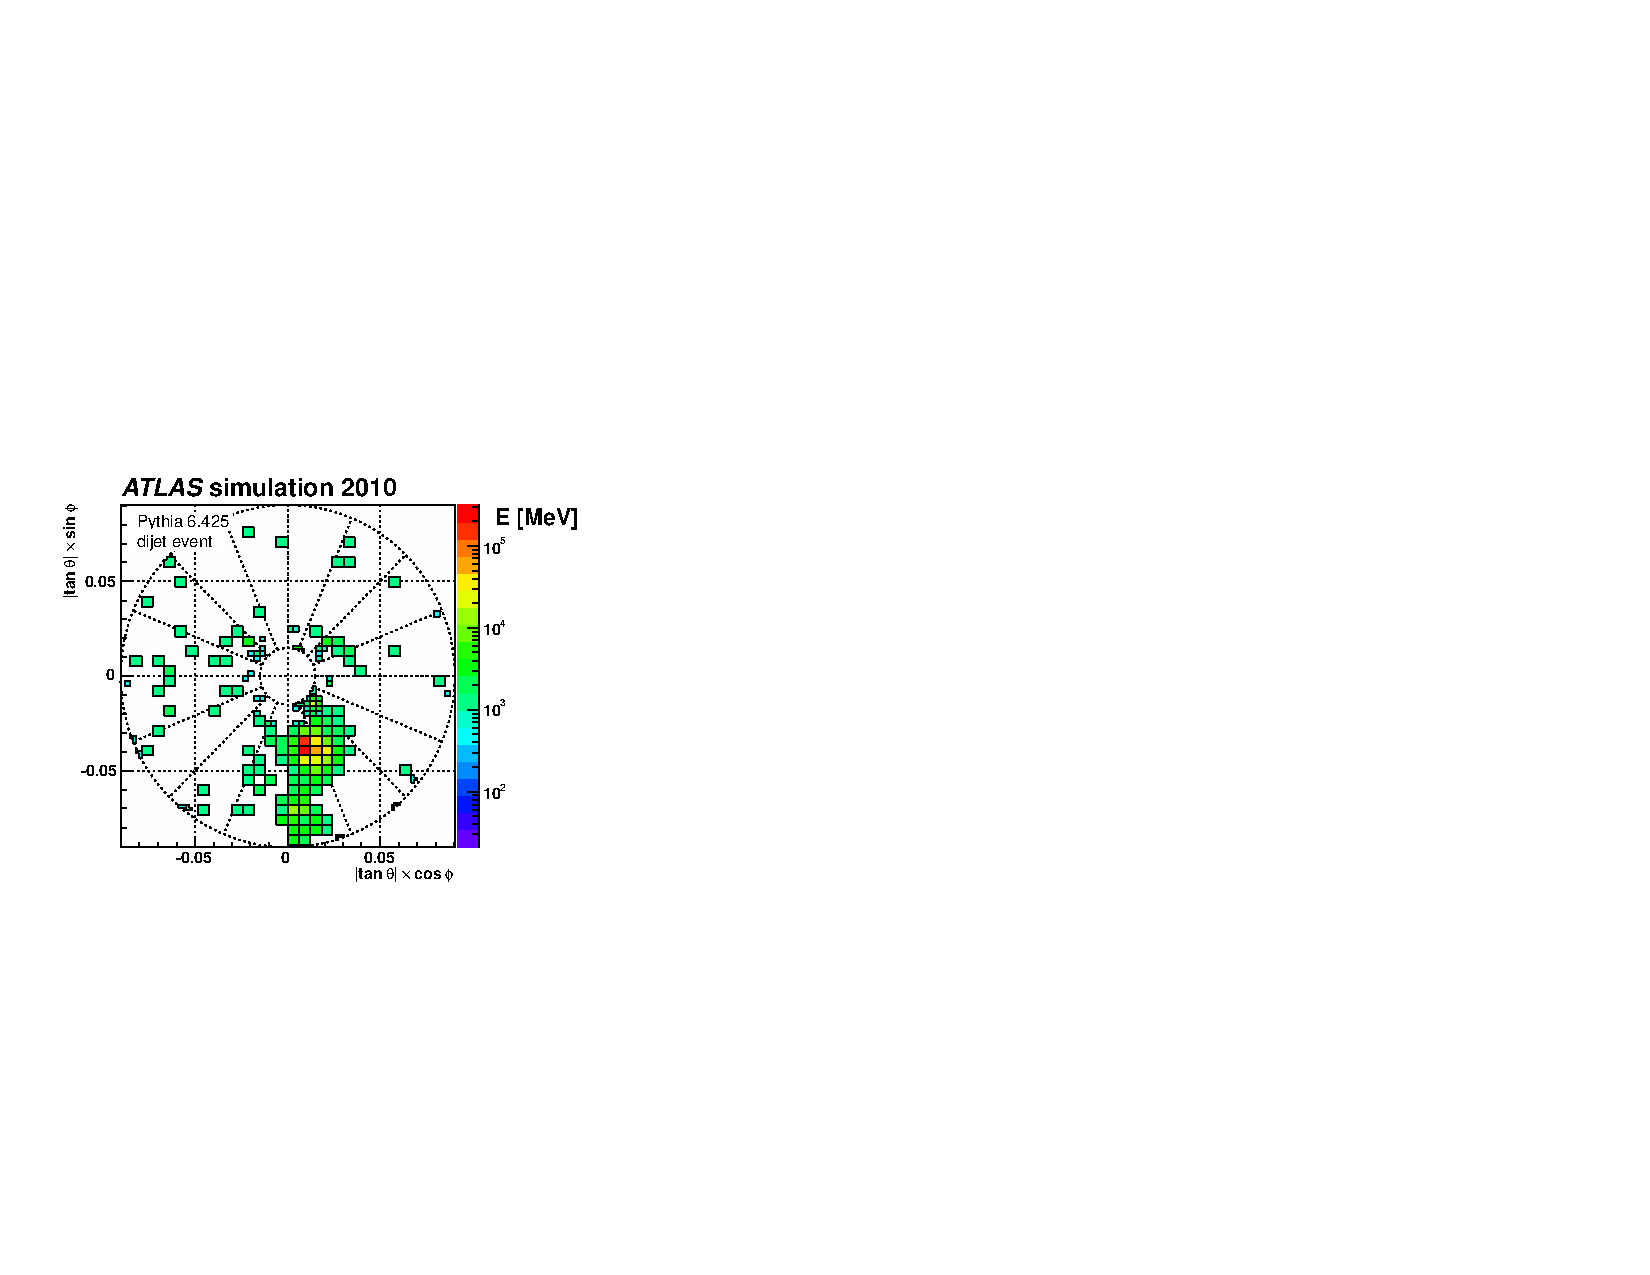
\includegraphics[width=.45\linewidth]{topoclustering_sig2.pdf}} \\
\subfloat[All clustered cells.]{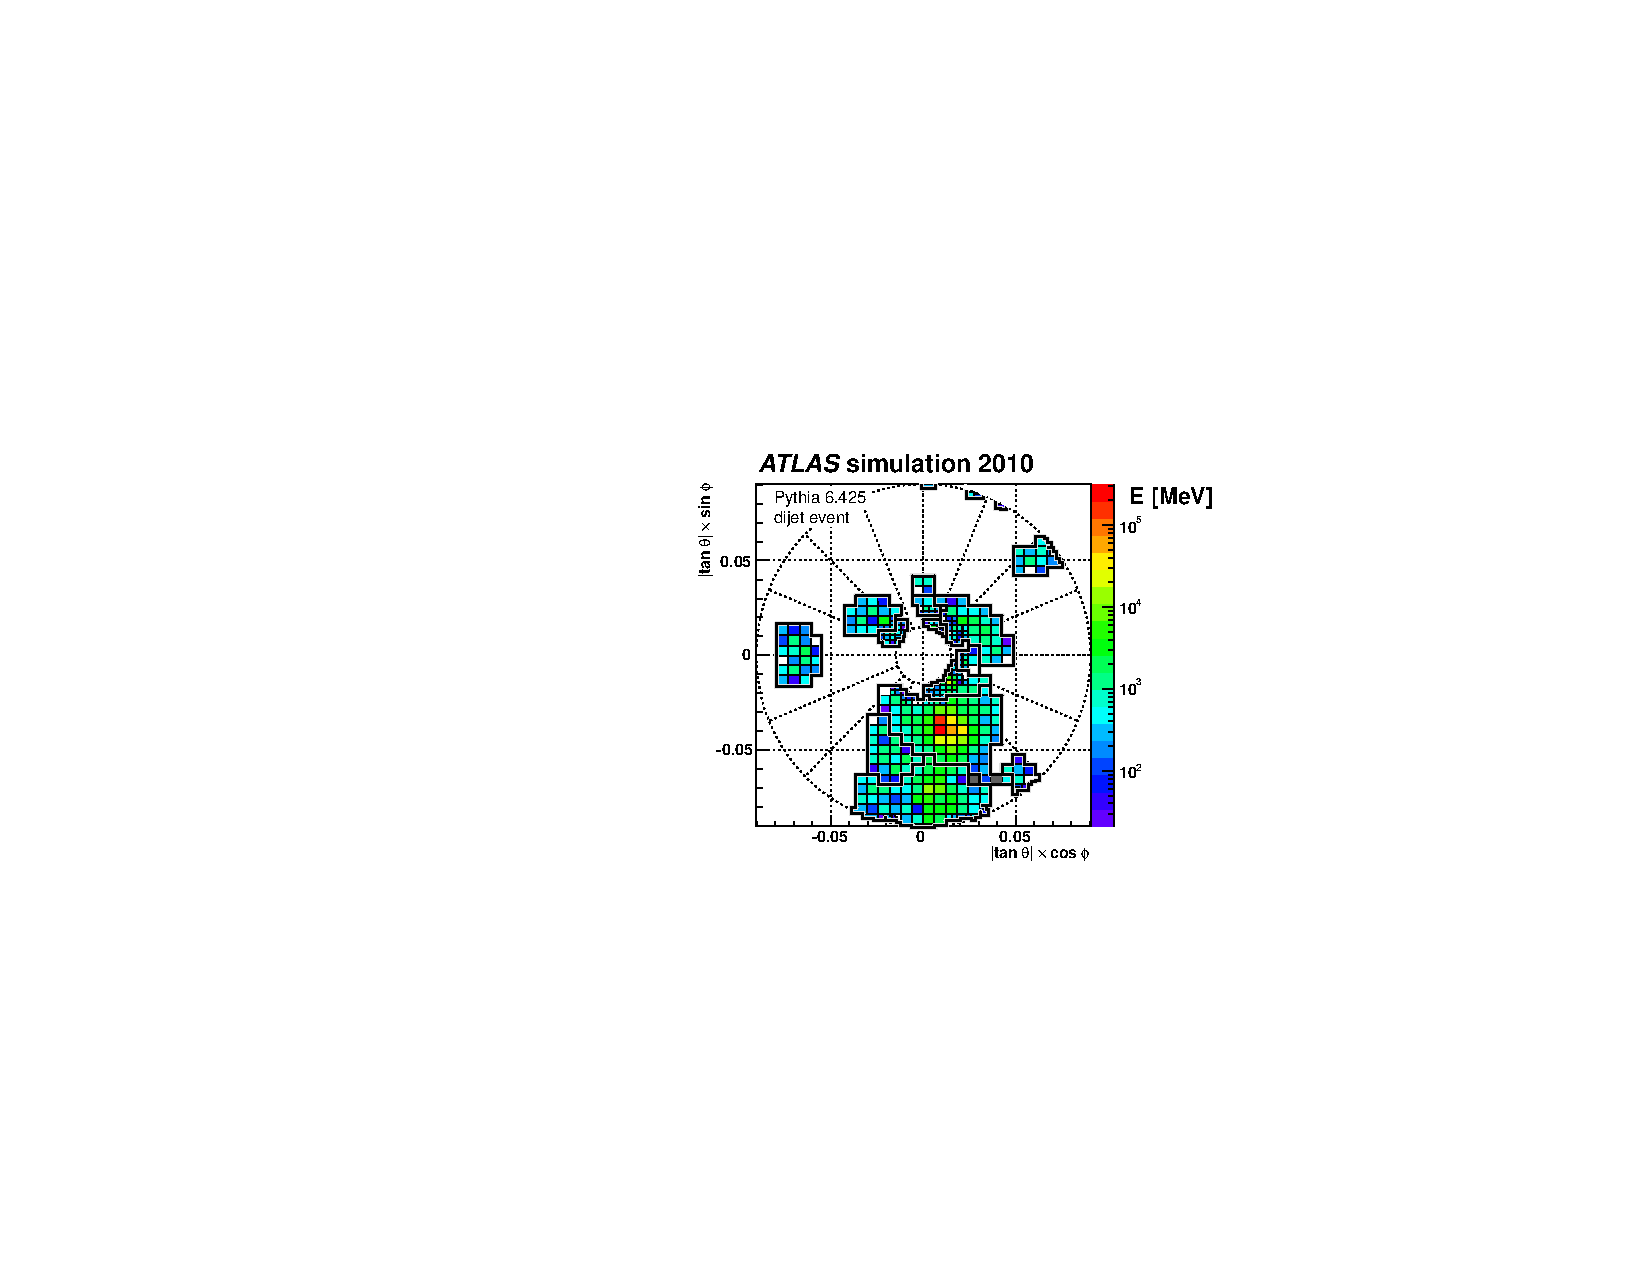
\includegraphics[width=.9\linewidth]{topoclustering_sig0.pdf}}
\end{figure}

There are two calibrations used for clusters.\todo{cite}
These are known as the electromagnetic (EM) scale and the local cluster weighting (LCW) scale.
The EM scale is the energy read directly out of the calorimeters as described.
This scale is appropriate for electromagnetic processes.
The LCW scale applies additional scaling to the clusters based on the shower development.
This allows the cluster energy to be corrected for calorimeter non-compensation and the differences in the hadronic and electromagnetic calorimeters' responses.
This scale provides additional corrections that improve the accuracy of hadronic energy measurements.
This thesis only uses the EM scale corrections unfortunately; LCW scaling requires additional measurements that only became available with additional data.
Due to the jet calibration procedure that we will describe below, it is also a relatively complicated procedure to rederive the ``correct'' jet energy.

\subsection{Muon Spectrometer Tracks}\label{sec:ms_tracks}

Muon spectrometer tracks are fit using the same algorithms as the ID tracks, but different subdetectors.
The tracks are seeded by hits in the MDTs or CSCs.
After seeding in the MDTs and CSCs, the hits from all subsystems are refit as the final MS track.
These tracks are used as inputs to the muon reconstruction, as we will see below.

\section{Physics Object Reconstruction and Quality Identification}

There are essentially six objects used in ATLAS searches for new physics: electrons, photons, muons, $\tau$-jets, jets, and \met.
The reconstruction of these objects is described here; in this thesis, $\tau$ lepton jets are not treated differently from other hadronic jets.
A very convenient summary plot is shown in Fig.\ref{fig:atlas_interactions}.
\begin{figure}
\caption{The interactions of particles with the ATLAS detector.
Solid lines indicate the particle is interacting with the detector, while dashed lines are shown where the particle does not interact.} \label{fig:atlas_interactions}
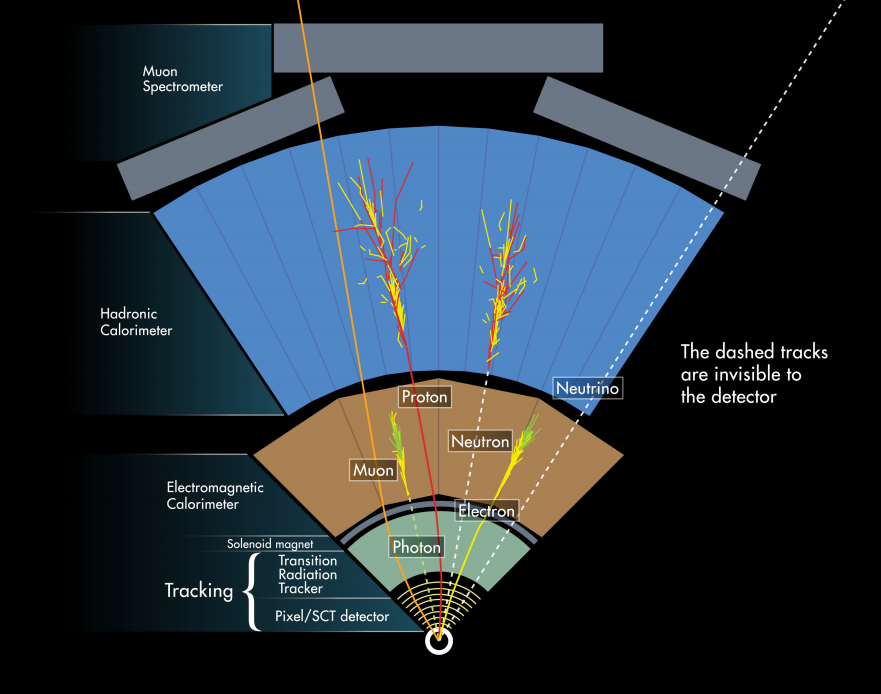
\includegraphics[width=.9\linewidth]{atlas_particle_interactions}
\end{figure}
This process produces candidate objects, which are then identified by quality.

One often wishes to understand ``how certain'' we are that a particular object is truly the underlying physics object.
In ATLAS, we often generically consider, in order, \textit{very loose}, \textit{loose}, \textit{medium}, and \textit{tight} objects\footnotemark.
\footnotetext{
These are not all used for all objects, but it's conceptally useful to think of these different categories.
}
These are ordered in terms of decreasing object efficiency, or equivalently, decreasing numbers of fake objects.
We will also describe briefly the classification of objects into these categories.

In this thesis, we present a search for new physics in a zero lepton final state; we will provide additional details about jet and \met reconstruction.
% \subsection{Vertices}

% Vertex reconstruction is an important first step in the reconstruction of ATLAS events\cite{ATL-INDET-PUB-2009-001}.
% If two tracks from charged particles point at the same place inside the detector, we can associate these tracks to that point, which we then call a vertex.
% Generally, we speak of primary vertices associated
% \begin{figure}
% \caption{Depiction of different vertices reconstruct by ATLAS.
% Each ATLAS event has the primary vertex, b-physics vertices, and pileup vertices.} \label{fig:topocluster}
% 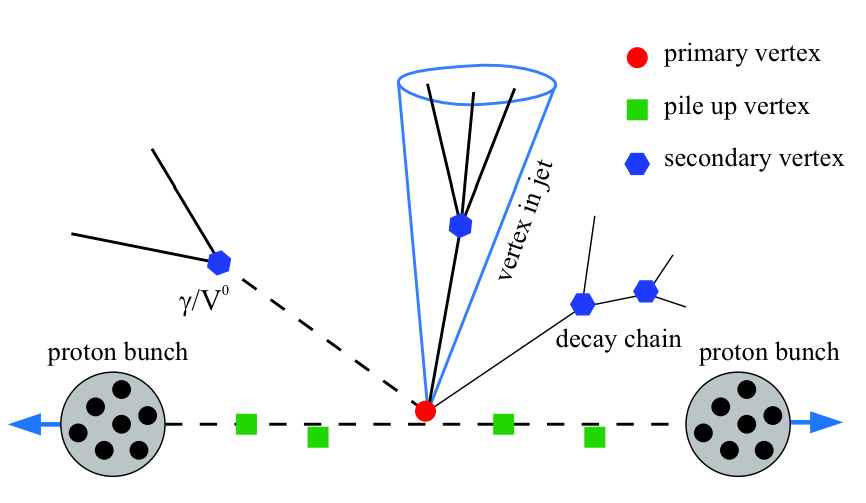
\includegraphics[width=.45\linewdith]{vertex_reconstruction} \\
% \end{figure}

\subsection{Electrons and Photons}

\subsubsection{Reconstruction}
The reconstruction of electrons and photons (often for brevity called ``electromagnetic objects'') is very similar \cite{Aaboud:2016yuq,PERF-2013-05, PERF-2013-03 }.
This is because the reconstruction begins with the energy deposit in the calorimeter in the form of an electromagnetic shower.
For any incoming $e/\gamma$, this induces many more electrons and photons in the shower; the measurement in the calorimeter is similar for these two objects.

One thus begins the reconstruction of electromagnetic objects from the sliding-window clusters reconstructed from the EM calorimeter, as described in Sec.\ref{sec:id_tracks}.
These $E > 2.5 \GeV$ clusters the the primary seed for electrons and photons.
One then looks for all ID tracks within $\Delta R < 0.3$.\todo{check delta R defined somewhere}
We ``match'' the track and cluster if they are within $\Delta \phi < 0.2$ in the direction of track curvature, or $\Delta \phi < 0.05$ in the direction opposite the track curvature.
Those track-cluster seeds with tracks pointing to the primary vertex are reconstructed as electrons.

For photons, we have two options to consider, known as \textit{converted} and \textit{unconverted} photons.
Due to the high energy of the LHC collisions, typical photons have energy $\order 1 \GeV$; at this scale, photons interact almost exclusively via pair-production in the presence of the detector material \todo{DIAGRAM}.
If the track-cluster seed has a track which does not point at the primary vertex, we reconstruct this object as a converted photon.
This happens since the photon travels a distance before decay into two electrons, and see the tracks coming from this secondary vertex.
Those clusters which do not have any associated tracks are then reconstruced as an unconverted photon.

The final step in electromagnetic object reconstruction is the final energy value assigned to these objects; this process is different between electrons and photons due to their differing signatures in the EM calorimeter.
In the barrel, electrons energies are assigned as the sum of the 3 clusters in $\eta$ and 7 clusters in $\phi$ to account for the electron curving in the $\phi$ direction.
Barrel photons are assigned the energy sum of $(3,5)$ clusters in $(\eta, \phi)$ space.
In the endcap, the effect of the magnetic field on the electrons is smaller, and there is a coarser granularity.
Both objects sum the $(5,5)$ clusters for their final energy value.

\subsubsection{Quality Identification}

Electrons have a number of important backgrounds which can give fakes.
Fake electrons come primarily from secondary vertices in hadron decays or misidentified hadronic jets.
To reduce these backgrounds, quality requirements are imposed on electron candidates.
Loose electrons have requirements imposed on the shower shapes in the electromagnetic calorimeter and on the quality of the associated ID track.
There is also a requirement that there is a small energy deposition in the hadronic calorimeter behind the electron, to avoid jets being misidentified as electrons (low hadronic leakage).
Medium and tight electrons have increasingly stronger requirements on these variables, and additional requirements on the isolation (as measured by $\Delta R$) and matching of the ID track momentum and the calorimeter energy deposit.

Photons are relatively straightforward to measure, since there are few background processes\cite{ATL-PHYS-PUB-2016-015}.
The primary one is pion decays to two photons, which can cause a jet to be misidentified as photon.
Loose photons have requirements on the shower shape and hadronic leakage.
Tight photons have tighter shower shape cuts, especially on the high granularity first layer of the EM calorimeter.
The efficiency for unconverted tight photons as a function of $\pt$ is should in
\begin{figure}
\caption{Unconverted photon efficiency as measured in \cite{ATL-PHYS-PUB-2016-015}.} \label{fig:photon_eff}
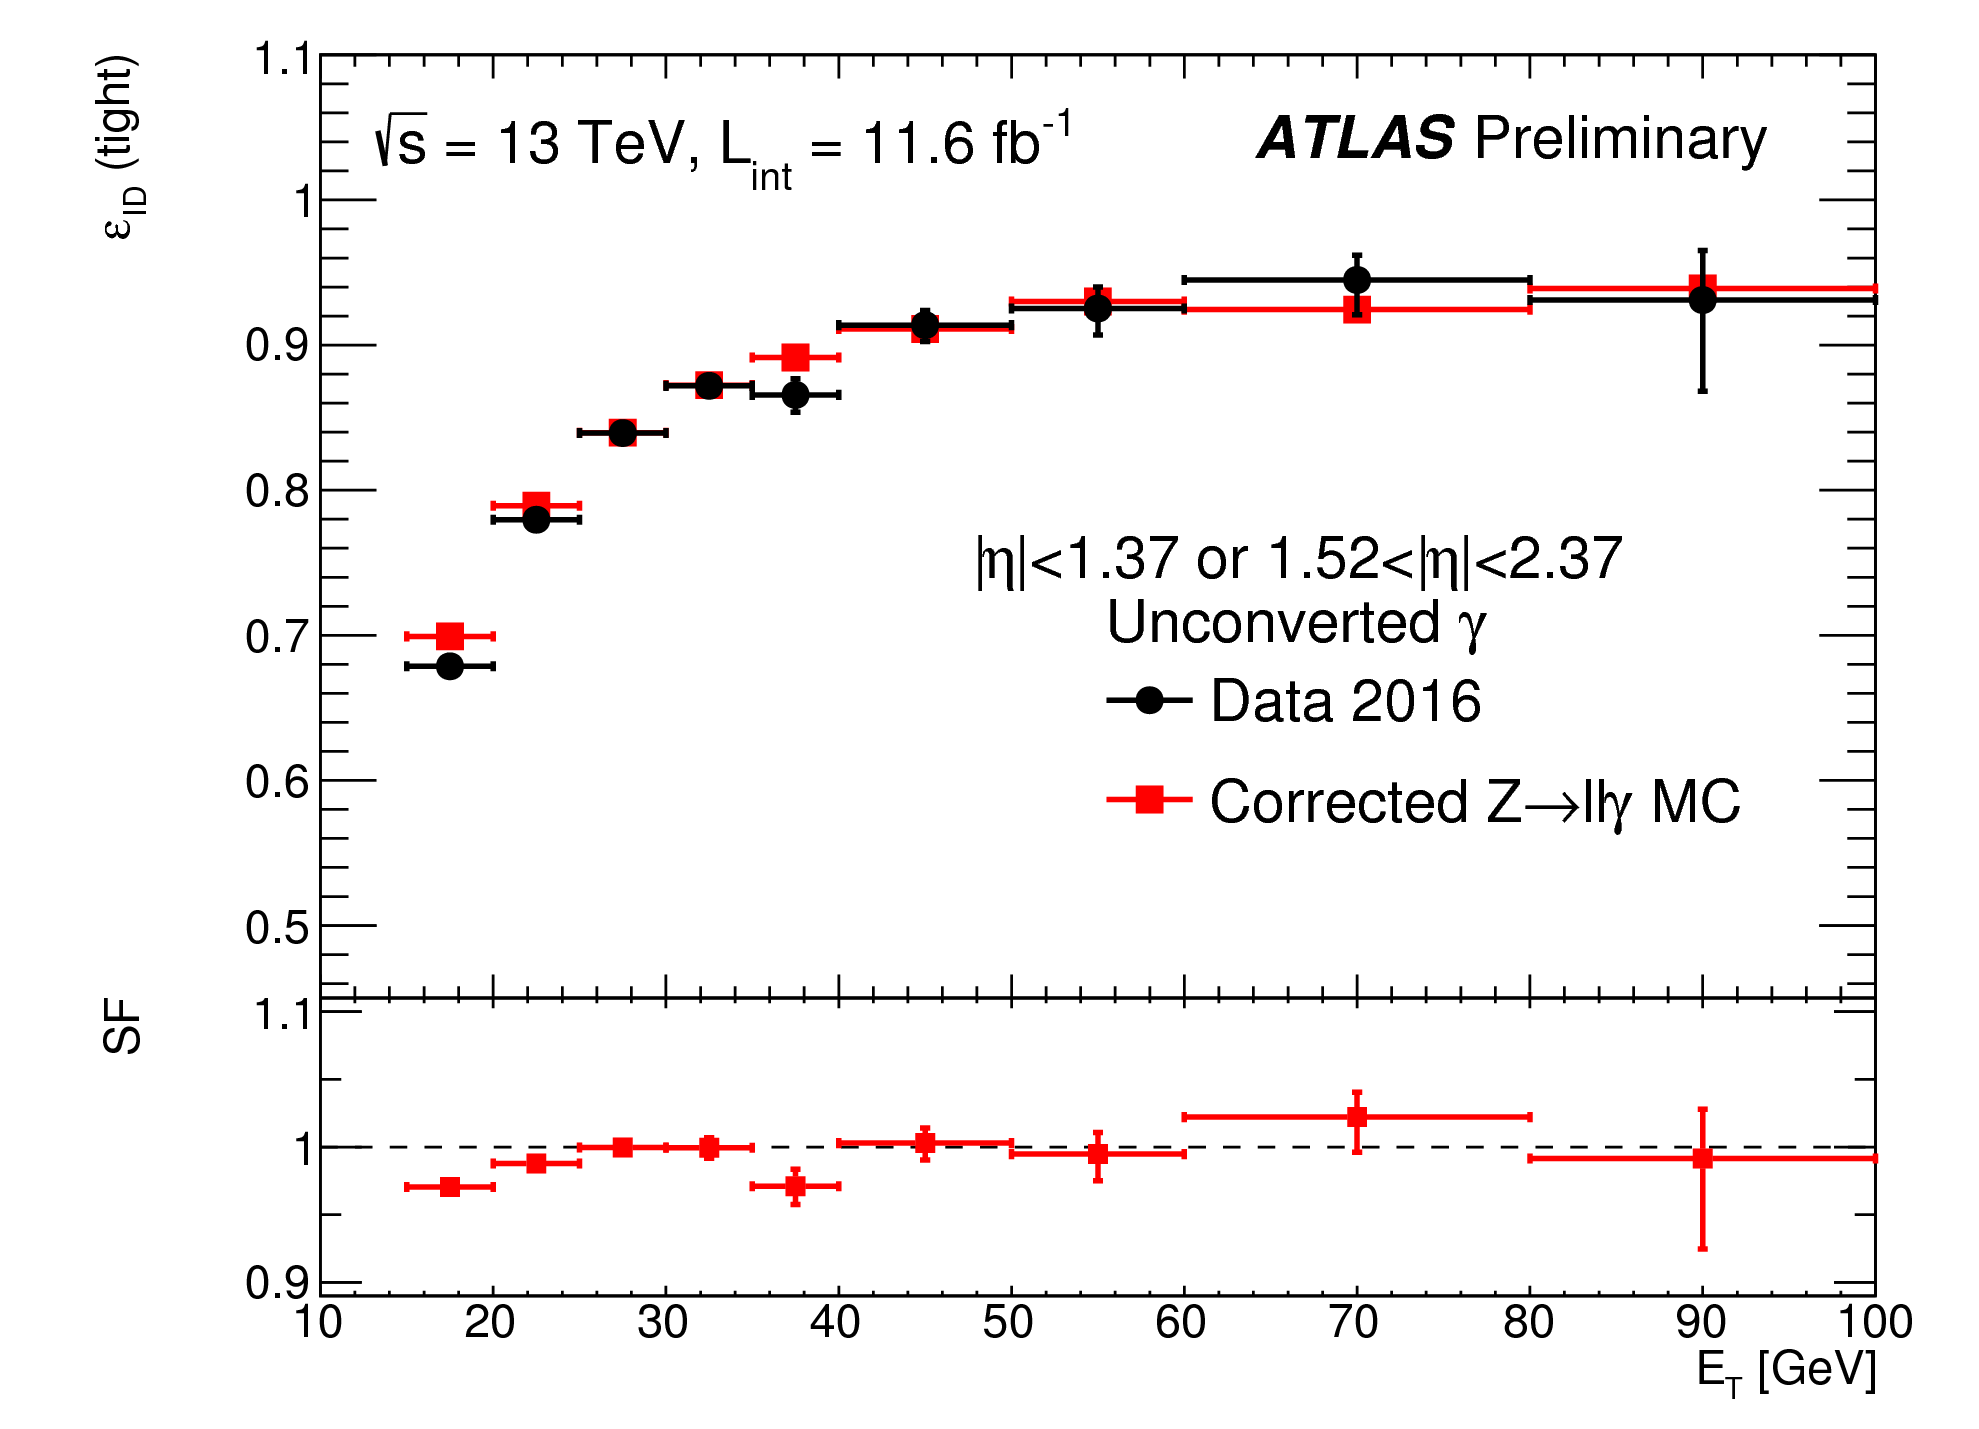
\includegraphics[width=.9\linewidth]{photon_efficiency}
\end{figure}

\subsection{Muons}

\subsubsection{Reconstruction}

Muons are reconstructed using measurements from all levels of the ATLAS detector\cite{PERF-2015-10}.
They leave a ID track, a small, characteristic deposition in the EM calorimeter, and then a track in the muon spectrometer.
The primary reconstruction technique produces a so-called \textit{combined} muon.
``Combined'' means using a combination of the ID and MS tracks to produce the final reconstruced muon kinematics.
This is done by refitting the hits associated to both tracks, and using this refit track for the muon kinematics.
This process produces the best measured muons, although several other worse algorithms are used when the full detector information is missing.
An example is in the region $2.5 < |\eta| < 2.7$ outside the ID acceptance; in this region, MS tracks are used without the corresponding ID tracks.

\subsubsection{Quality Identification}

Several additional criteria are used to assure muon measurements are free of significant background contributions, especially from pion and kaon decays to muons.
Muons produced via these decay processes are often characterized by a ``kink''.
Candidate muons with a poor fit quality, characterized by $\chi^2/\text{n.d.f.}$, are thus rejected.
Additionally, the absolute difference in momentum measurements between the ID and MS provide another handle, since the other decay products from hadron decays carry away some amount of the initial hadron momentum.
This is measured by
\begin{equation}
\rho' = \frac{|\pt^{\text{ID}} - \pt^{\text{MS}} |}{\pt^{\text{Combined}}}.
\end{equation}
Additionally, there is a requirement on the $q/p$ significance, defined as
\begin{equation}\label{eq:muon_sig}
S_{q/p} = \frac{|(q/p)^{\text{ID}} - (q/p)^{\text{MS}} |}{\sqrt{\sigma_{\text{ID}}^2 + \sigma_{\text{MS}}^2  }}.
\end{equation}
The $\sigma_{\text{ID,MS}}$ in the denominator of Eq.\ref{eq:muon_sig} are the uncertainties on the corresponding quantity from the numerator.
Finally, cuts are placed on the number of hits in the various detector elements.

Subsequently tighter cuts on these variables allow one to define the different muon identification criteria.
Loose muons have the highest reconstruction efficiency, but the highest number of fake muons, since there are no requirements on the number of subdetector hits and the loosest requirements on the suite of quality variables.
Medium muons consist of Loose muons with tighter cuts on the quality variables; they also require more than three MDT hits in at least two MDT layers.
These are the default used by ATLAS analyses.
Tight muons have stronger cuts than those of the medium selection, and reducing the reconstruction efficiency.
The reconstruction efficiency as a function of \pt can be seen for Medium muons in Fig.\ref{fig:muon_eff}.

\begin{figure}
\caption{Medium muon efficiency as measured in \cite{PERF-2015-10}.} \label{fig:muon_eff}
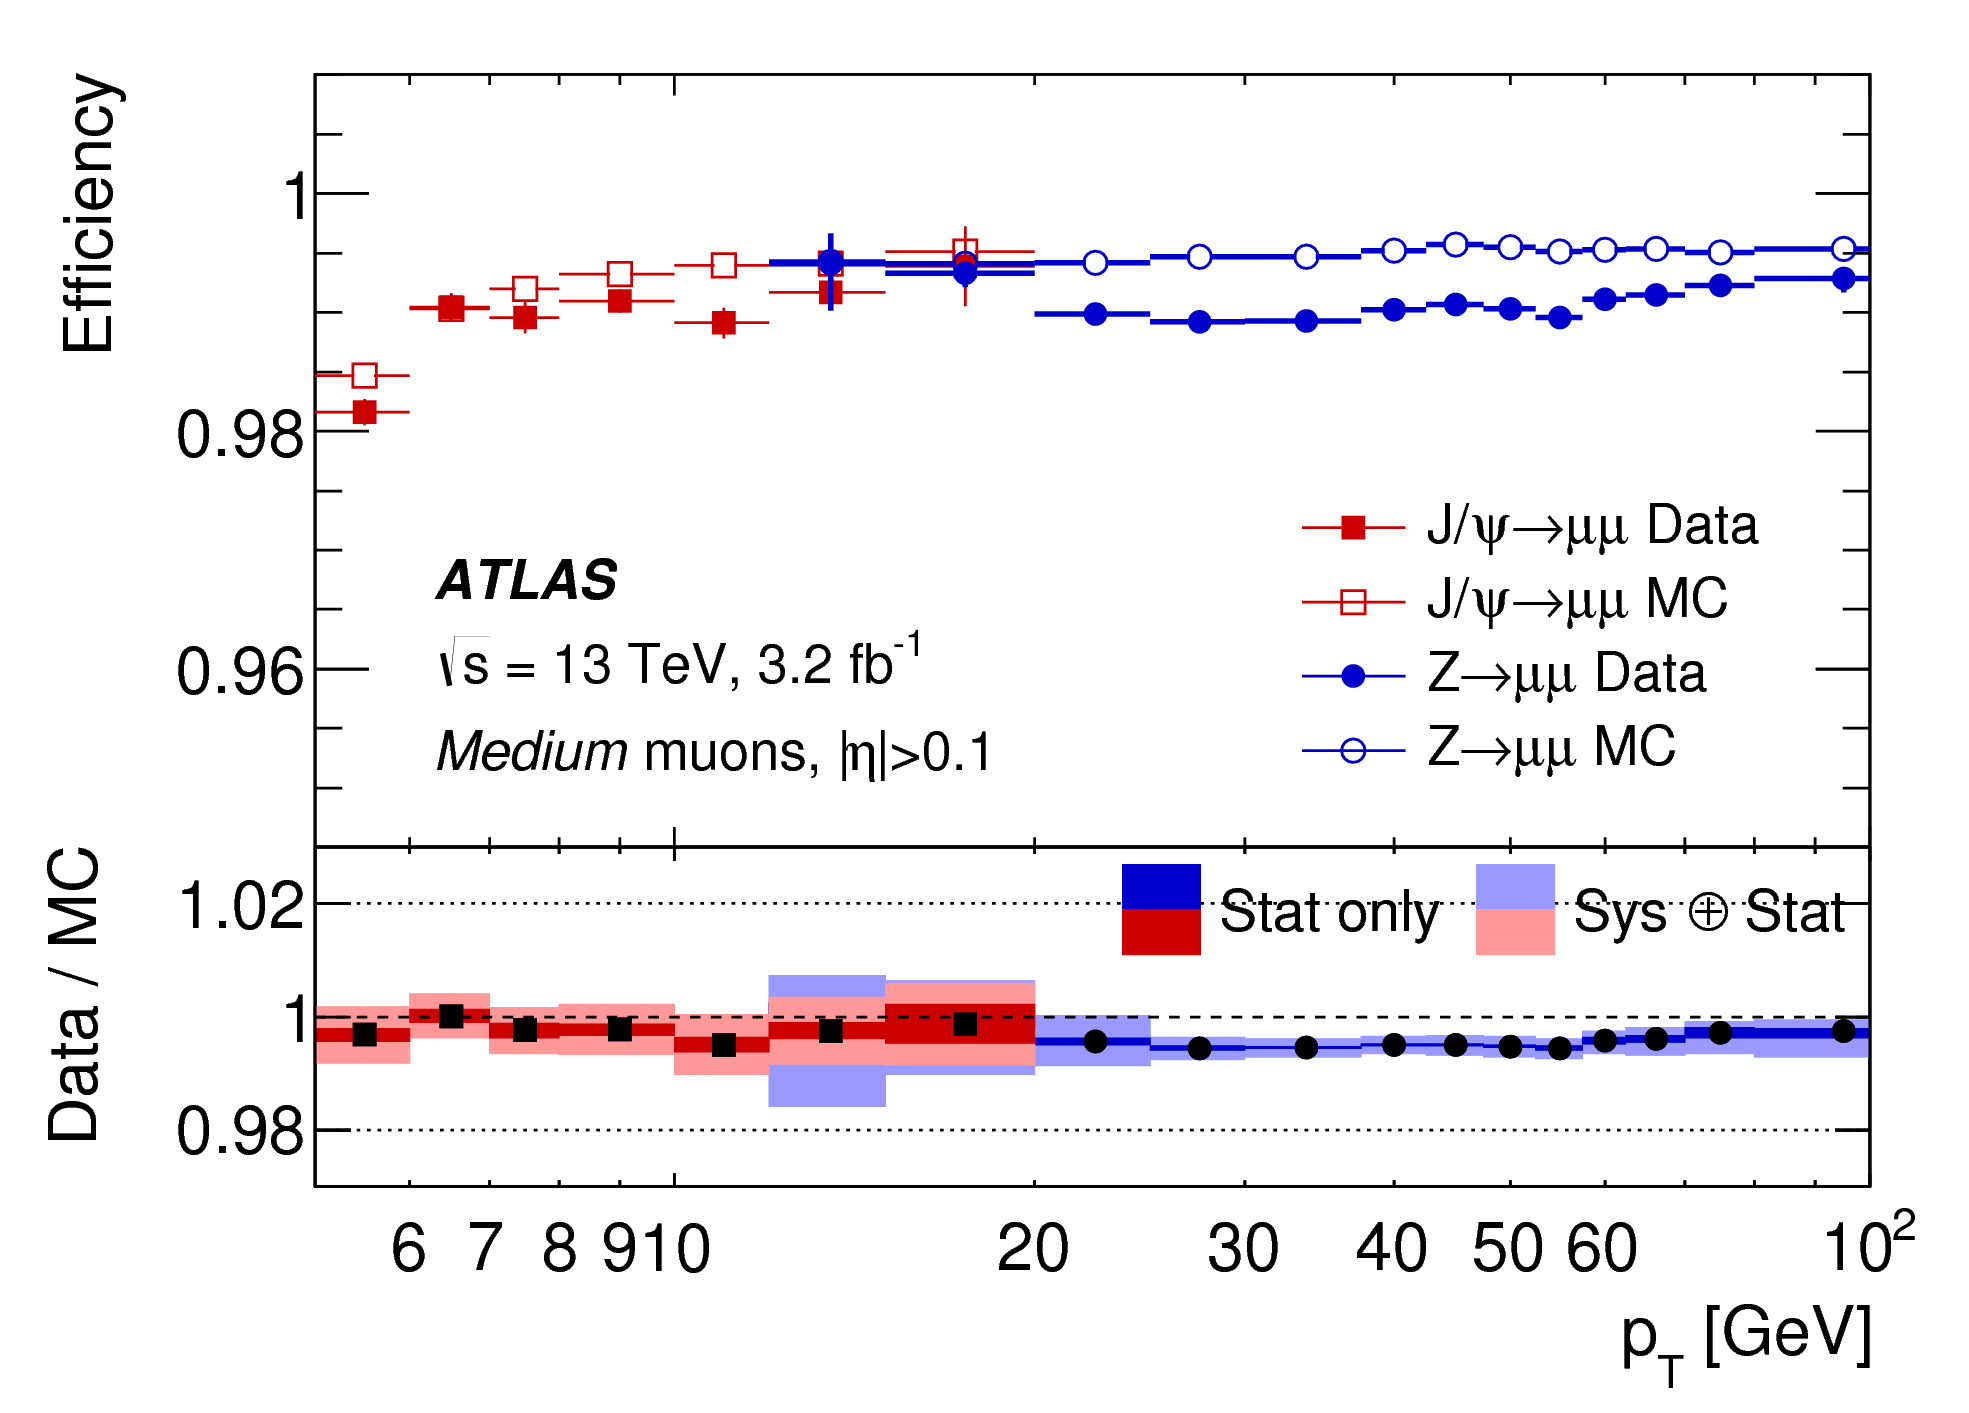
\includegraphics[width=.9\linewidth]{muon_efficiency}
\end{figure}

\subsection{Jets}
\todo{cite paper/note}

Jets are composite objects corresponding to many physical particles.
This is a striking difference from the earlier particles.
Fortunately, we normally (and in this thesis) care about the original particle produced in primary collision.
In the SM, this corresponds to quarks and gluons; due to the hadronization process described in \ref{ch:sm}, free quarks and gluons spontaneously hadronize and produce a hadronic shower, which we call a jet.
These showers can be measured by the EM and hadronic calorimeters, and the charged portions can be measured in the ID.
The first question is how to combine these measurements into a composite object representing the underlying physical parton.
This is done via jet algorithms.

\subsection{Jet Algorithms}

It might seem straightforward to combine the underlying physical particles into a jet.
There are three important characteristics required for any jet reconstruction algorithm to be used by ATLAS.
\begin{itemize}
\item Collinear safety - if any particle with four-vector $p$ is replaced by two particles of $p_1, p_2$ with $p = p_1 + p_2$, the subsequent jet should not change
\item Radiative (infrared) safety - if any particle with four-vector $p$ radiates a particle of energy $\alpha \rightarrow 0$, the subsequent jet should not change
\item Fast - the jet algorithm should be ``fast enough'' to be useable by ATLAS computing resources
\end{itemize}
The first two requirements can be seen in terms of requirements on soft gluon emission.
Since partons emit arbitrarily soft gluons freely, one should expect the algorithms to not be affected by this emission.
The final requirement is of course a practical limitation.

The algorithms in use by ATLAS (and CMS) which satisfies these requirements are collectively known as the \kt algorithms \cite{Ellis:1993tq,Cacciari:2005hq,Cacciari:2008gp}.
These algorithms iteratively combine the ``closest'' objects, defined using the following distance measures :
\begin{equation}
\begin{aligned}\label{eq:kt}
d_{ij} &= \text{min}(k_{T,i}^{2p} , k_{T,j}^{2p} )  \frac{\Delta_{ij}^2 }{R^2} \\
d_{iB} &= k_{T_i}^{2p}
\end{aligned}
\end{equation}
In Eq.\ref{eq:kt}, $k_T,i$ is the transverse momentum of $i$-th jet \textit{constituent}, $\Delta_{ij}$ is the angular distance between the constituents.
Both $R$ and $p$ are adjustable parameters; $R$ is known as the (jet) \textit{cone size} and $p$ regulates the power of the energy vs the geometrical scales.
The algorithm sequence, for a given set of objects $i$ with four-vector $k$ :
\begin{enumerate}
\item Find the minimum distance in the set of all $d_{ij}$ and $d_{iB}$.
\item If the distance is one of the $d_{ij}$, combine the input pair of object $i,j$ and return to (1).
If the distance is one of the $d_{iB}$, remove the object from the list, call it a jet, and return to (1).
\end{enumerate}
This process ends when all objects $i$ have been added to a jet.

Any choice of $(p,R)$ has the requirements of collinear and radiative safety.
In essence, the choice is then to optimize based on speed and the potential for new physics discoveries.
In ATLAS, we make the choice of $p = -1$; this is also known as the \textit{anti-}\kt algorithm.
The choice of $R = 0.4$ is used for the distance parameter of the jets.

The primary ``nice'' quality of this algorithm can be seen with the following example.
Consider three inputs to an anti-\kt algorithm, all with $\eta = 0$ :
\begin{itemize}
\item Object 1 : (\pt, $\phi$) = (30 \GeV, 0)
\item Object 2 : (\pt, $\phi$) = (20 \GeV, -0.2)
\item Object 3 : (\pt, $\phi$) = (10 \GeV, 0.2)
\item Object 4 : (\pt, $\phi$) = (1  \GeV, 0.5)
\end{itemize}.
In the case shown, it seems natural to first combine the ``bigger'' objects 1 and 2.
These then pick up the extra small object 3, and object 4 is not included in the jet.
This is exactly what is done by the anti-\kt algorithm.
The (normal) \kt algorithm with $p = 1$ instead combines the smallest objects, 3 and 4, first.
Object 1 and 2 combine to form their own jet, instead of these jets picking up object 3.
This behavior is not ideal due to the effects of pileup, as we will see in the next section.

\subsection{Jet Reconstruction}

In ATLAS, jets are reconstructed using multiple different objects as inputs, including tracks, ``truth'' objects, calorimeter clusters, and \textit{particle flow objects} (PFOs) \todo{cite pflow paper}.
For physics analyses, ATLAS primarily uses jets reconstructed from calorimeter clusters, but we will describe the others here, as they are often used for derivations of systematic uncertainties or future prospects.

Calorimeter jets are reconstructed using topoclusters using the anti-\kt algorithm with $R = 0.4$.
The jet reconstruction algorithm is run on the collection of all topoclusters reconstructed as in Sec.\ref{sec:topoclusters}.
Both EM and LCW scale clusters are used in the ATLAS reconstruction software and produce two sets of jets for analysis.
As stated above, this thesis presents an analysis using jets reconstructed using EM scale clusters; we refer to these as \textit{EM jets}.

Tracks can be used as inputs to jet reconstruction algorithms.
Jets reconstructed from tracks are known as \textit{track jets}.
Since the ID tracks do not measure neutral objects, these jets measure an incorrect energy.
However, these are still useful for checks and derivations of systematic uncertainties.

\textit{Truth} jets are reconstructed from \textit{truth} particles.
In this case, truth is jargon for simulation; in simulation, the actual simulated particles are available and used as inputs to the jet reconstruction algorithms.
Similarly to track jets, these are not useful in and of themselves.
Instead, truth jets are used for comparisons and derivations of systematic uncertainties.

The last object generally used as inputs to jet reconstruction algorithms are \textit{particle flow objects} (PFOs) \todo{cite atlas paper and theory paper maybe?}
Particle flow objects are reconstructed by associating tracks and clusters through a combination of angular distance measures and detector response measurements to create a composite object which contains information from both the ID and the calorimeters.
For calorimeter clusters which do not have any associated ID track, the cluster is simply the PFO.
The natural association between tracks and clusters provides easy pileup subtraction since tracks are easily associated to the primary vertex.
This technique is generally used in CMS, and ATLAS has been slow to adopt the same.
As pileup has increased, the utility of using PFOs as inputs to jet reconstruction has increased as well.

\subsection{Jet Calibration}

Jets as described in the last section are still \textit{uncalibrated}.
Even correcting the cluster energies using the LCW does not fully correct the jet energy, due to particles losing energy in the calorimeters.
The solution to this is the \textit{jet energy scale} (JES).
The JES is a series of calibrations which on average restore the correct truth jet energy for a given reconstructed jet.
These steps are shown in Fig.\ref{fig:jes_correction_steps} and described here.

The first step is the origin correction; this adjusts the jet to point at the primary vertex.
Next, is the jet-area based pileup correction.
This step subtracts the ``average'' pileup as measured by the energy density $\rho$ outside of the jets and assumes this is a good approximation for the pileup inside the jet.
One then removes energy $\Delta E = \rho \times A_{\text{jet}}$ in this step.
The residual pileup correction makes a final offset correction by parametrizing the change in jet energy as a function of the number of primary vertices $N_{\text{PV}}$ and the average number of interactions $\mu.$

The next step is the most important single correction; it is known as the AbsoluteEtaJES step.
Due to the use of non-compensation and sampling calorimeters in ATLAS, the measured energy of a jet is a fraction of the true energy of the outgoing parton.
Additionally, due to the use of different technologies and calorimeters throughout the detector, there are directional biases induced by these effects.
The correction bins a multiplicative factor in \pt and $\eta$ which scales the reconstructed jets to corresponding truth jet \pt.
This step does not entirely correct the jets, since it is entirely a simulation-based approach.

The final steps are known as the global sequential calibration (GSC) and the residual in-situ calibration.
The GSC uses information about the jet showering shape to apply additional corrections based on the expected shape of gluon or quark jets.
The final step is the residual in-situ calibration, which is only applied to data.
This step uses well-measured objects recoiling off a jet to provide a final correction to the jets in data.
In the low \pt region ($20 \GeV \order< p_{T,\text{jet}}  \order < 200 \GeV $ ), $Z \rightarrow ll$ events are used as a reference object.
In the middle \pt region ($100 \GeV \order< p_{T,\text{jet}}  \order< 600 \GeV $), the reference object is a photon, while in the high \pt region ($p_{T,\text{jet}} \order> 200 \GeV $), the high \pt jet is compared to multiple smaller \pt jets; the reference object is this group of multijets.
After this final correction, the data and MC scales are identical up to the corresponding uncertainties; the combined JES uncertainty as a function of \pt is shown in Fig.\ref{jes_uncertainties}.

\begin{figure}
\caption{The steps used by ATLAS to calibrate jets} \label{fig:jes_correction_steps}
\includegraphics[width=.9\linewidth]{jes_correction_steps}
\end{figure}


\begin{figure}
\caption{Combined jet energy scale uncertainty as a function of \pt at \eta = 0.} \label{fig:jes_uncertainties}
\includegraphics[width=.9\linewidth]{jes_uncertainties}
\end{figure}


\subsection{B-jets}




\subsection{Missing Transverse Momentum}
\todo{cite paper/notes}

\section{Maybe PFlow?}%Reconstruction
%This is the first chapter of the dissertation

%The following command starts your chapter. If you want different titles used in your ToC and at the top of the page throughout the chapter, you can specify those values here. Since Columbia doesn't want extra information in the headers and footers, the "Top of Page Title" value won't actually appear.

\chapter[Table of Contents Title][Top of Page Title]{Title of Chapter 1}

Here you can write some introductory remarks about your chapter.
I like to give each sentence its own line.

When you need a new paragraph, just skip an extra line.

\section*{New Section}

By using the asterisk to start a new section, I keep the section from appearing in the table of contents.
If you want your sections to be numbered and to appear in the table of contents, remove the asterisk.

%LHC
%This is the first chapter of the dissertation

%The following command starts your chapter. If you want different titles used in your ToC and at the top of the page throughout the chapter, you can specify those values here. Since Columbia doesn't want extra information in the headers and footers, the "Top of Page Title" value won't actually appear.

\chapter[Table of Contents Title][Top of Page Title]{Title of Chapter 1}

Here you can write some introductory remarks about your chapter.
I like to give each sentence its own line.

When you need a new paragraph, just skip an extra line.

\section*{New Section}

By using the asterisk to start a new section, I keep the section from appearing in the table of contents.
If you want your sections to be numbered and to appear in the table of contents, remove the asterisk.

%SM   theory
%This is the first chapter of the dissertation

%The following command starts your chapter. If you want different titles used in your ToC and at the top of the page throughout the chapter, you can specify those values here. Since Columbia doesn't want extra information in the headers and footers, the "Top of Page Title" value won't actually appear.

\chapter[Table of Contents Title][Top of Page Title]{Title of Chapter 1}

Here you can write some introductory remarks about your chapter.
I like to give each sentence its own line.

When you need a new paragraph, just skip an extra line.

\section*{New Section}

By using the asterisk to start a new section, I keep the section from appearing in the table of contents.
If you want your sections to be numbered and to appear in the table of contents, remove the asterisk.

%ATLAS detector
%This is the conclusion of the dissertation

\chapter[Conclusion][Conclusion]{Conclusion} %Your conclusion isn't a numbered chapter, so we use the asterisk here.

This thesis presented a search for supersymmetry in hadronic final states.
The dataset was near the highest integrated luminosity sample and used the highest $\sqrt{s}$ proton-proton collisions ever produced in a laboratory.
By the time this thesis is defended, the dataset will expanded further, and

The search detailed in this thesis is the first to use Recursive Jigsaw Reconstruction.
The analysis failed to find an excess, and strong limits were produced on the simplified models of sparticle pair production considered.
It is useful to consider what has been learned by both this analysis, and dozens of other searches for new physics at both ATLAS and CMS.

There are a few stray thoughts we would like to discuss here: $R$-parity conservation and the use of simplified models.
These disparate concepts can be synthesized into a

\todo{do I want to be this strong}
The assumption of $R$-parity is at the heart of a large number of LHC SUSY searches.
$R$-parity can not be too badly broken, as the proton is very stable, as discussed in the Introduction.
However, there is not a particularly good reason to assume that all the $R$-parity violating couplings are zero, as any individual one can be turned on while not inducing the proton decay shown in \Cref{fig:proton_decay}.
The problem is that the imposition of $R$-parity solves two other problems.
As discussed in the Introduction, $R$-parity conservation would lead to a dark matter candidate.
However, we consider this to be a bit of backwards logic which just happens to fit conveniently into another mystery.
Related, and more insidiously, the assumption of $R$-parity makes searches for SUSY much simpler, as \met can be used as a very strong discriminator against QCD backgrounds.
In order to probe the phase space of $R$-parity violating supersymmetry, much more robust ways of modeling QCD backgrounds is a must.

Simplified models provide a useful tool to understand the reach of supersymmetric searches. \todo{cite Martin}
However, they can also lead us astray, as we must make ad-hoc assumptions which are not well-motivated.
The assumption of $R$-parity is one example of this, but others exist.
Although they are not covered directly in this thesis, searches for supersymmetric tops are particularly affected by the branching ratio assumptions.
As both stops and tops have a variety of decay modes, the assumptions can drastically affect the final limits.
In future searches, there must be additional focus on understanding the simplified models inside of the larger space of the MSSM, or even some more complicated supersymmetric theories.

The space of supersymmetric models is \textit{very} large.
Even in the MSSM, we have 120 free parameters, which we have barely begun to explore.
Viewing the landscape from before Run-1, it is easy to see why the strategies detailed here became commonplace.
Essentially, we \textit{expected} to find some sort of new physics, which would help explain the hierarchy problem.
If we even discover one sparticle, with its associated mass and branching ratios, we would drastically reduce the number of free SUSY model parameters.

From our current point of view, this seems na{\"i}ve.
We have yet to find any supersymmetric particle, and much of the MSSM parameter space has been ruled out.
However, we should not yet despair, as there is much more phase space to be explored.
Things will just have to be a little more fun.

\todo{curse of dimensionality}         %Conclusion

%This final section includes your bibliography.

\backmatter

\SingleSpacing %Start single-spacing text before you start the bibliography. We used \bibitemsep earlier in this document to keep bibliography items separated by one line of blank space, but we need to keep the entries themselves single-spaced.
\printbibliography %Print the bibliography. Your bibliography file is defined as Bibliography.bib earlier in this document by the command \addbibresource. It should be kept in the same folder as this file.

\DoubleSpacing %Set roomier body text throughout your writing. The dissertation office requires that you use double-spacing throughout your main body text.
%This is the first chapter of the dissertation

%The following command starts your chapter. If you want different titles used in your ToC and at the top of the page throughout the chapter, you can specify those values here. Since Columbia doesn't want extra information in the headers and footers, the "Top of Page Title" value won't actually appear.

\chapter[The Standard Model][Top of Page Title]{The Standard Model}

Here you can write some introductory remarks about your chapter.
I like to give each sentence its own line.

When you need a new paragraph, just skip an extra line.

\section{Quantum Field Theory}

\todo{cite Yuval's lectures and notes somehow}

In this section, we provide a brief overview of the necessary concepts from Quantum Field Theory (QFT).

In modern physics, the laws of nature are described by the ``action'' $S$, with the imposition of the principle of minimum action. \todo{cite}
The action is the integral over the spacetime coordinates of the ``Lagrangian density'' \Lagr, or Lagrangian for short.
The Lagrangian is a function of ``fields''; general fields will be called $\phi(x^\mu)$, where the indices $\mu$ run over the space-time coordinates.
We can then write the action $S$ as

\begin{equation}
S = \int d^4 x \Lagr[ \phi_i(x^\mu) , \dmu \phi_i(x^\mu)]
\end{equation}

where we have an additional summation over $i$ (of the different fields).
Generally, we impose the following constraints on the Lagrangian :

\begin{enumerate}
\item Translational invariance - The Lagrangian is only a function of the fields $\phi$ and their derivatives $\dmu \phi$
\item Locality - The Lagrangian is only a function of one point $x_\mu$ in spacetime.
\item Reality condition - The Lagrangian is real to conserve probability.
\item Lorentz invariance - The Lagrangian is invariant under the \Poincare group of spacetime.
\item Analyticity - The Lagrangian is an analytical function of the fields; this is to allow the use of pertubation theory.
\item Invariance and Naturalness - The Lagrangian is invariant under some internal symmetry groups; in fact, the Lagrangian will have \textit{all} terms allowed by the imposed symmetry groups. \todo{maybe add in ref here}
\item Renormalizabilty - The Lagrangian will be renormalizable - in practice, this means there will not be terms with more than power 4 in the fields.
\end{enumerate}

The key item from the point of view of this thesis is that of ``Invariance and Natural''.
We impose a set of ``symmetries'' and then our Lagragian is the most general which is allowed by those symmetries.

\section{Symmetries}

Symmetries can be seen as the fundamental guiding concept of modern physics.
Symmetries are described by ``groups''. \todo{cite?}.
To illustrate the importance of symmetries and their mathematical description, groups, we start here with two of the simplest and most useful examples :  \Ztwo and $U(1)$.

\subsection{\Ztwo symmetry}

\Ztwo symmetry is the simplest example of a ``discrete'' symmetry.
Consider the most general Lagrangian of a single real scalar field $\phi(x_\mu)$

\begin{equation} \label{scalarFieldLagrangian}
\Lagr_\phi = \frac{1}{2} \dmu \phi \dmuup \phi - \frac{m^2}{2} \phi^2 - \frac{\mu}{2 \sqrt{2}}  \phi^3 - \lambda \phi^4
\end{equation}

Now we \textit{impose} the symmetry
\begin{equation}
\Lagr(\phi) = \Lagr(- \phi)
\end{equation}

This has the effect of restricting the allowed terms of the Lagrangian.
In particular, we can see the term $\phi^3 \rightarrow - \phi^3$ under the symmetry transformation, and thus must be disallowed by this symmetry.
This means under the imposition of this particular symmetry, our Lagrangian should be rewritten as

\begin{equation}
\Lagr_\phi = \frac{1}{2} \dmu \phi \dmuup \phi - \frac{m^2}{2} \phi^2  - \lambda \phi^4
\end{equation}

The effect of this symmetry is that the total number of  $\phi$ particles can only change by even numbers, since the only interaction term $\lambda \phi^4$ is an even power of the field.
This symmetry is often imposed in supersymmetric theories, as we will see in Chapter 3.

\subsection{$U(1)$ symmetry}

$U(1)$ is the simplest example of a continuous (or \textit{Lie}) group.
Now consider a theory with a single complex scalar field $\phi = \operatorname{Re}\phi + i \operatorname{Im}\phi$

\begin{equation}
\Lagr_\phi = \delta_{i,j} \frac{1}{2} \dmu \phi_i \dmuup \phi_j - \frac{m^2}{2} \phi_i \phi_j - \frac{\mu}{2 \sqrt{2}}  \phi_i \phi_j \phi_k  - \lambda \phi_i \phi_j \phi_k \phi_l
\end{equation}

where $i,j,k,l = Re, Im$.
In this case, we impose the following $U(1)$ symmetry : $\phi \rightarrow e^{i\theta}, \phi^* \rightarrow e^{-i\theta} $.
We see immediately that this again disallows the third-order terms, and we can write a theory of a complex scalar field with $U(1)$ symmetry as

\begin{equation}
\Lagr_\phi =  \dmu \phi \dmuup \phi^* - \frac{m^2}{2} \phi \phi^* -   - \lambda (\phi \phi^*)^2
\end{equation}

\section{Local symmetries}

The two examples considered above are ``global'' symmetries in the sense that the symmetry transformation does not depends on the spacetime coordinate $x_\mu$.
We know look at local symmetries; in this case, for example with a local $U(1)$ symmetry,  the transformation has the form $\phi(x_\mu) \rightarrow e^{i \theta (x_mu)} \phi(x_\mu)$.
These symmetries are also known as ``gauge'' symmetries; all symmetries of the Standard Model are gauge symmetries.

There are wide-ranging consequences to the imposition of local symmetries.
To begin, we note that the derivative terms of the Lagrangian \ref{scalarFieldLagrangian} are \textit{not} invariant under a local symmetry transformation
\begin{equation}
\dmu \phi(x_\mu) \rightarrow \dmu ( e^(i\theta(x_\mu) \phi(x_\mu )) = (1 + i \theta(x_\mu) ) e^(i\theta(x_\mu) \phi(x_\mu )
\end{equation}\todo {GET THIS RIGHT}

This leads us to note that the kinetic terms of the Lagrangian are also not invariant under a gauge symmetry.
This would lead to a model with no dynamics, which is clearly unsatisfactory.

Let us take inspiration from the case of global symmetries.
We need to define a so-called ``covariant'' derivative $\Dmuup$ such that

\begin{equation}
\begin{aligned}
\Dmuup \phi   \rightarrow e^{ i q \theta(x^\mu) \Dmuup \phi} \\
\Dmuup \phi^* \rightarrow e^{-i q \theta(x^\mu) \Dmuup \phi} \\
\end{aligned}
\end{equation}

Since $\phi$ and$\phi^*$ transforms with the opposite phase, this will lead the invariance of the Lagrangian under our local gauge transformation.
This $\Dmuup$ is of the following form

\begin{equation}
\Dmuup = \dmu - i g q A^\mu
\end{equation}

where $A^\mu$ is a vector field we introduce with the transformation law

\begin{equation}
A^\mu \rightarrow A^\mu - \frac{1}{g} \dmu \theta
\end{equation}

and $g $ is the coupling constant associated to vector field.
This vector field $A^\mu$ is also known as a ``gauge'' field.

Since we need to add all allowed terms to the Lagrangian, we define

\begin{equation}
F^{\mu\nu} = A^\mu A^\nu - A^\nu A^\mu
\end{equation}

and then we must also add the kinetic term :

\begin{equation}
\Lagr_{\text{gauge}} = - \frac{1}{4} F^{\mu\nu} F_{\mu\nu}
\end{equation}

The most general renormalizable Lagrangian with fermion and scalar fields can be written in the following form

\begin{equation}
\Lagr = \Lagr_{kin} + \Lagr_{\phi} + \Lagr_\psi +   \Lagr{Yukawa}
\end{equation}

\subsection{Symmetry breaking and the Higgs mechanism}
\label{subsec:symmetry_breaking}
Here we view some examples of symmetry breaking.
We investigate breaking of a global $U(1)$ symmetry and a local $U(1)$ symmetry.
The SM will break the electroweak symmetry $SU(2) x U(1)$, and in Chapter 3 we will see how supersymmetry must also be broken.

There are two ideas of symmetry breaking
\begin{itemize}
\item Explicit symmetry breaking by a small parameter - in this case, we have a small parameter which breaks an ``approximate'' symmetry of our Lagrangian.
An example would be the theory of the single scalar field \ref{scalarFieldLagrangian}, when $\mu << m^2$ and $\mu << \lambda$.
In this case, we can often ignore the small term when considering low-energy processes.
\item Spontaneous symmetry breaking (SSB) - spontaneous symmetry breaking occurs when the Lagrangian is symmetric with respect to a given symmetry transformation, but the ground state of the theory is \textit{not} symmetric with respect to that transformation.
This can have some fascintating consequences, as we will see in the following examples
\end{itemize}
Symmetry breaking a

\subsubsection{U(1) global symmetry breaking}

Consider the theory of a complex scalar field under the $U(1)$ symmetry, or the transformation
\begin{equation}
\phi \rightarrow e^{i\theta} \phi
\end{equation}

The Lagrangian for this theory is
\begin{equation}
\Lagr = \dmuup \phi^{\dag} \dmu \phi + \frac{\mu^2}{2} \phi^{\dag} \phi + \frac{\lambda}{4} (\phi^\dag \phi)^2
\end{equation}

Let us write this theory in terms of two scalar fields, $h$ and $\xi$ : $\phi = (h + i\xi) / \sqrt(2)$.
The Lagrangian can then be written as
\begin{equation}
\Lagr = \dmuup h \dmu h + \dmuup \xi dmu \xi - \frac{\mu^2}{2} (h^2 + \xi^2) - \frac{\lambda}{4}(h^2 + \xi^2)^2
\end{equation}

First, note that the theory is only stable when $\lambda > 0$.
To understand the effect of SSB, we now enforce that $\mu^2 < 0$, and define $v^2 = -\mu^2/\lambda$.
We can then write the scalar potential of this theory as :
\begin{equation}
V(\phi) = \lambda (\phi^\dag \phi - v^2/2)^2
\end{equation}

Minimizing this equation with respect to $\phi$, we can see that the ``vacuum expectation value'' of the theory is
\begin{equation}
2<\phi^\dag \phi> = <h^2 + \xi^2 > = v^2
\end{equation}

We now reach the ``breaking'' point of this procedure.
In the $(h, \xi)$ plane, the minima form a circle of radius $v$.
We are free to choose any of these minima to expand our Lagrangian around; the physics is not affected by this choice.
For convenience, choose $<h> = v, <\xi^2> = 0$.

Now, let us define $h' = h - v , \xi' = \xi $ with VEVs $<h'> = 0 , <\xi'> = 0$.
We can then write our spontaneously broken Lagrangian in the form
\begin{equation}
\Lagr = \frac{1}{2} \dmu h' \dmuup h' +  \frac{1}{2} \dmu \xi' \dmuup \xi' - \lambda v^2 h'^2 - \lambda v h' (h'^2 + \xi'^2 ) - \lambda (h'^2 + \xi'^2)^2
\end{equation}


\todo{CITE THIS PICTURE}
\begin{figure} \label{fig:sombrero}
\caption{Sombrero potential}
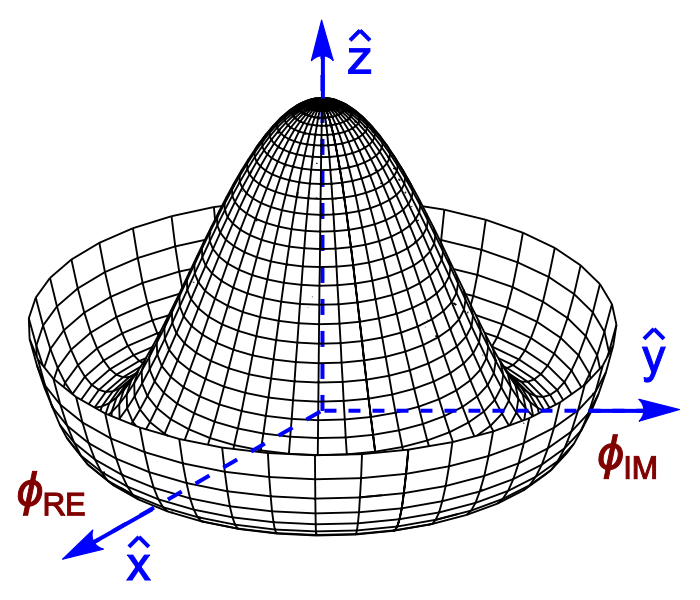
\includegraphics[width=\linewidth]{sombrero_potential}
\end{figure}

\subsubsection{U(1) local  symmetry breaking}

\section{The Standard Model}

\subsection{Overview}

The Standard Model is another name for the theory of the internal symmetry group $SU(3)_C \otimes SU(2)_L \otimes U(1)_Y$ \todo{CHECK}.
This quantum field theory is the culmination of years of work in both theoretical and particle physics.  \todo{cite}

\todo{CITE THIS PICTURE}
\begin{figure}
\caption{The interactions of the Standard Model}
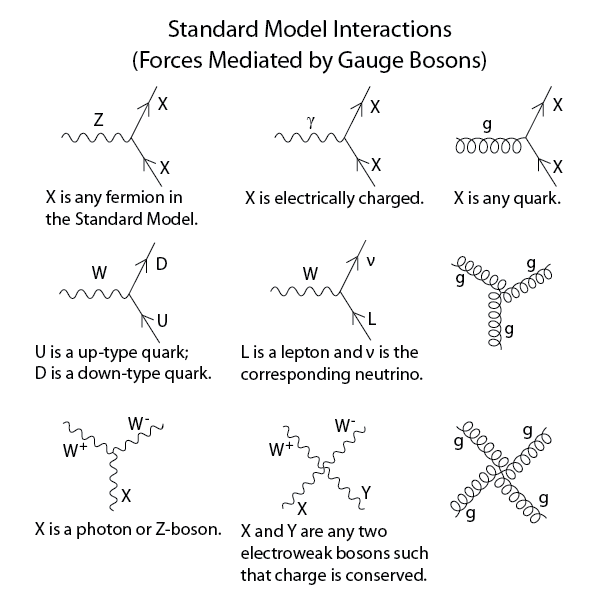
\includegraphics[width=\linewidth]{Standard_Model_Feynman_Diagram_Vertices}
\end{figure}

\subsection{Field Content}

The SM field content is
\begin{equation}
\begin{aligned}
\text{Fermions } Q_L(3,2)_{+1/3}, \xspace  U_R(3,1)_{+4/3},\xspace  D_R(3,1)_{-2/3} ,\xspace  L_L(1,2)_{-1} ,\xspace  E_R(1,1)_{-2}\\
\text{Scalar (Higgs) } \xspace \phi(1,2)_{+1} \\
\text{Vector Fields } \xspace G^\mu(8,1)_0 \xspace W^\mu(1,3)_0  \xspace B^\mu(1,1)_0
\end{aligned}
\end{equation}
where the $(A, B)_Y$ notation represents the irreducible representation under $SU(3)$ and $SU(2)$, with $Y$ being the electroweak hypercharge.
Each of these fields has an additional index, representing the three generation of fermions.

We observed that $Q_L, U_R,$ and $D_R$ are triplets under $SU(3)_C$; these are the \textit{quark} fields.
The ``color'' group, $SU(3)_C$ is mediated by the ``gluon'' field $G^\mu(8,1)_0$, which has 8 degrees of freedom; we say there are 8 gluons.
The fermion fields $L_L(1,2)_{-1}$ and $  E_R(1,1)_{-2} $ are singlets under $SU(3)_C$; we call them \textit{leptons}.

Next, we note the ``left-handed'' (``right-handed'') fermion fields, denoted by $L$ ($R$) subscript,
The left-handed fields form doublets under $SU(2)_L$.
These are mediated by the three degrees of freedom of the  ``W'' fields $W^\mu(1,3)_0$.
These fields only act on the left-handed particles of the Standard Model.
This is the reflection of the ``chirality'' of the Standard Model; the left-handed and right-handed particles are treated differently by the electroweak forces.
The right-handed fields, $U_R, D_R$, and $E_R$, are singlets under $SU(2)_L$.

The $U(1)_Y$ symmetry is associated to the $B^\mu(1,1)_0$ boson with one degree of freedom.
The charge $Y$ is known as the electroweak hypercharge.

\subsection{$\Lagr_{kin}$}

For each of the vector boson fields, we have the follow field strengths :

\begin{equation}
\begin{aligned}
G^{\mu\nu}_a = \dmuup G^\nu_a + \partial^\nu G^\mu_a - g_s f_{abc} G^\mu_b G^\nu_c \\
W^{\mu\nu}_a = \dmuup W^\nu_a + \partial^\nu W^\mu_a - g \epsilon_{abc} W_b^\mu W_c^\nu \\
B^{\mu\nu}   = \dmuup B^\nu   + \partial^\nu B^\mu
\end{aligned}
\end{equation}

where $g$ and $g_s$ are the electroweak and strong coupling constant.

We can write the covariant derivative for the Standard Model as
\begin{equation}
\Dmuup = \dmuup + ig_s G^\mu_a L_a + i g W^\mu_a T_a + i g' Y B^\mu
\end{equation}
where $L_a$ and $T_a$ are the generators of $SU(3)_C $ and $SU(2)_L$ respectively for each of the representations.
Explicitly, for the $SU(3)_C$ triplets, $L_a = \frac{1}{2} \lambda_a$ and for the $SU(3)_C$ singlets, $L_a = 0$. \todo{GELLMANN and Pauli matrices}.
For $SU(2)_L$ doublets, $T_a = \frac{1}{2} \sigma_a $ and for $SU(2)_L$ singlets, $T_a = 0$.

The combination of these terms allows us to write the kinetic terms of the Lagrangian as
\begin{equation}
\begin{aligned}
\Lagr_{kin} = G^{\mu\nu} G_{\mu\nu} + W^{\mu\nu} W_{\mu\nu} + B^{\mu\nu} B_{\mu\nu}\\
 + \Dmuup Q_L \Dmu Q_L + \Dmuup U_R \Dmu U_R +  \Dmuup D_R \Dmu D_R + \Dmuup L_L \Dmu L_LL + \Dmuup E_R \Dmu E_R
\end{aligned}
\end{equation}

\subsection{$\Lagr_{\psi}$ }

We cannot write down any mass terms for fermions in the Standard Model.
Dirac mass terms are forbidden since they are all assigned to ``chiral'' representations of the gauge symmetry.
Majorana mass terms are disallowed since there are no fields with $Y \slashed{=} 0$.

\subsection{$\Lagr_{Yuk}$ }

We write the Yukawa portion of the Standard Model Lagrangian

\begin{equation}
\Lagr_{Yuk} = Y_{ij}\bar{L_{Li} E_{Rj}} \phi + h.c.
\end{equation}

The Yukawa matrix $Y$ is a general complex 3 $\times$ 3 matrix of dimensionless couplings which can be diagonalized, leading to a diagonal matrix with only three real parameters $(y_e , y_\mu , y_\tau)$.
This reflects the fact that for the electron, muon, and tau lepton, the interaction basis is the same as the mass basis; this is the same as saying an electron has a well-defined mass.

\section{$\Lagr_\phi$, Electroweak Symmetry breaking and the Higgs Boson}

Let us now recall that local gauge invariance means that the vector fields in this theory are \textit{massless}.
N\"aively, it seems this combined with the chirality of the Standard Model, that \textit{none} of the fields have masses.
The solution to this seeming conundrum is of course the well-known ``Higgs'' mechanism, described in Sec. \ref{subsec:symmetry_breaking}.

In the Standard Model, the Higgs potential is given by
\begin{equation} \label{eq:higgs_potential}
\Lagr_\phi = -\mu^2 \phi^\dagger \phi - \lambda (\phi^\dagger \phi)^2.
\end{equation}

Since $\lambda$ is dimensionless and real, to have a potential bounded from below, we require $\lambda > 0$.
To break the gauge symmetry, we require $\mu^2 < 0$, leading again to the sombrero potential \ref{fig:sombrero}.
We define
\begin{equation}
v^2 = - \frac{\mu^2}{\lambda}.
\end{equation}

This allows us to write \ref{eq:higgs_potential} as
\begin{equation} \label{eq:higgs_potential_rewritten}
\Lagr_\phi = - \lambda (\phi^\dagger \phi - \frac{v^2}{2})^2
\end{equation}
after dropping the constant term.

This means the $\phi$ field acquires a VEV $|<\phi>| = v/\sqrt{2}$.
Choosing the convenient gauge
\begin{equation}
\phi = \begin{pmatrix} 0 \\ v/\sqrt{2} \end{pmatrix},
\end{equation}

The VEV breaks the $SU(2)_L \otimes U(1)_Y$ symmetry to a $U(1)_{EM}$ subgroup.
We can identify the unbroken generator of this $U(1)_{EM}$ subgroup as $Q_{EM} = T_3 + Y/2$, since this vanishes in the down component
\begin{equation}
Q_{\gamma} \phi = (T_3 + Y/2) \phi = (\frac{1}{2} \sigmathree + \frac{1}{2} I ) \begin{pmatrix} 0 \\ v/\sqrt{2} \end{pmatrix}.
\end{equation}
Here we see the indicative $\gamma$ for the photon, as this unbroken $U(1)_{EM}$ symmetry is of course the symmetry associated to the electromagnetic force mediated by the gauge boson known as the photon.

There are three broken generators : $T_1, T_2, T_3 - Y/2$.
These are each associated to one of the massive gauge bosons induced by the symmetry breaking.
Choosing a gauge which rotates away the ``eaten'' Goldstone boson degrees of freedom, we can write the Higgs field as
\begin{equation}
\label{eq:higgs_field}
\phi = \frac{1}{\sqrt{2}}\begin{pmatrix} 0 \\ v + h(x) \end{pmatrix}.
\end{equation}

\section{Particle Spectrum : Standard Model Lagrangian after Electroweak Symmetry Breaking}

We can now return to the Standard Model Lagrangian and use the equation for the Higgs field after EWSB \ref{eq:higgs_field}.
This will show us the ``physical'' particle content of the Standard Model.

\subsection{Particle content associated to $\Lagr_\phi$}

Setting $phi$ as in Eq.\ref{eq:higgs_field}, we quickly see that we can rewrite Eq.\ref{eq:higgs_potential_rewritten} as
\todo{ CHECK FACTORS OF TWO}
\begin{equation}
\Lagr_\phi = - \lambda (\phi^\dagger \phi - \frac{v^2}{2})^2  = - \lambda ( \frac{1}{2} (v + h(x))^2 - \frac{v^2}{2})^2 = - \lambda ( h(x)^2 + vh(x))^2 = -\lambda ( h(x)^4 + v h(x)^3 + \frac{v^2}{2} h(x)^2 ).
\end{equation}

Interpreting the Higgs field squared term as the mass term of the Higgs boson, we see that $m_H = \sqrt{2 \lambda} v$.

\subsection{Particle content associated to $\Lagr_{kin}$}

Again using Eq.\ref{eq:higgs_field} and $\Dmuup = \dmuup + ig_s G^\mu_a L_a + i g W^\mu_a T_a + i g' Y B^\mu $, we can see how the mass terms associated to the three massive gauge bosons, and also see how the photon stays massless.
The mass terms for the gauge boson fields come from the kinetic term of the Higgs field :
\begin{equation}
\begin{aligned}
\Lagr_{M_V} = \Dmuup \phi \Dmu \phi = (i g W^\mu_a T_a + i g' Y B^\mu ) \frac{1}{\sqrt{2}}\begin{pmatrix} 0 \\ v \end{pmatrix} (i g W_{\mu,a} T_a + i g' Y B_\mu ) \frac{1}{\sqrt{2}}\begin{pmatrix} 0 \\ v \end{pmatrix} = \\
\frac{1}{8} |\begin{pmatrix} gW_3 + g'B & g(W_1 - iW_2) \\ g(W_1 + iW_2) & -gW_3 + g'B \end{pmatrix}  \begin{pmatrix} 0 \\ v \end{pmatrix} |^2
\end{aligned}
\end{equation}
where we have noted that $\dmu$ and $L_a$ both disappear when acting on $\phi$.
Defining the \textit{Weinberg} angle $\tan(\theta_W) = g'/g$ and the following physical fields :
\begin{equation}
\begin{aligned}
W^{\pm} = \frac{1}{\sqrt{2}}(W_1 \mp iW_2) \\
Z^0 = \cos \theta_W W_3 - \sin\theta_W B \\
A^0 = \sin \theta_W W_3 + \cos\theta_W B
\end{aligned}
\end{equation}
we see that we can write the piece of the Lagrangian associated to the vector boson masses as
\begin{equation}
\Lagr_{M_V} = \frac{1}{4} g^2 v^2 W^+ W^- + \frac{1}{8} (g^2 + g'^2)v^2 Z^0 Z^0 .
\end{equation}
and we have the following values of the masses for the vector bosons :
\begin{equation}
\begin{aligned}
m_W^2 = \frac{1}{4} g^2 v^2 \\
m_Z^2 = \frac{1}{4} (g^2 + g'^2) v^2 \\
m_A^2 = 0
\end{aligned}
\end{equation}

\section{Deficiencies of the Standard Model}

By using the asterisk to start a new section, I keep the section from appearing in the table of contents.
If you want your sections to be numbered and to appear in the table of contents, remove the asterisk.

%This is the first chapter of the dissertation

%The following command starts your chapter. If you want different titles used in your ToC and at the top of the page throughout the chapter, you can specify those values here. Since Columbia doesn't want extra information in the headers and footers, the "Top of Page Title" value won't actually appear.

\chapter[Additional N-1 plots][Top of Page Title]{The Standard Model}
\label{app:n-1_plots}

\todo{add some text or cut this}

\section{Compressed region N-1 plots}

\begin{figure}[tbph]
\begin{center}
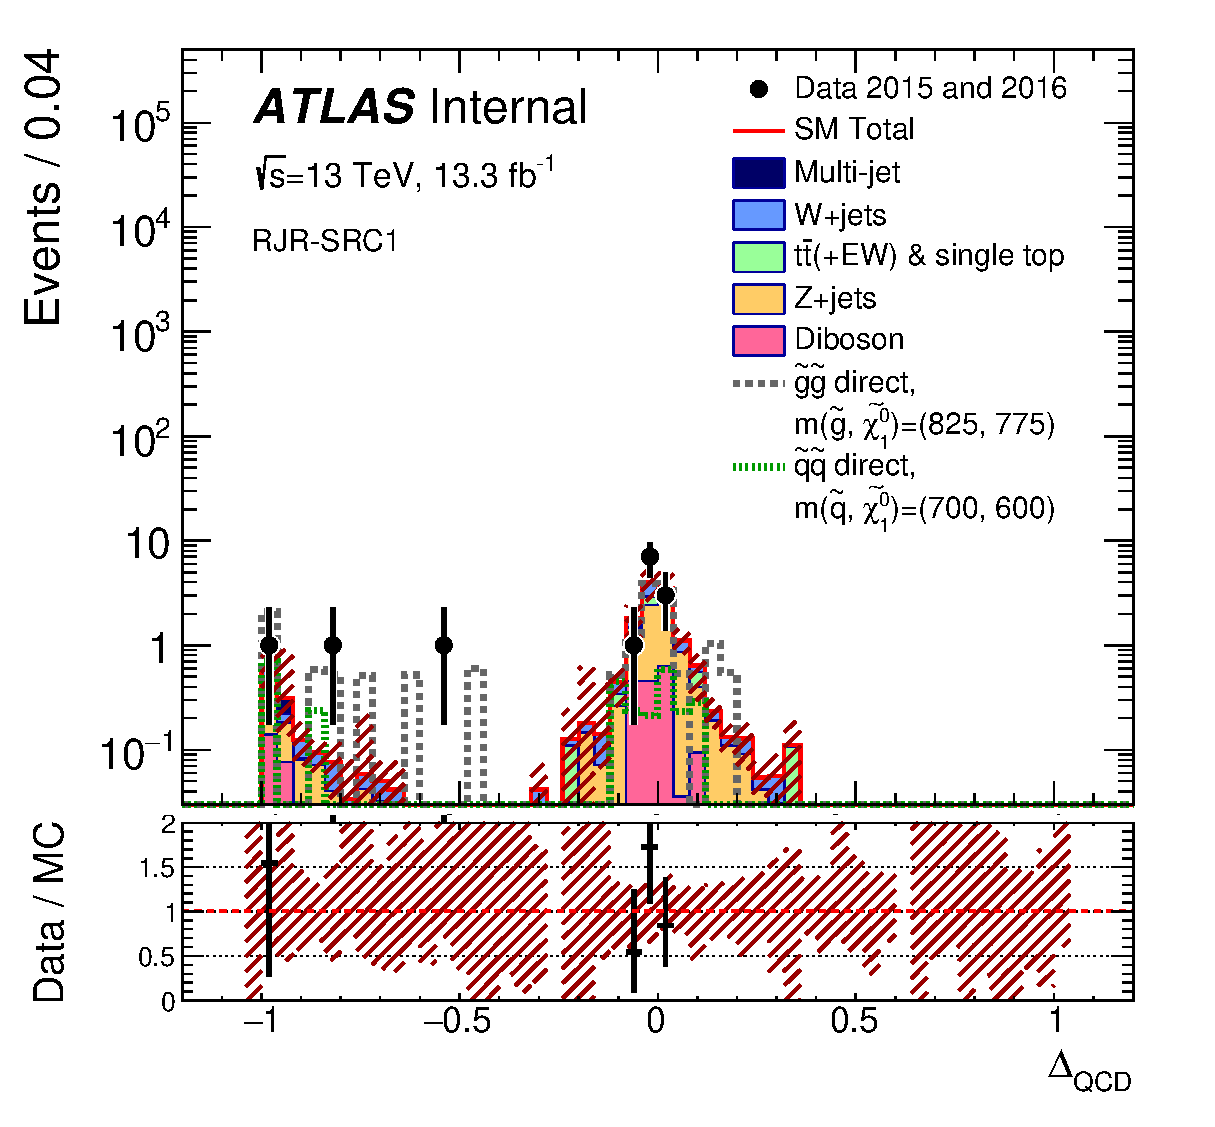
\includegraphics[width=0.33\textwidth]{ATLAS-CONF-2016-078_INT/N-1Plots/AtlasStyle/SR_SRJigsawSRC1_deltaQCD_SR_minusone}
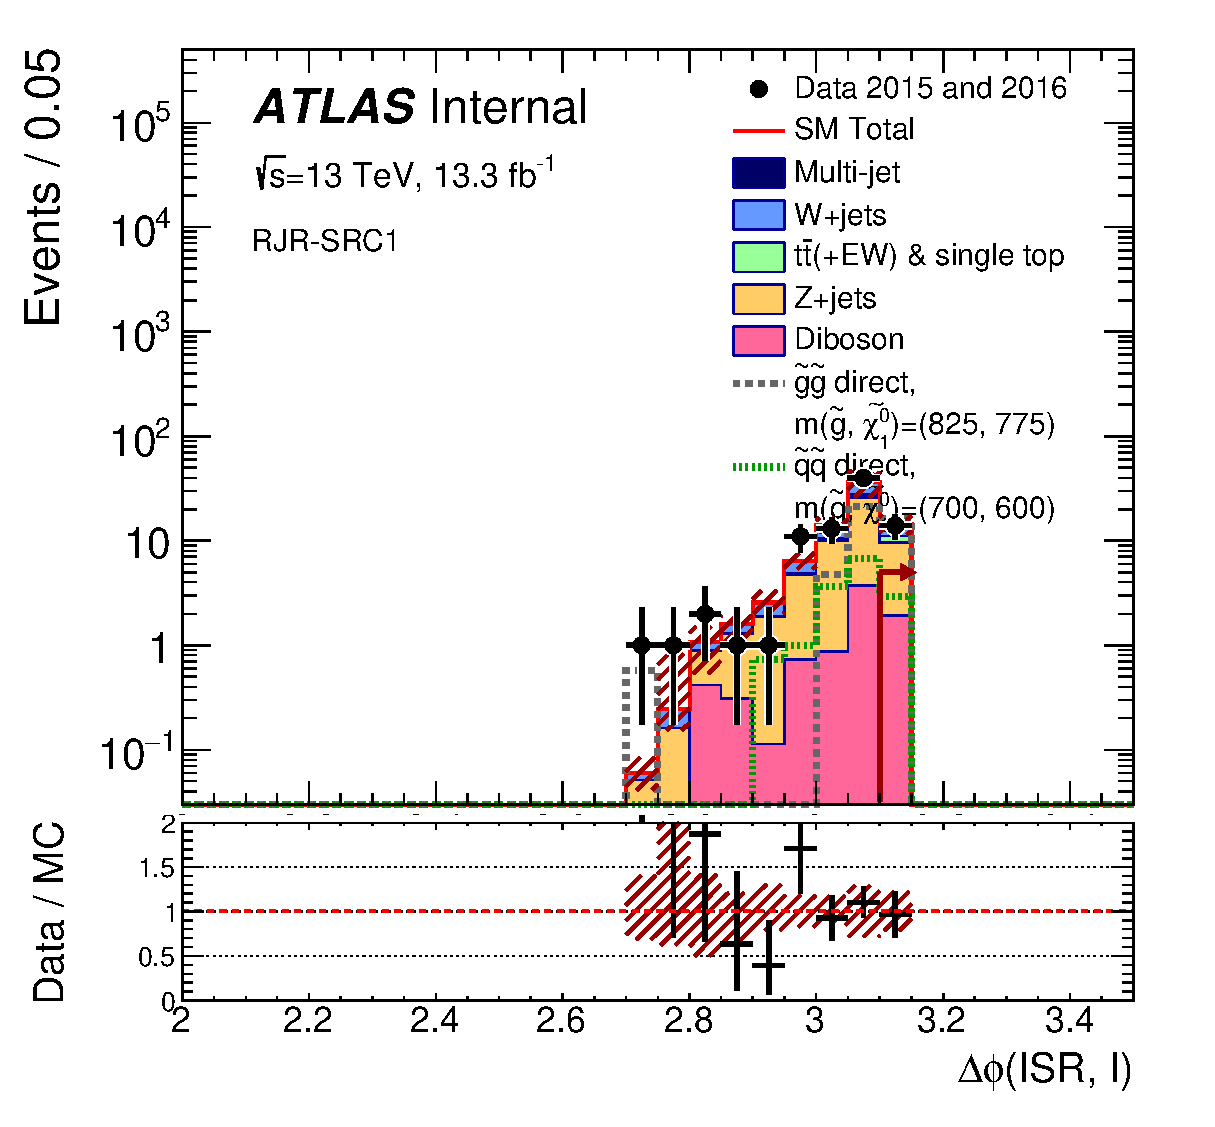
\includegraphics[width=0.33\textwidth]{ATLAS-CONF-2016-078_INT/N-1Plots/AtlasStyle/SR_SRJigsawSRC1_dphiISRI_SR_minusone}
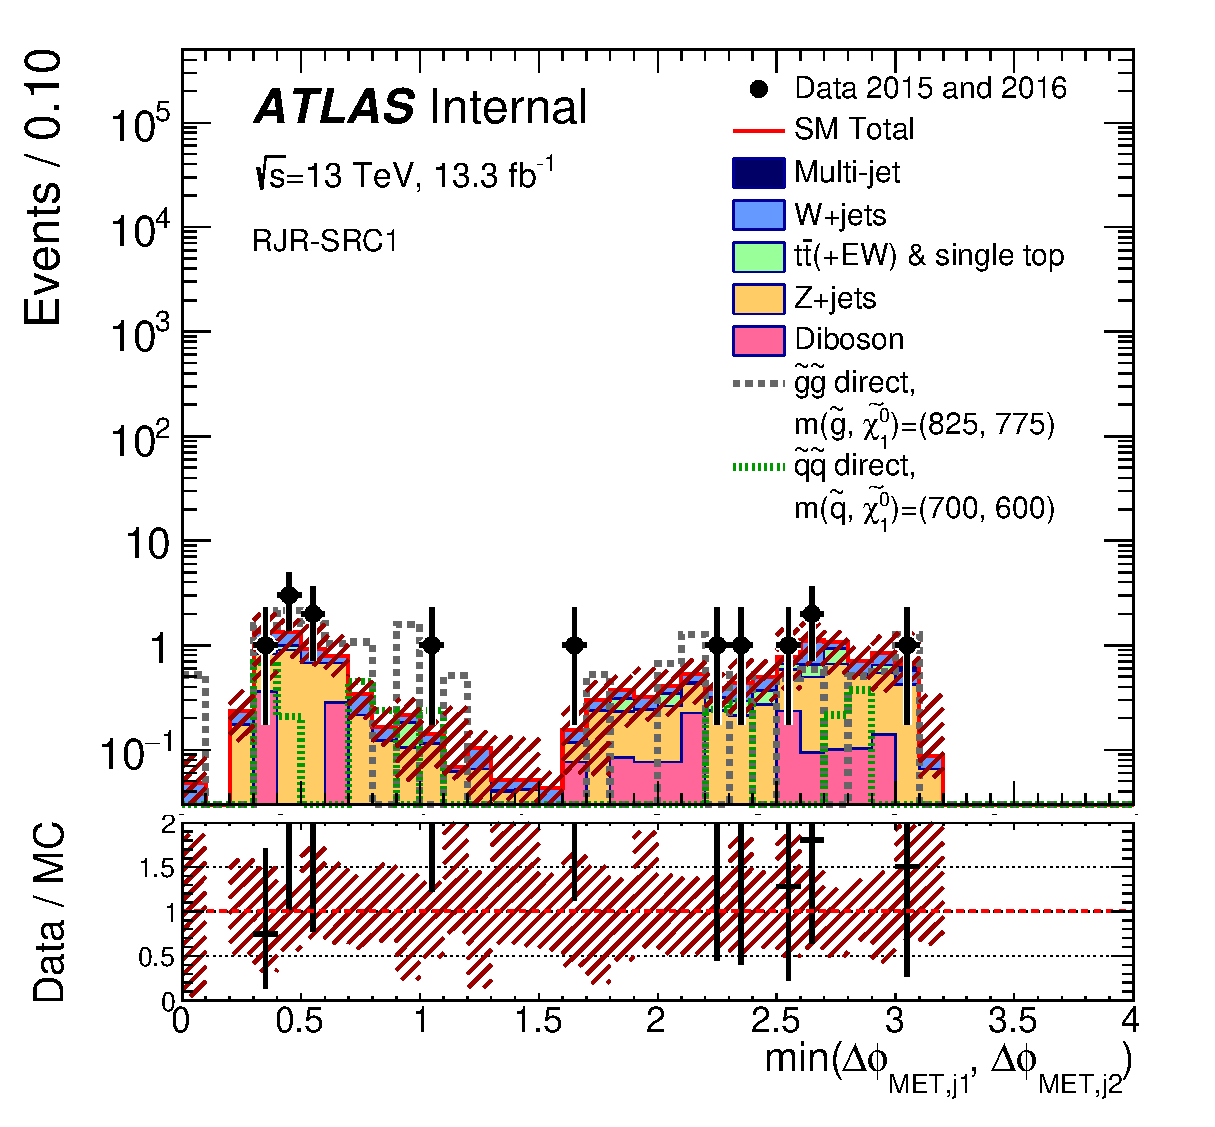
\includegraphics[width=0.33\textwidth]{ATLAS-CONF-2016-078_INT/N-1Plots/AtlasStyle/SR_SRJigsawSRC1_dphiMin2_SR_minusone}
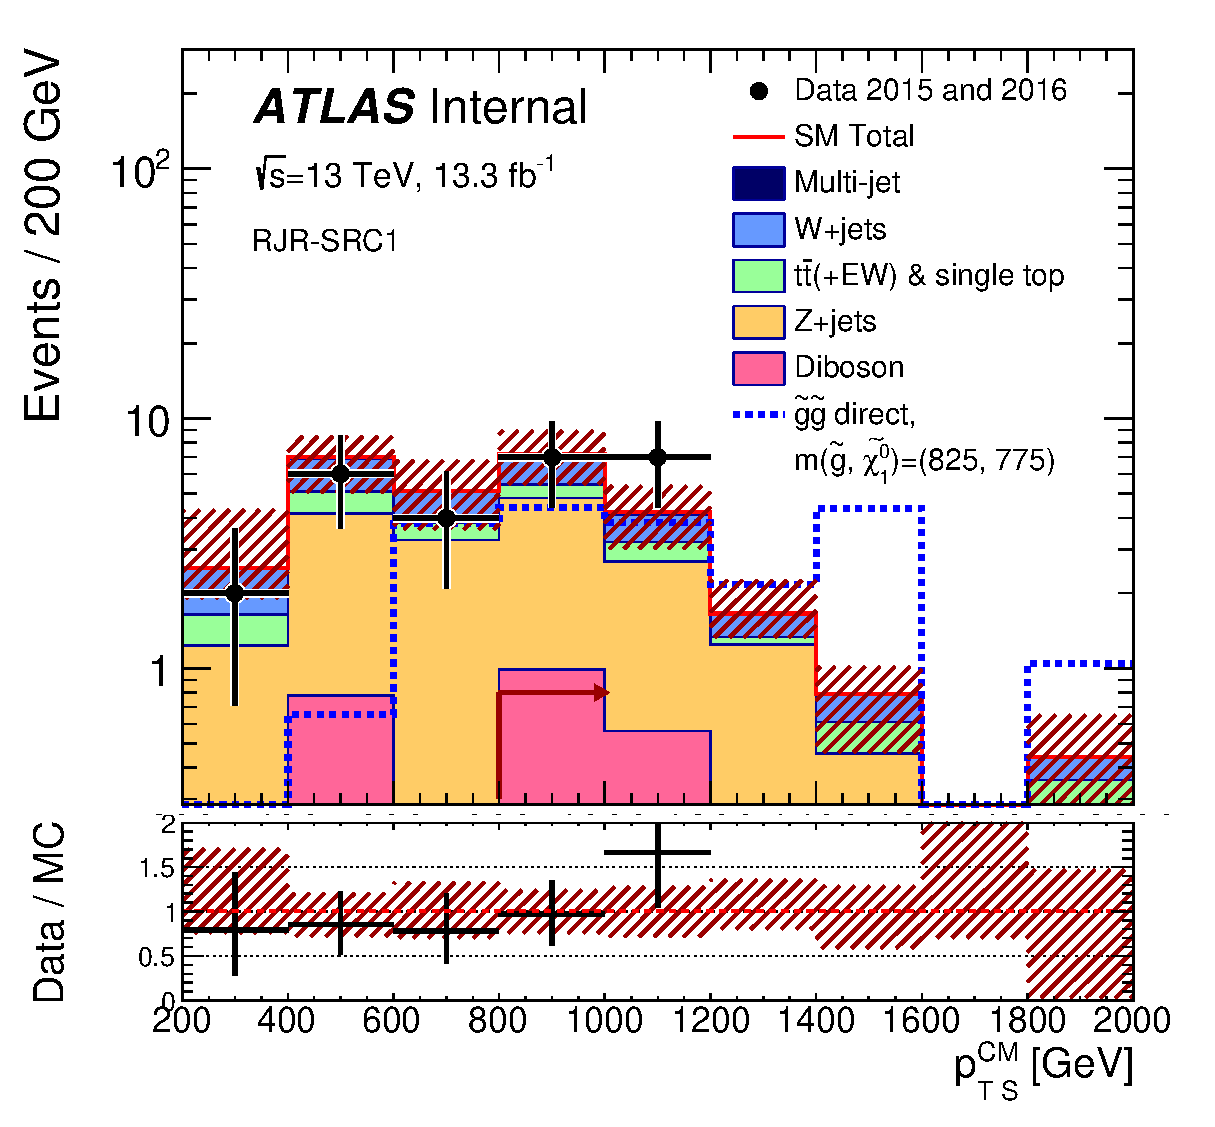
\includegraphics[width=0.33\textwidth]{ATLAS-CONF-2016-078_INT/N-1Plots/AtlasStyle/SR_SRJigsawSRC1_LastCut_SR_minusone}
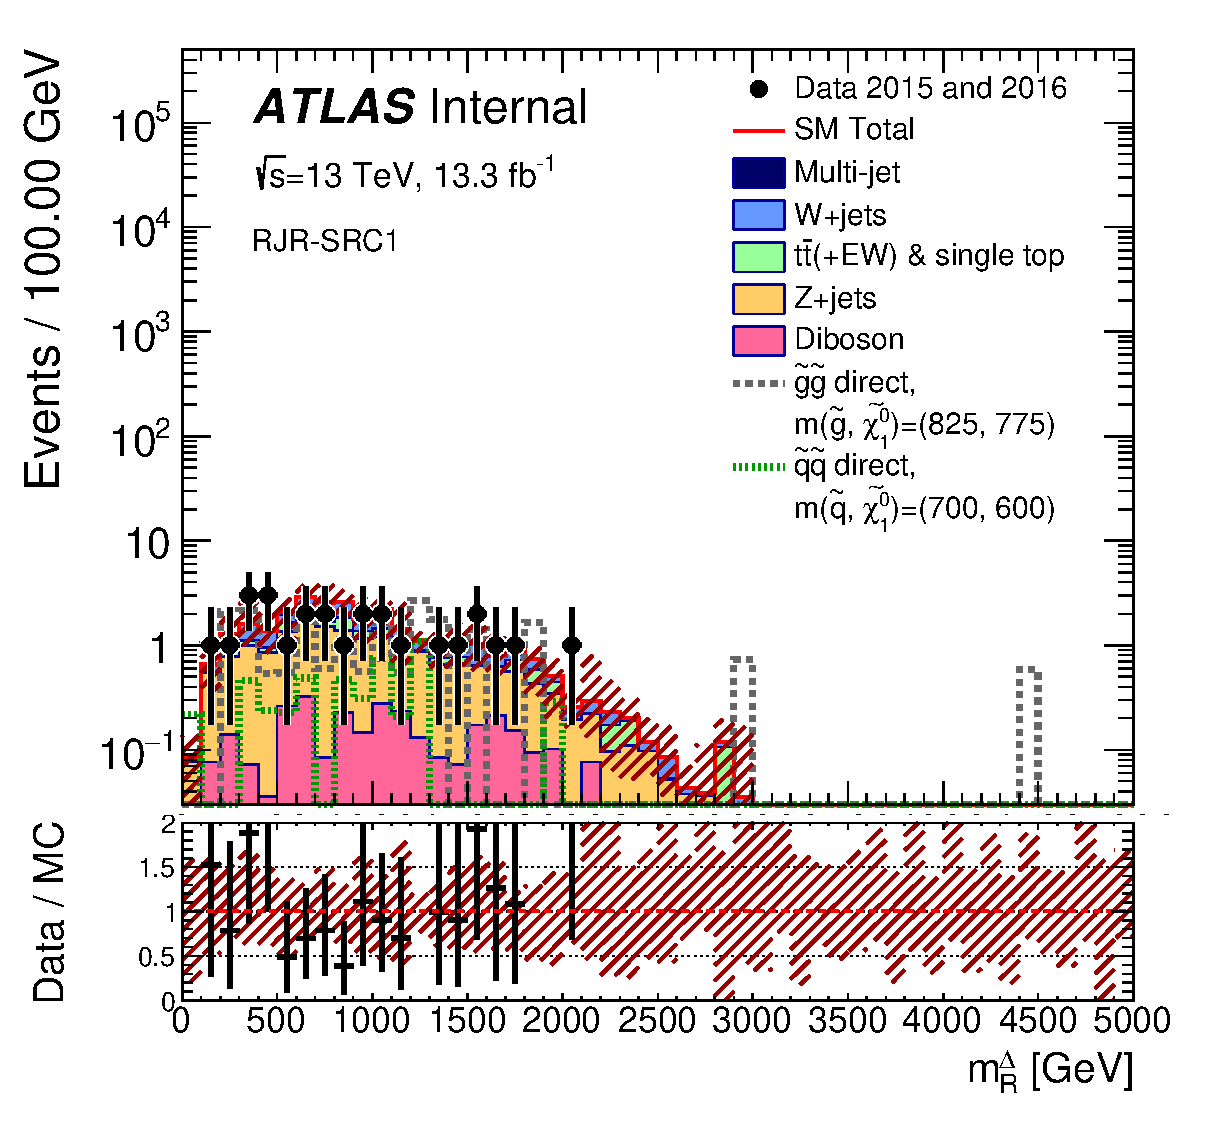
\includegraphics[width=0.33\textwidth]{ATLAS-CONF-2016-078_INT/N-1Plots/AtlasStyle/SR_SRJigsawSRC1_mDR_SR_minusone}
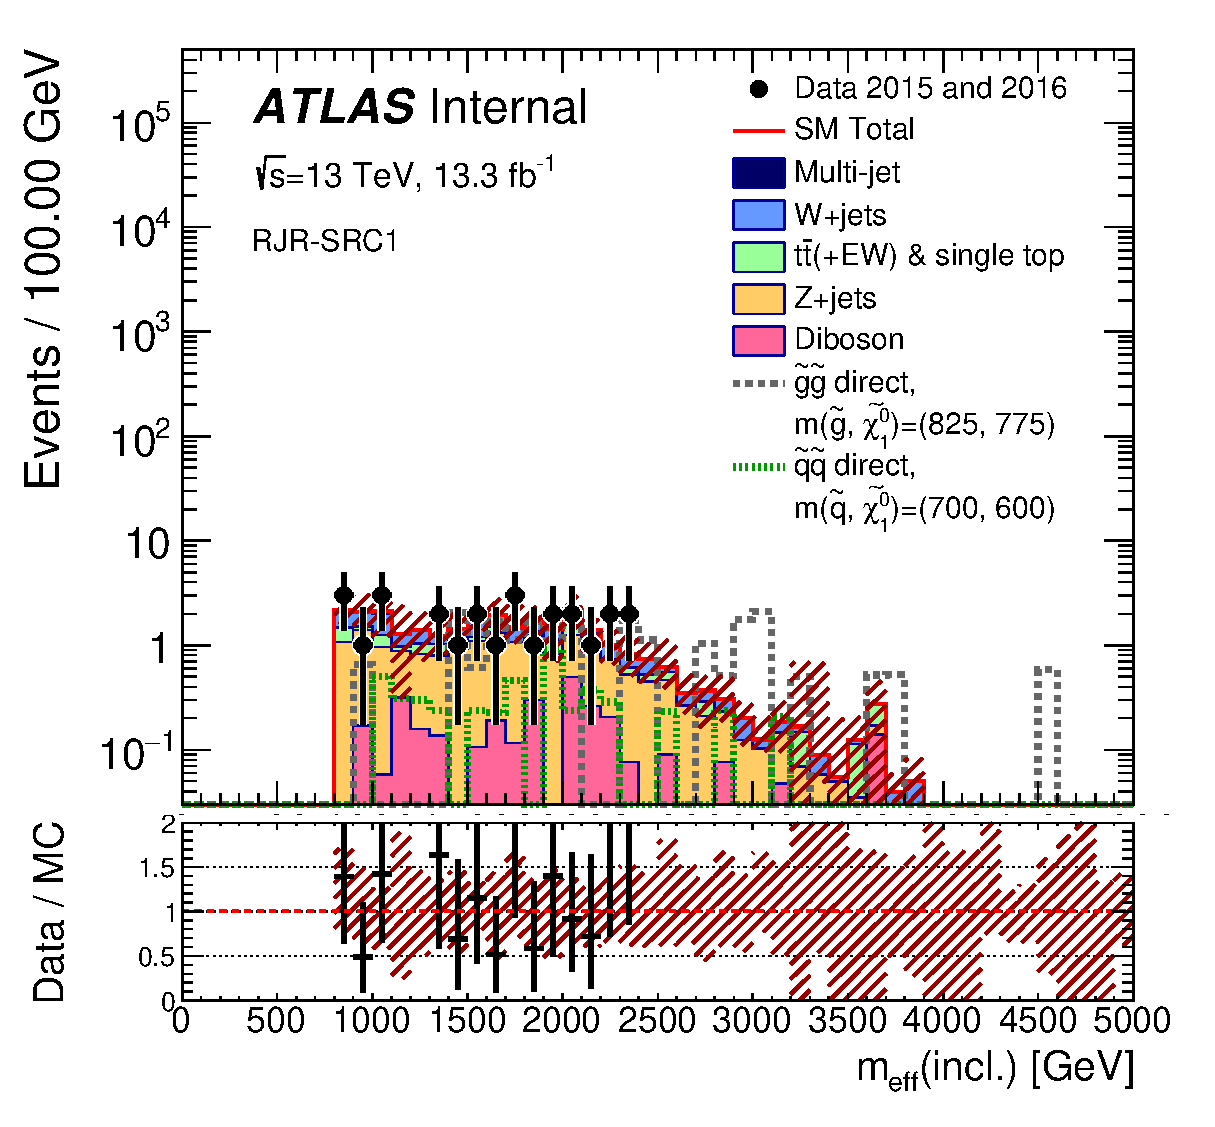
\includegraphics[width=0.33\textwidth]{ATLAS-CONF-2016-078_INT/N-1Plots/AtlasStyle/SR_SRJigsawSRC1_meffincl_SR_minusone}
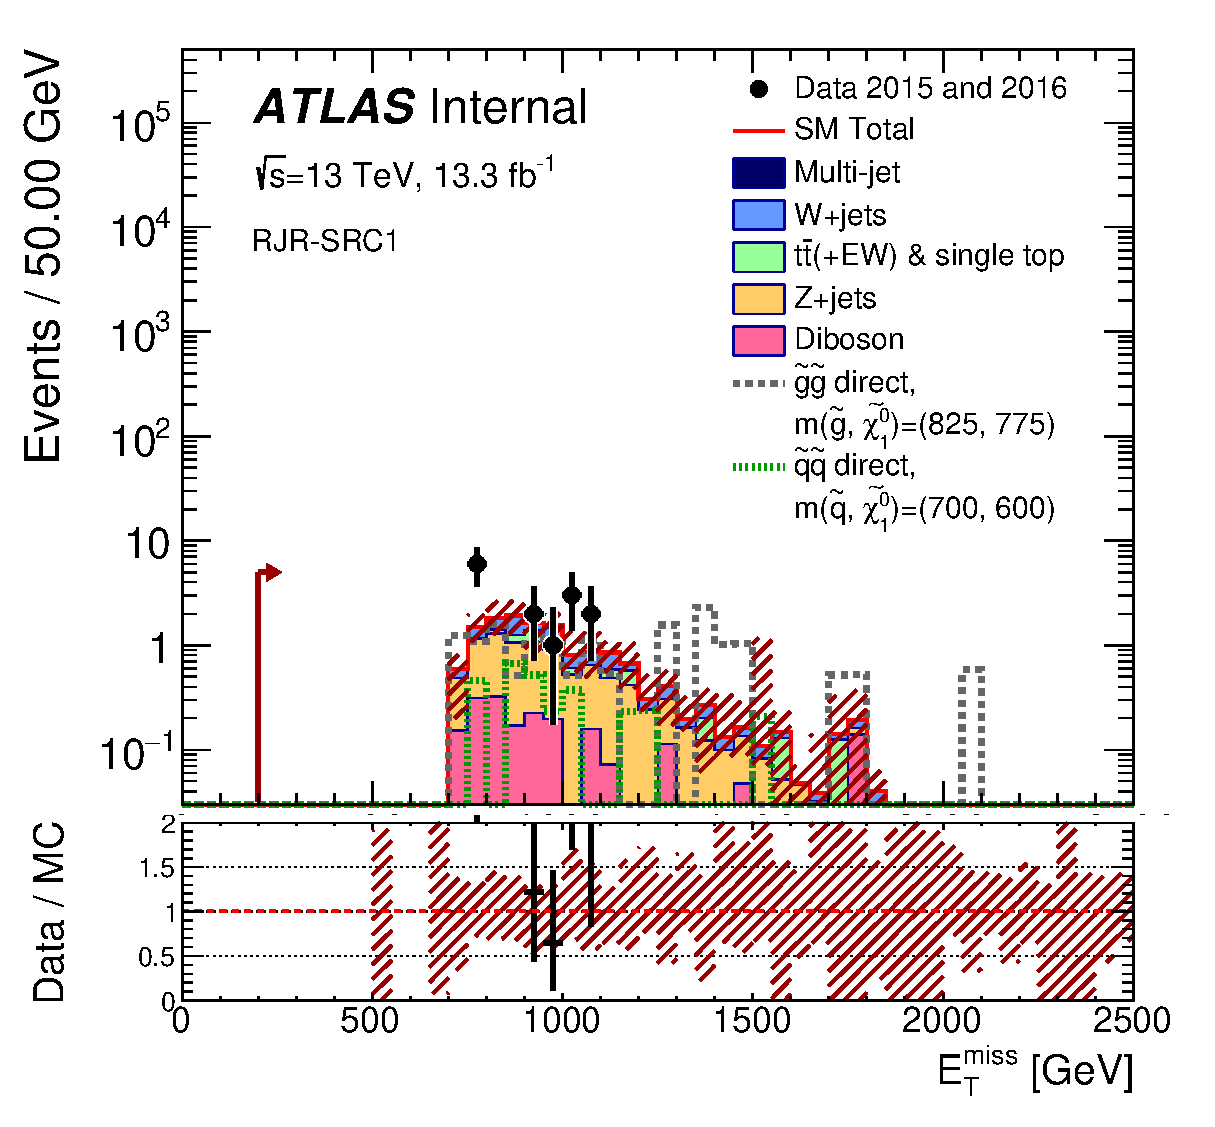
\includegraphics[width=0.33\textwidth]{ATLAS-CONF-2016-078_INT/N-1Plots/AtlasStyle/SR_SRJigsawSRC1_met_SR_minusone}
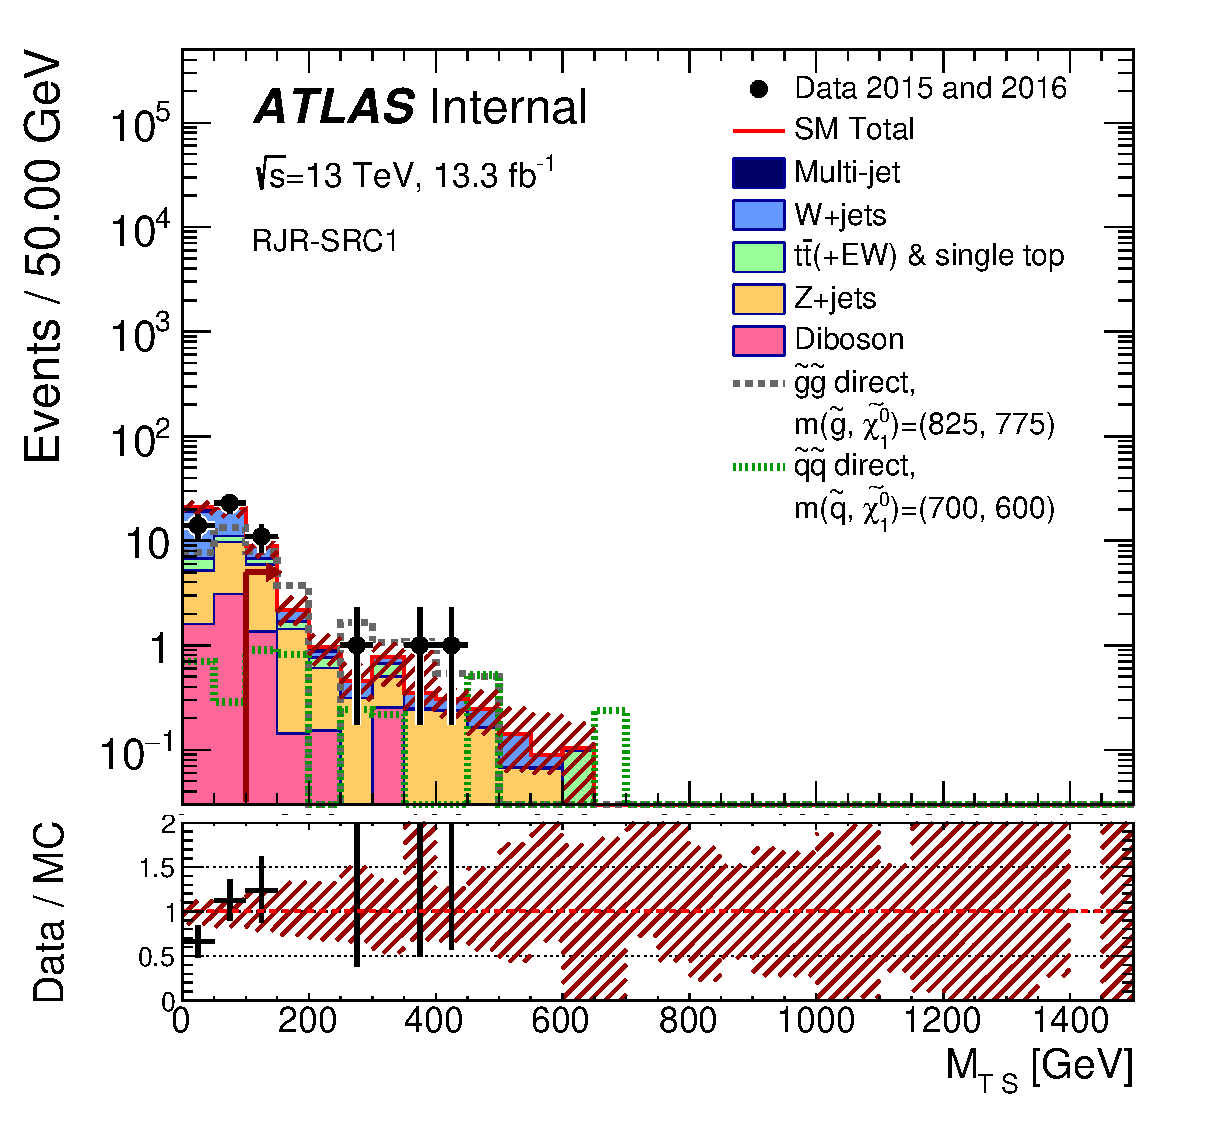
\includegraphics[width=0.33\textwidth]{ATLAS-CONF-2016-078_INT/N-1Plots/AtlasStyle/SR_SRJigsawSRC1_MS_SR_minusone}
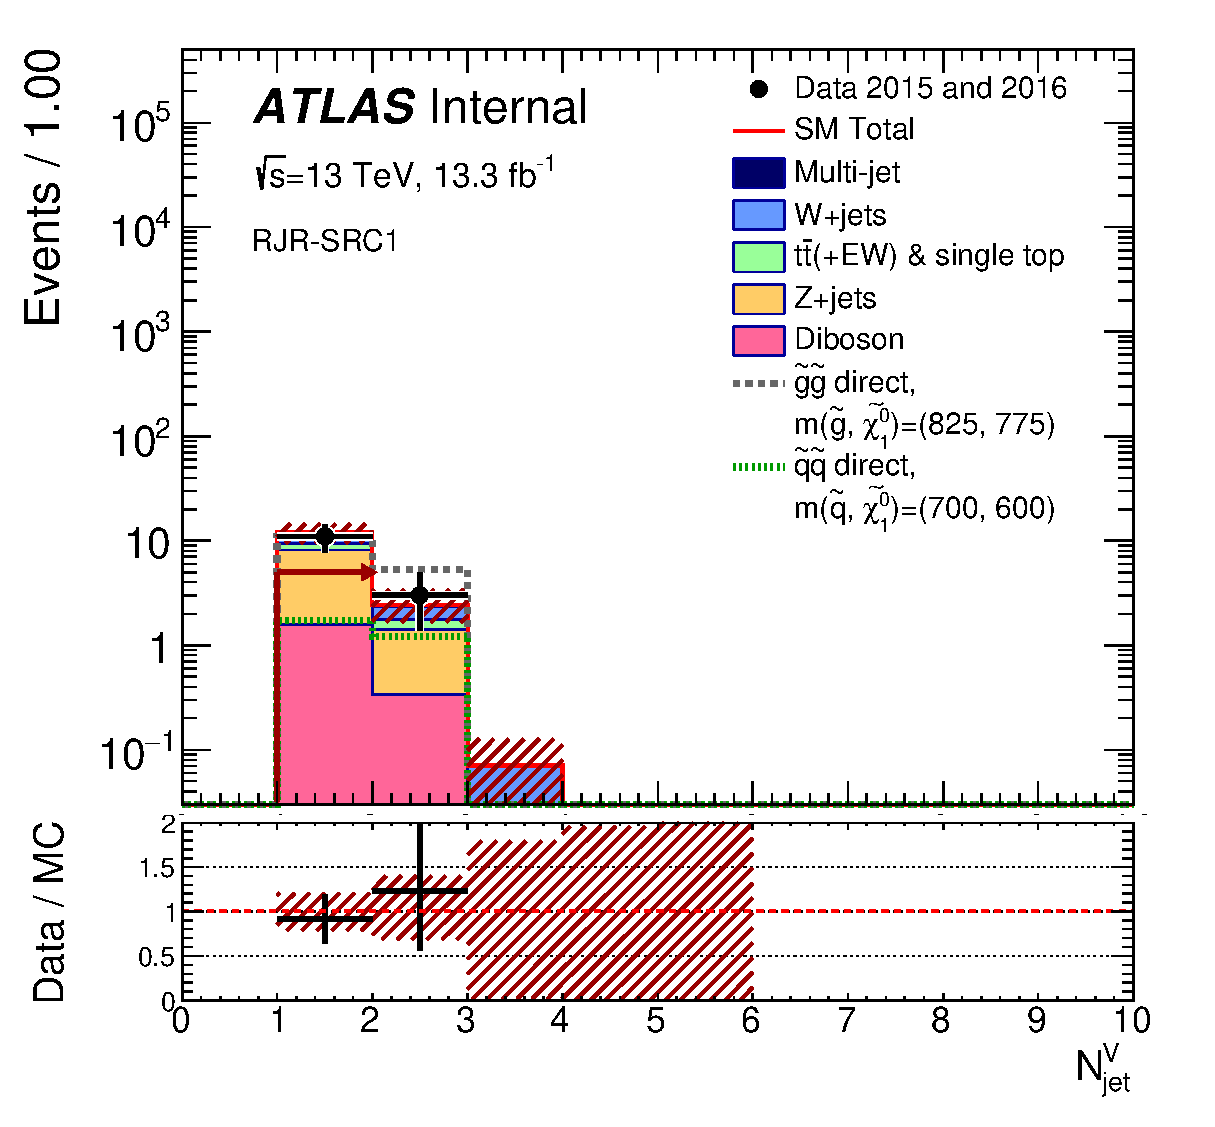
\includegraphics[width=0.33\textwidth]{ATLAS-CONF-2016-078_INT/N-1Plots/AtlasStyle/SR_SRJigsawSRC1_NV_SR_minusone}
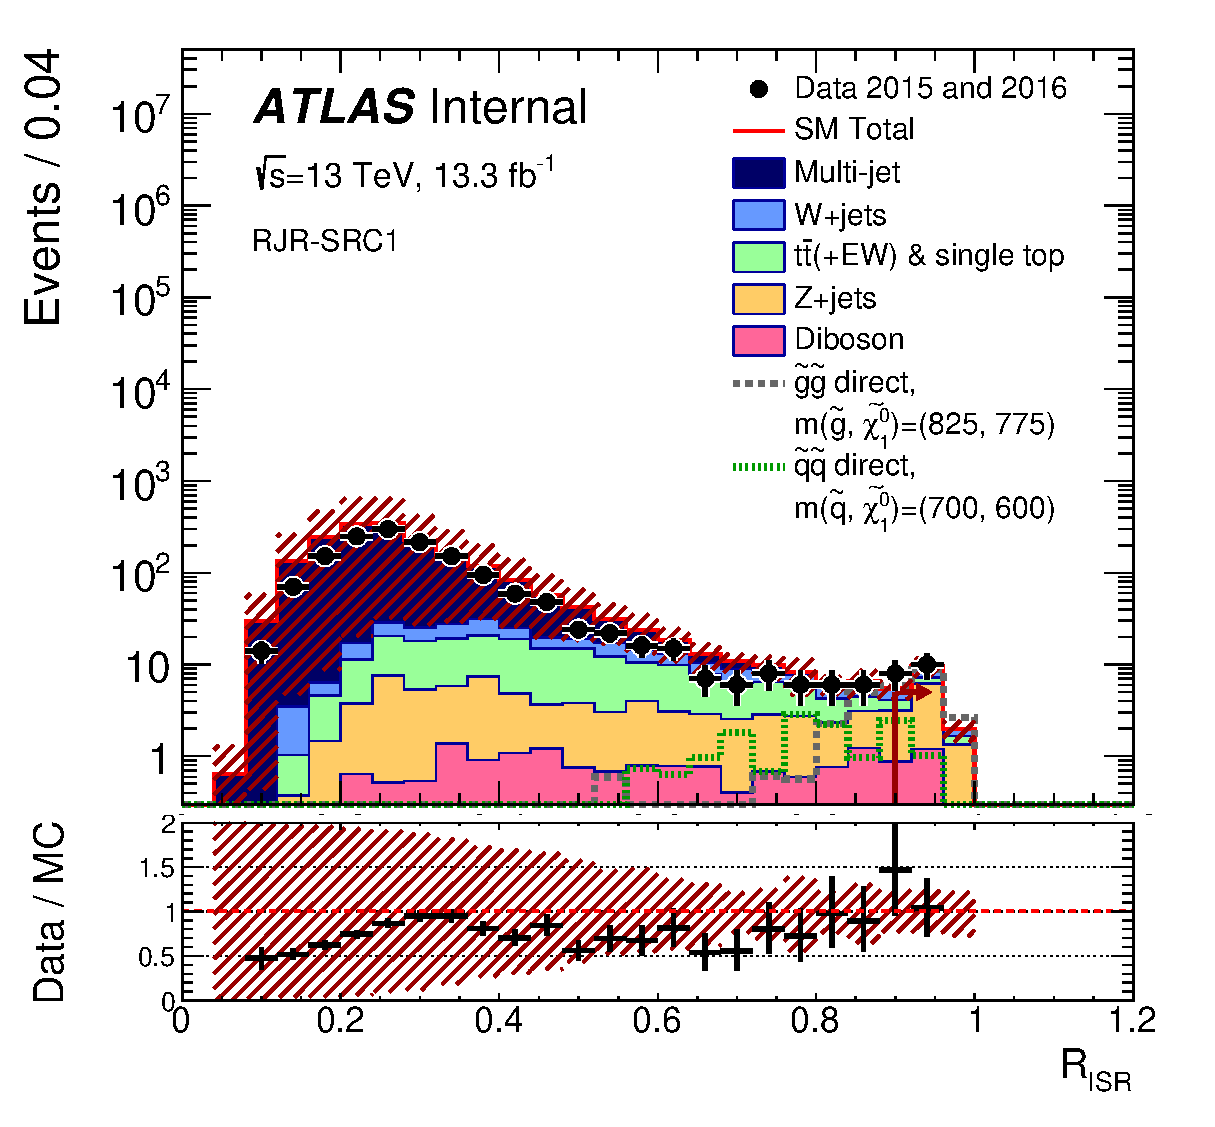
\includegraphics[width=0.33\textwidth]{ATLAS-CONF-2016-078_INT/N-1Plots/AtlasStyle/SR_SRJigsawSRC1_Ratio_SR_minusone}
\end{center}
\caption{}
\label{fig:SR_SRJigsawSRC1_deltaQCD_SR_minusone}
\end{figure}

\begin{figure}[tbph]
\begin{center}
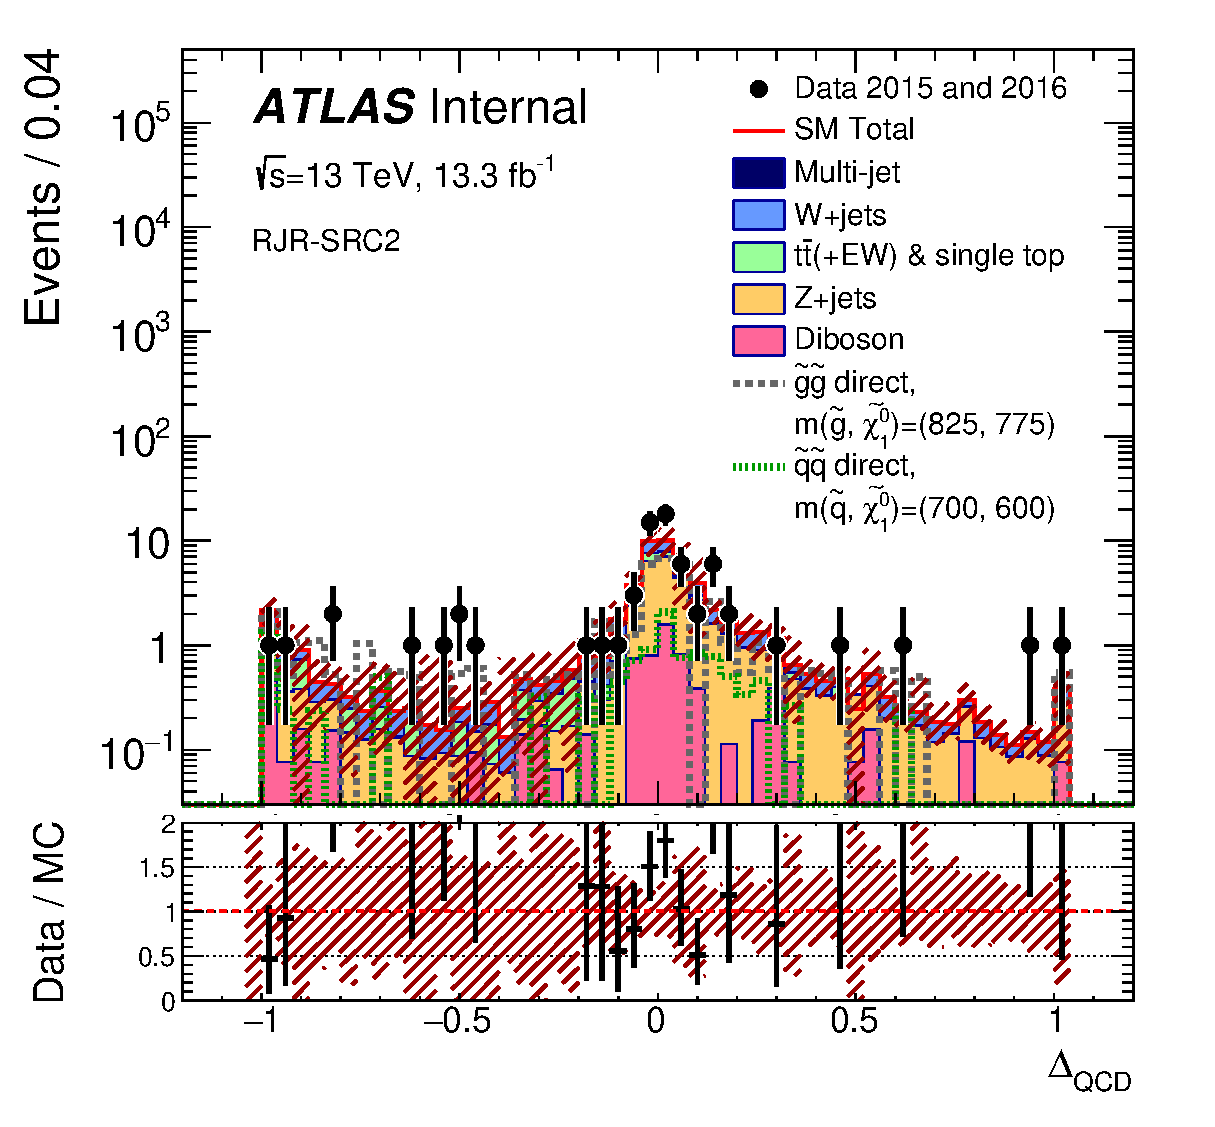
\includegraphics[width=0.33\textwidth]{ATLAS-CONF-2016-078_INT/N-1Plots/AtlasStyle/SR_SRJigsawSRC2_deltaQCD_SR_minusone}
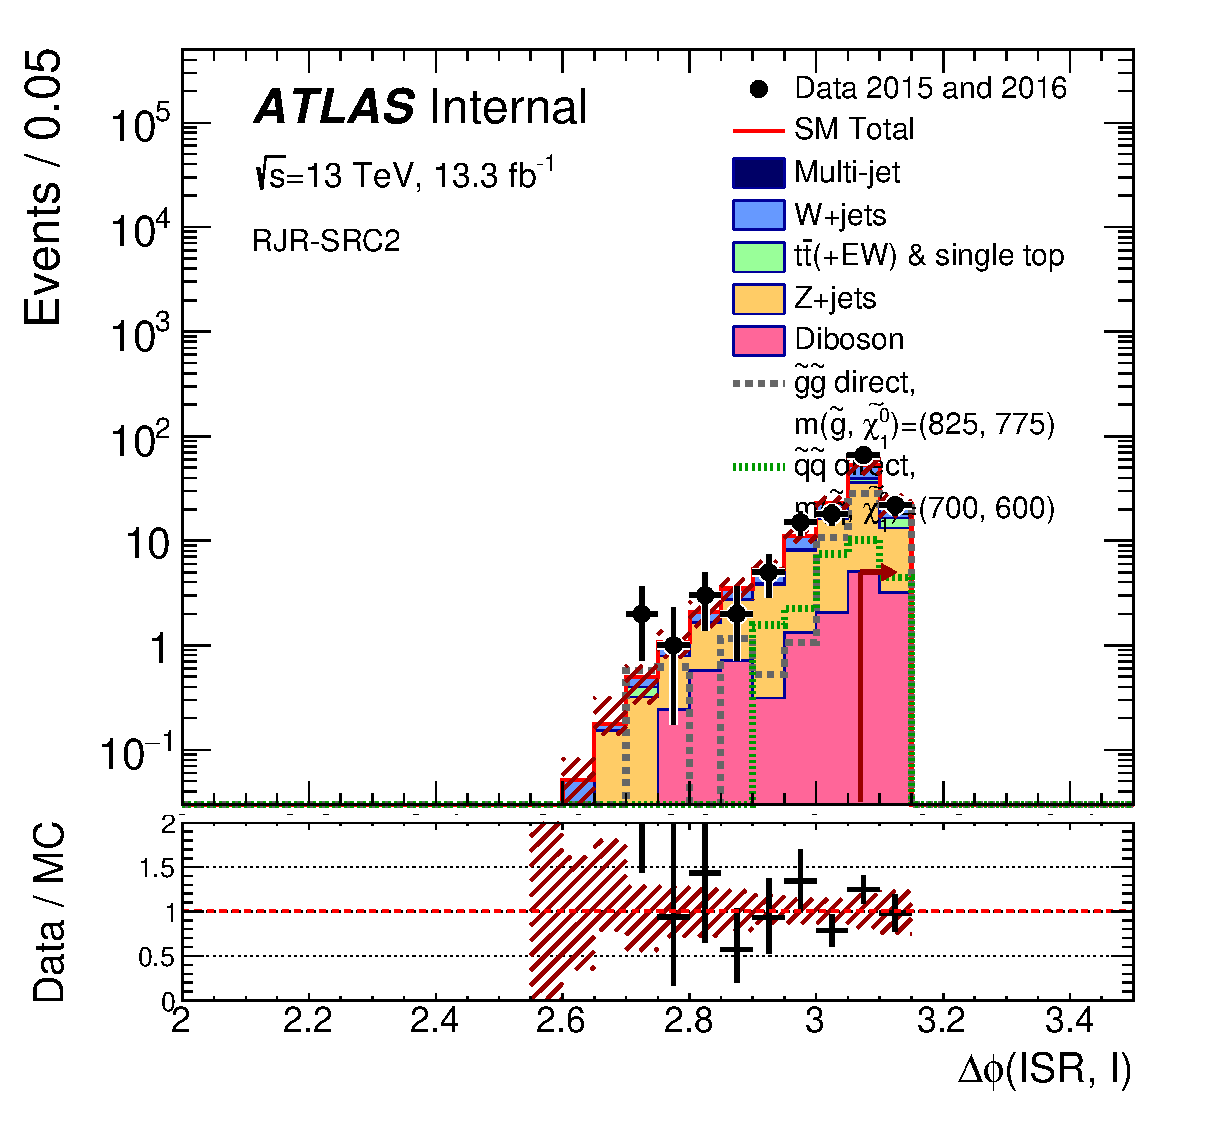
\includegraphics[width=0.33\textwidth]{ATLAS-CONF-2016-078_INT/N-1Plots/AtlasStyle/SR_SRJigsawSRC2_dphiISRI_SR_minusone}
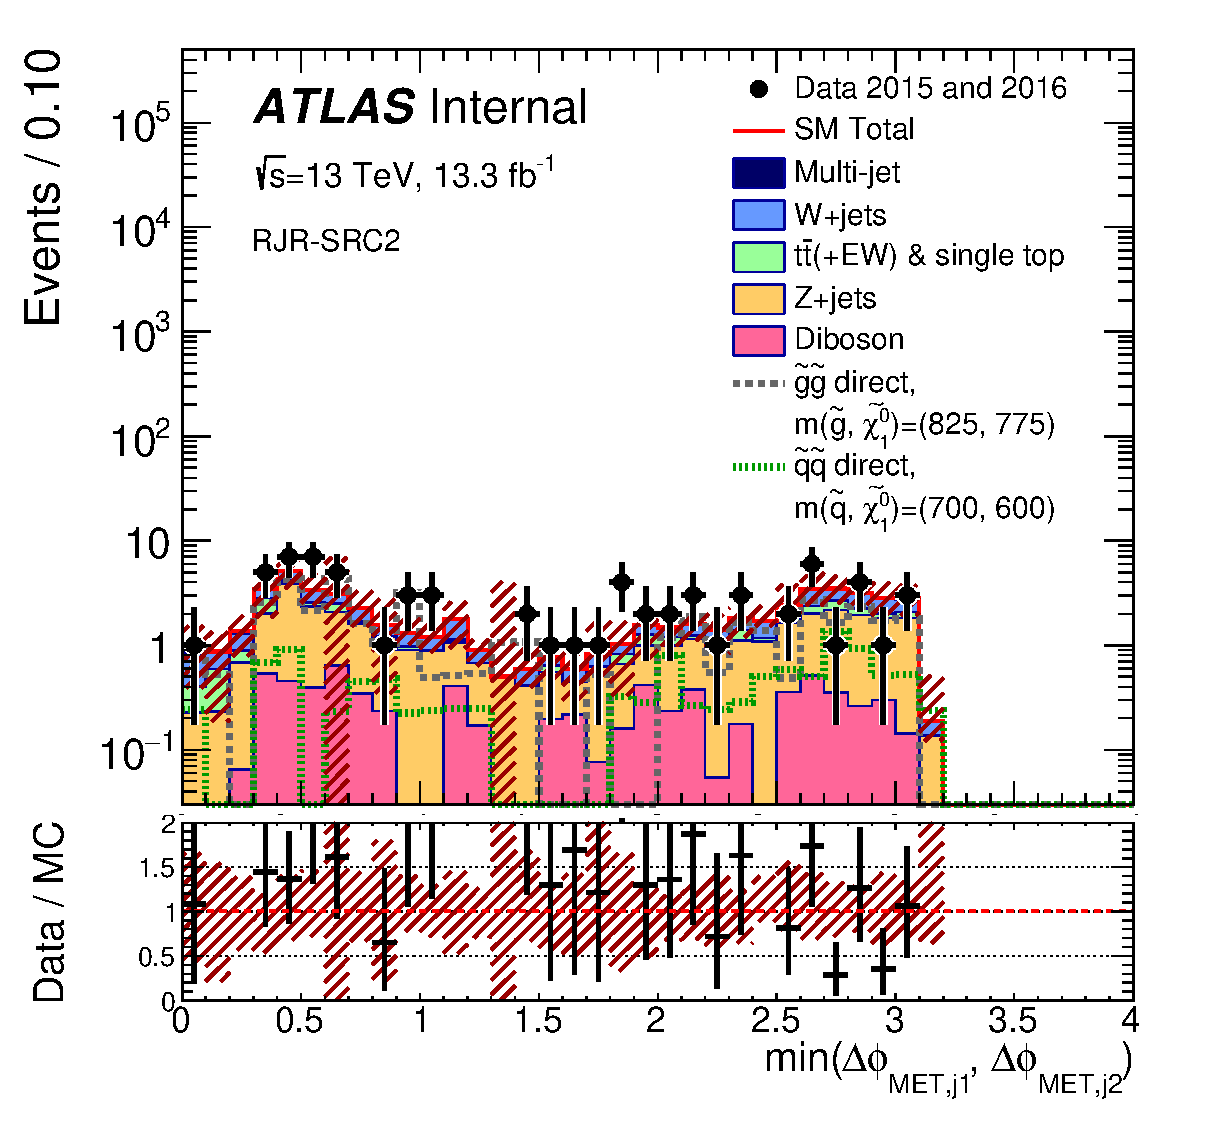
\includegraphics[width=0.33\textwidth]{ATLAS-CONF-2016-078_INT/N-1Plots/AtlasStyle/SR_SRJigsawSRC2_dphiMin2_SR_minusone}
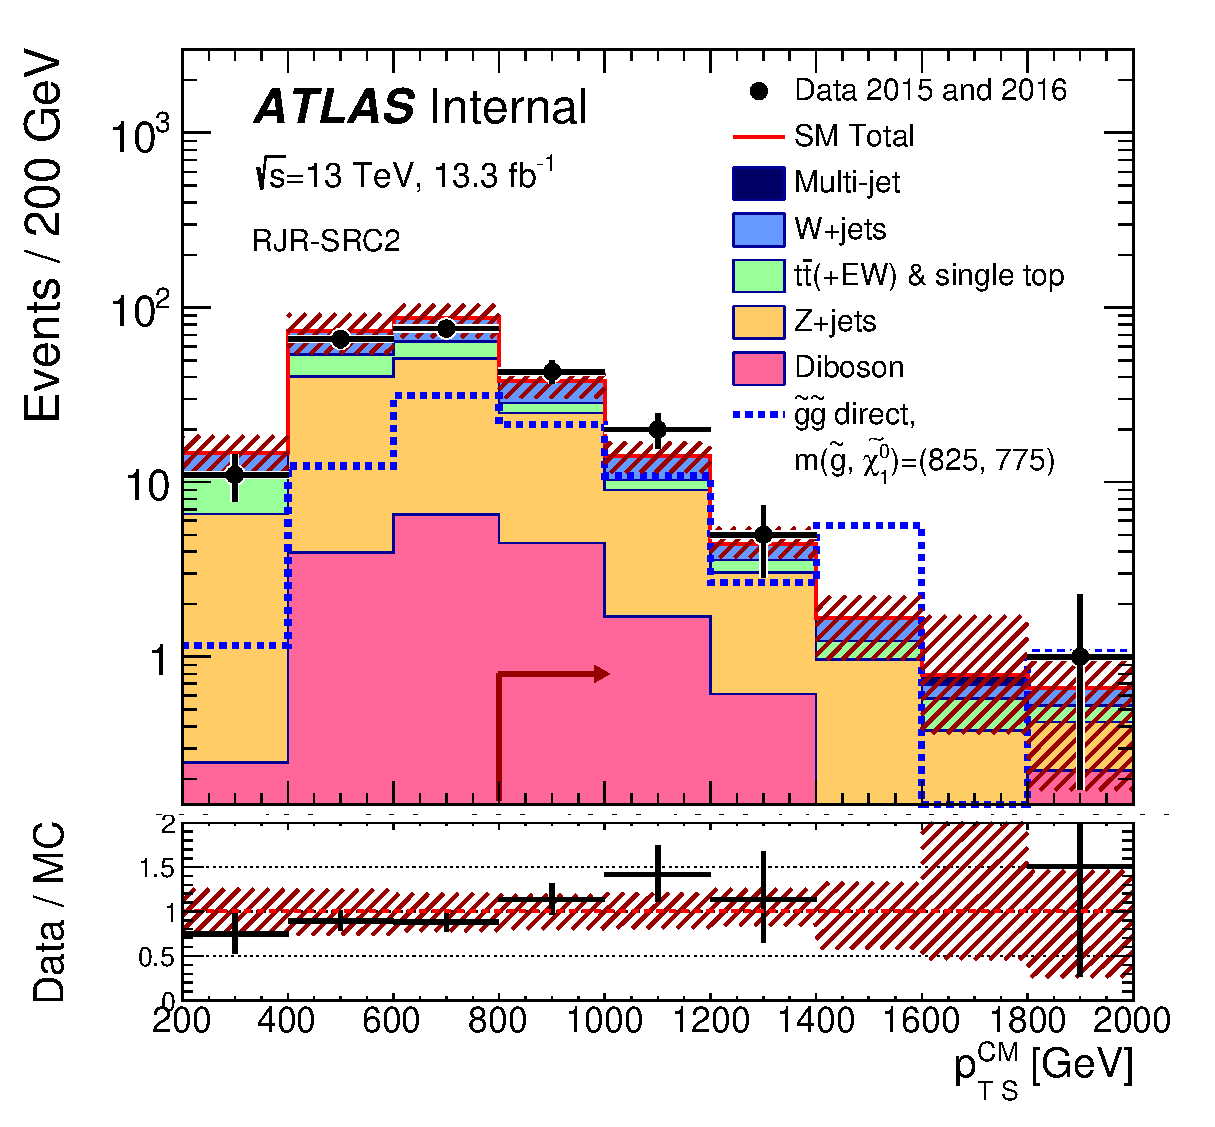
\includegraphics[width=0.33\textwidth]{ATLAS-CONF-2016-078_INT/N-1Plots/AtlasStyle/SR_SRJigsawSRC2_LastCut_SR_minusone}
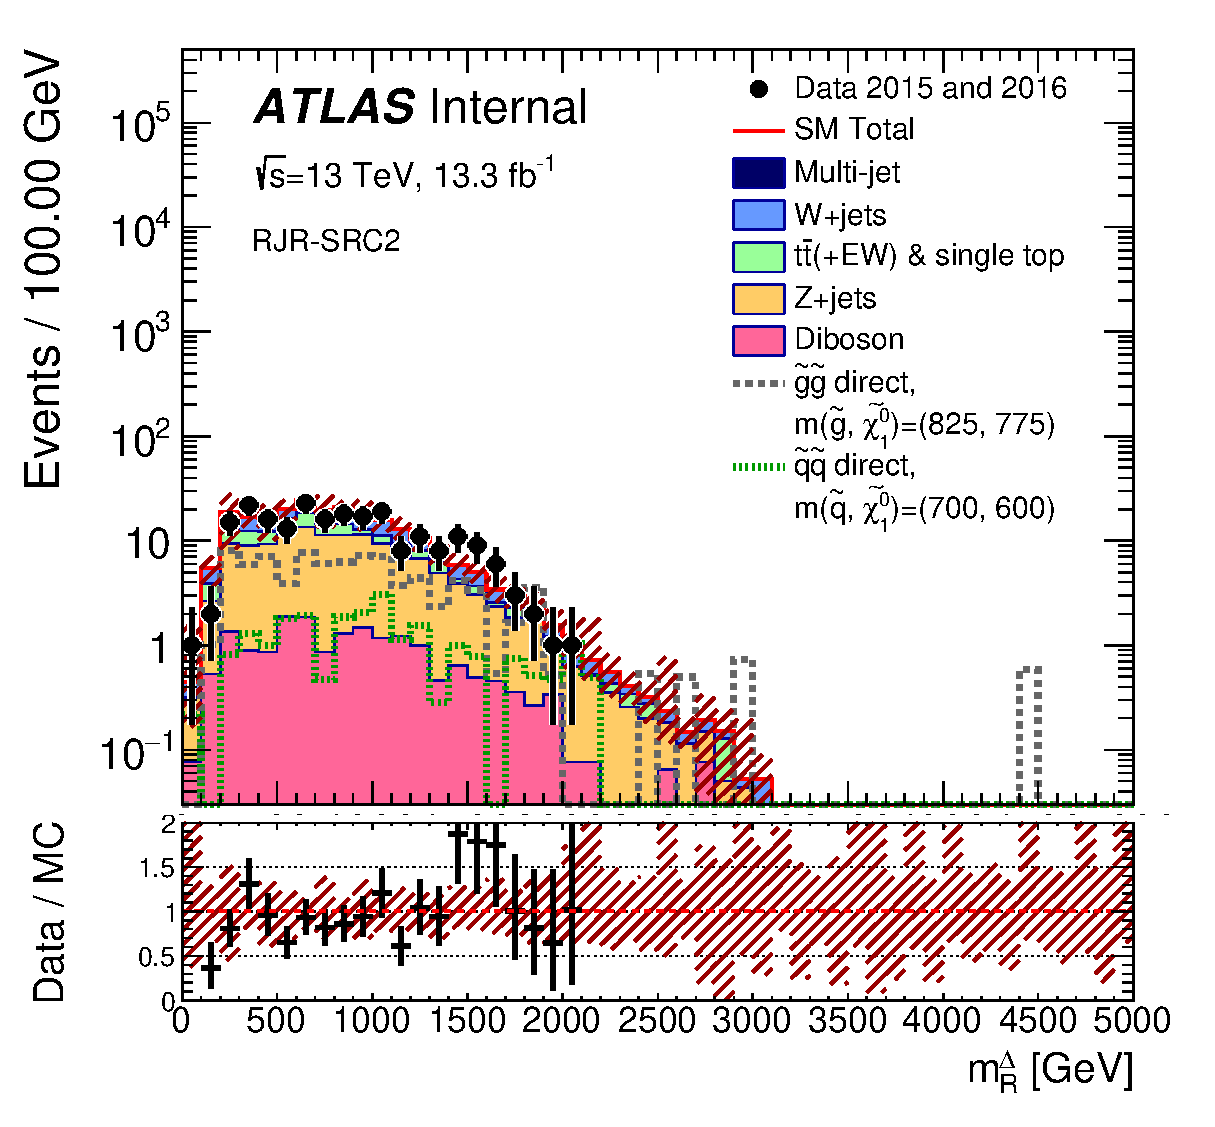
\includegraphics[width=0.33\textwidth]{ATLAS-CONF-2016-078_INT/N-1Plots/AtlasStyle/SR_SRJigsawSRC2_mDR_SR_minusone}
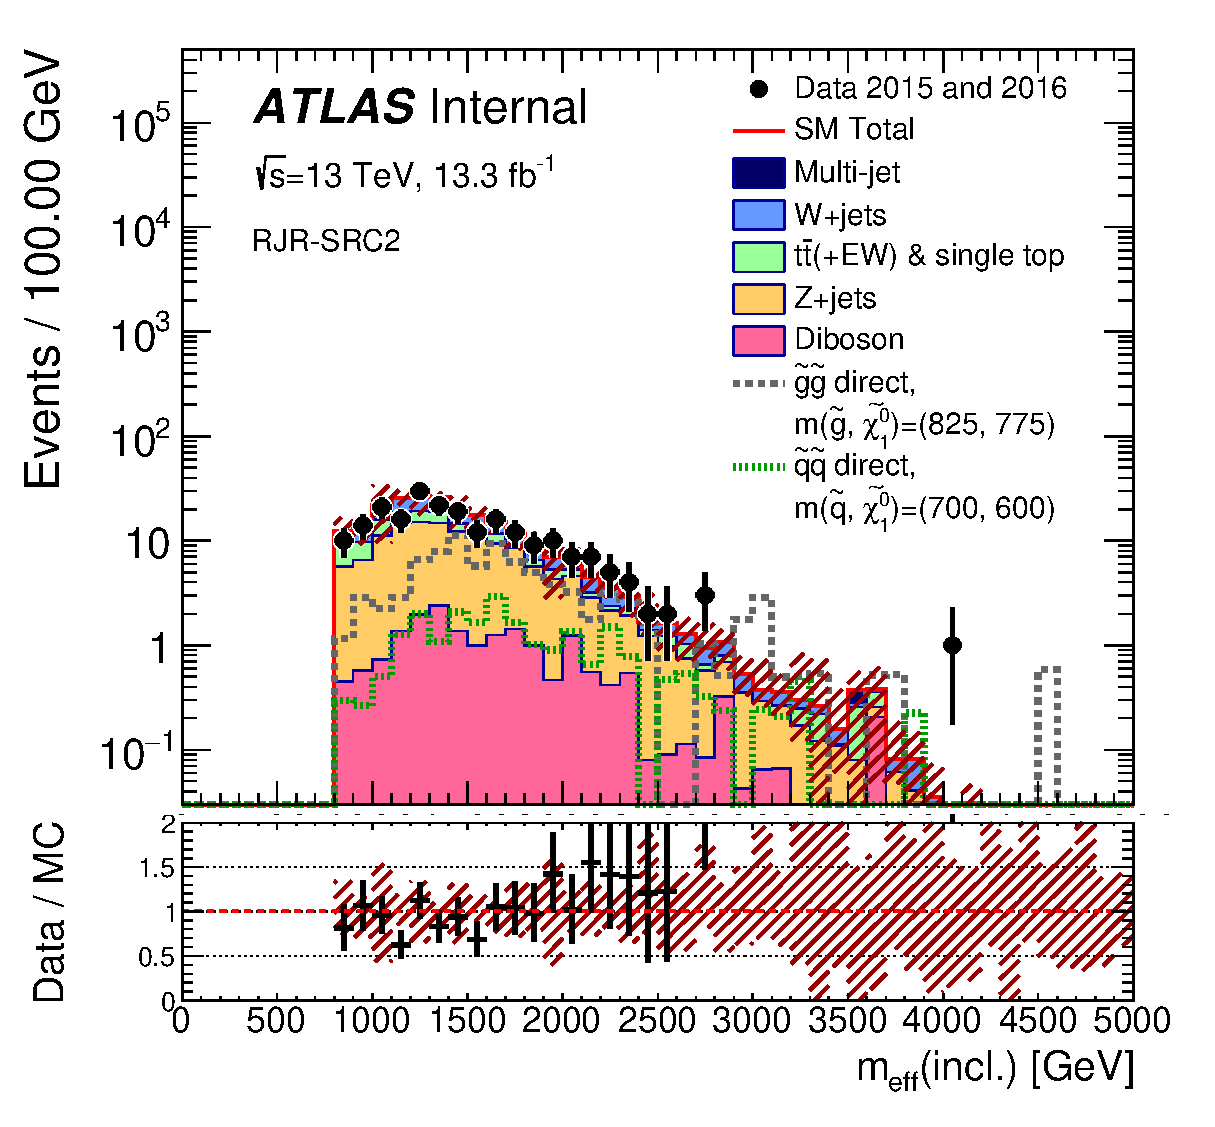
\includegraphics[width=0.33\textwidth]{ATLAS-CONF-2016-078_INT/N-1Plots/AtlasStyle/SR_SRJigsawSRC2_meffincl_SR_minusone}
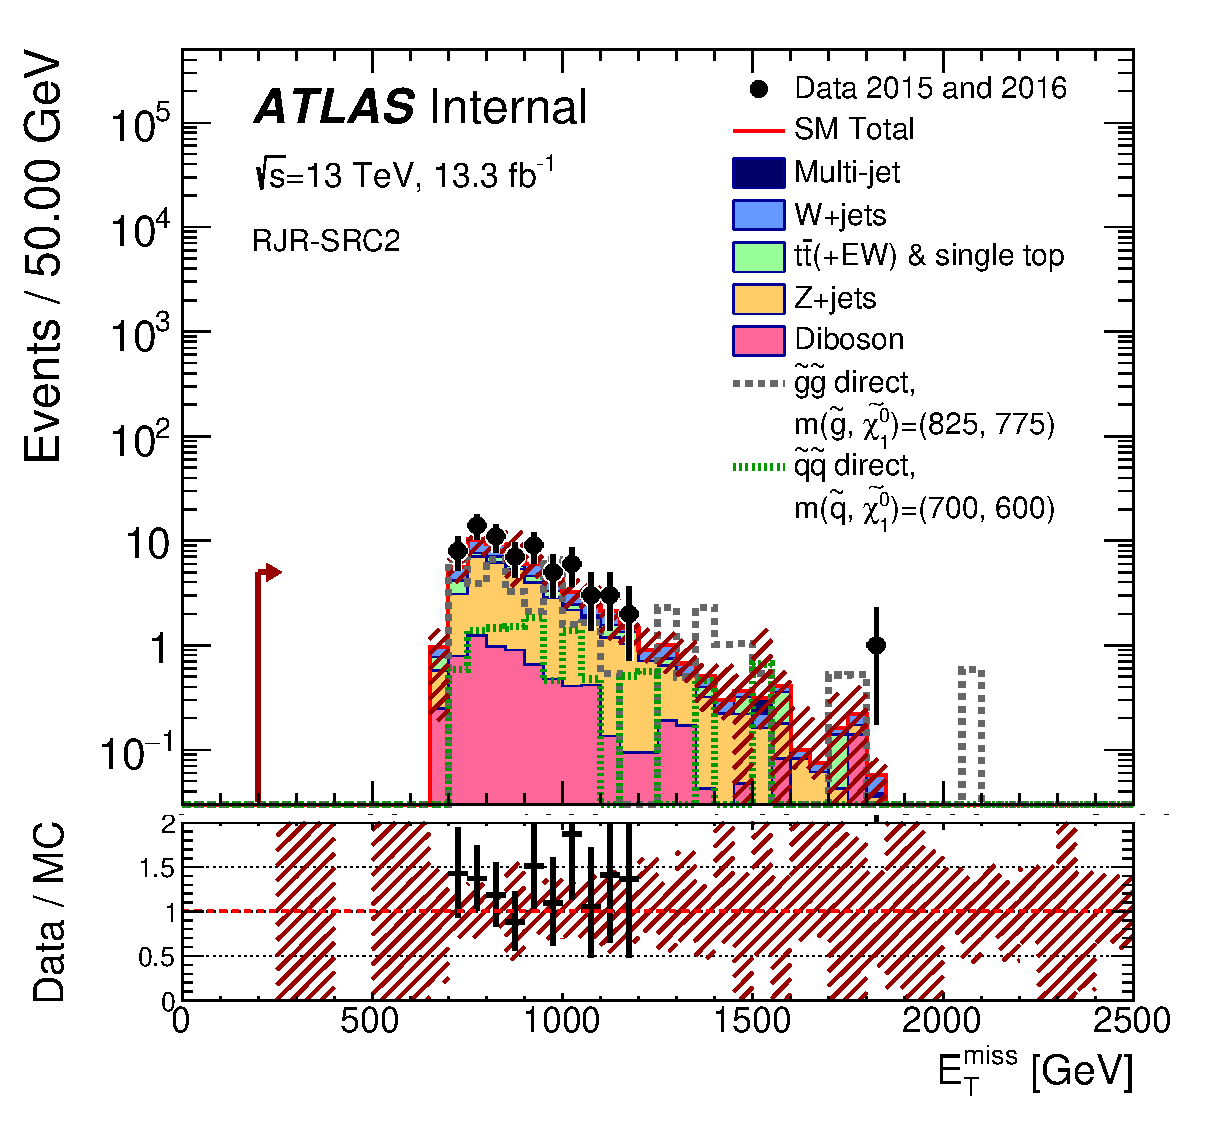
\includegraphics[width=0.33\textwidth]{ATLAS-CONF-2016-078_INT/N-1Plots/AtlasStyle/SR_SRJigsawSRC2_met_SR_minusone}
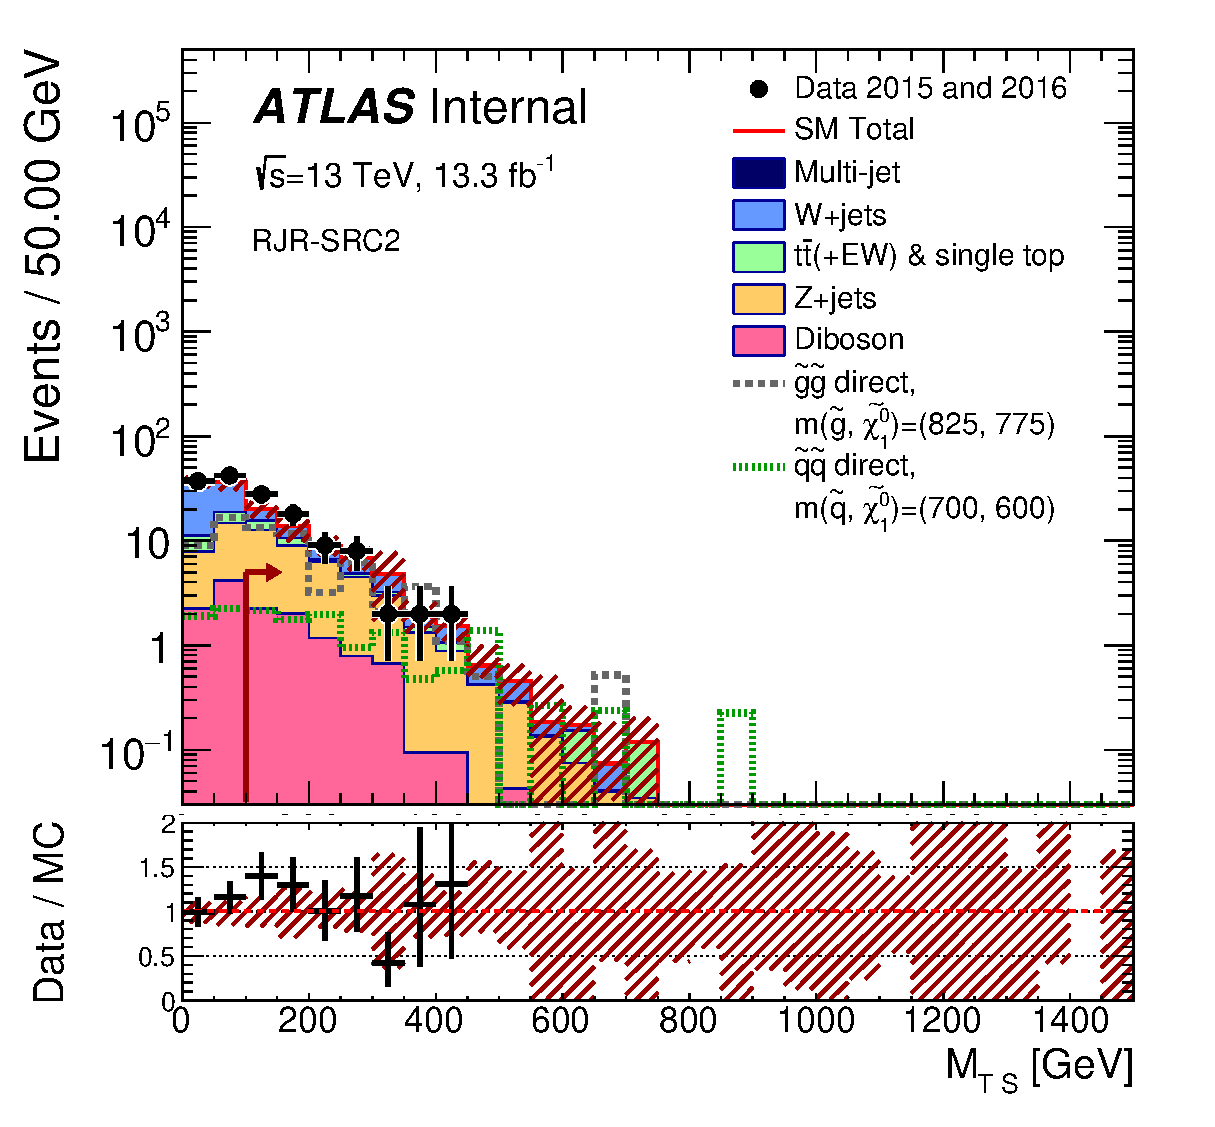
\includegraphics[width=0.33\textwidth]{ATLAS-CONF-2016-078_INT/N-1Plots/AtlasStyle/SR_SRJigsawSRC2_MS_SR_minusone}
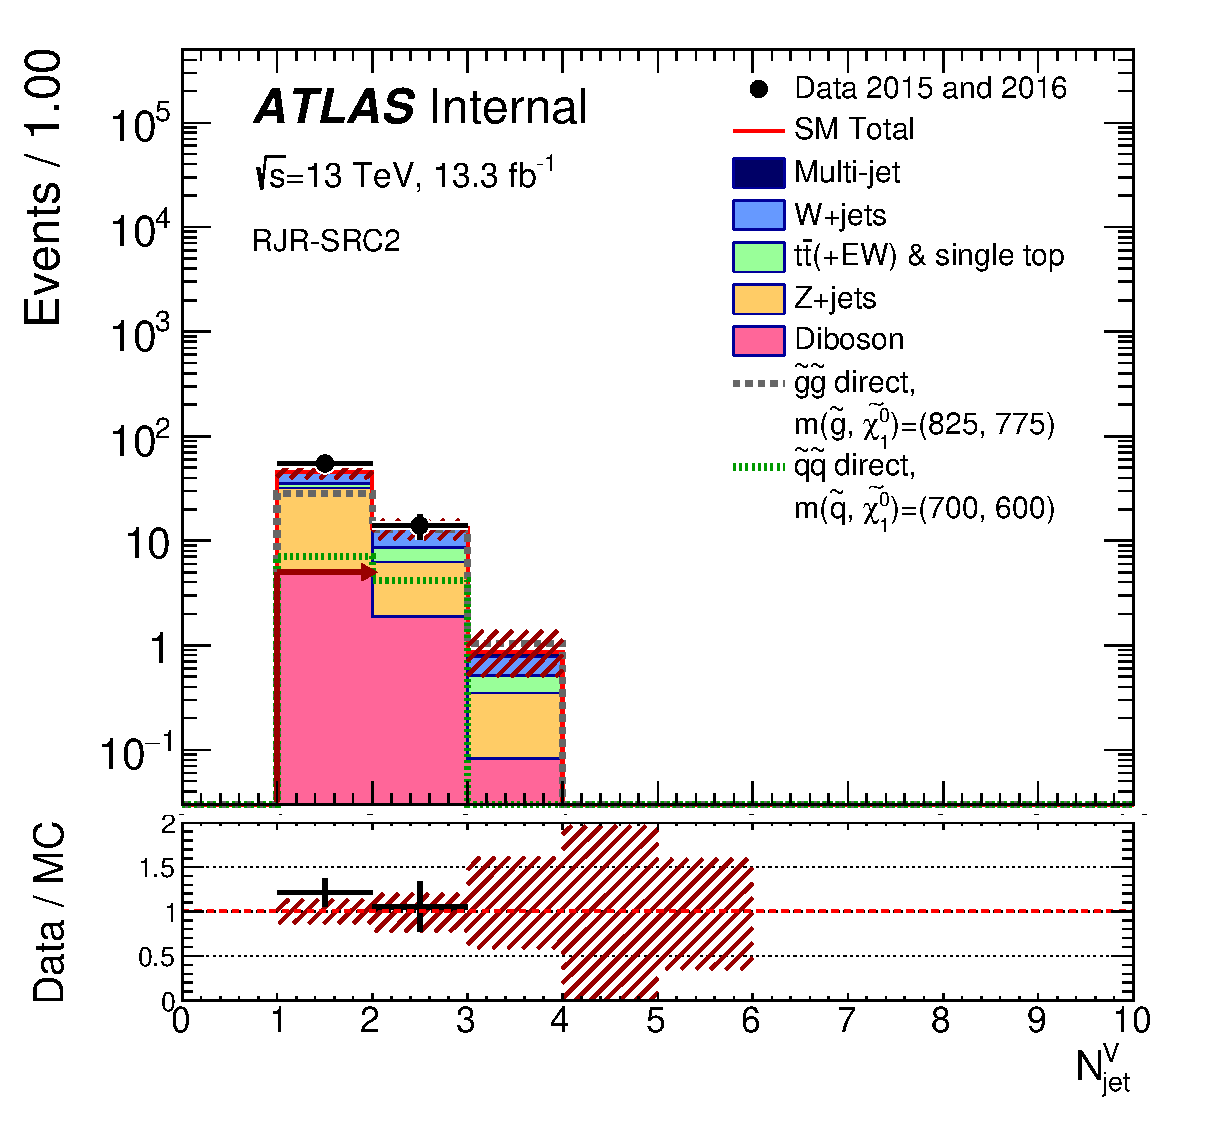
\includegraphics[width=0.33\textwidth]{ATLAS-CONF-2016-078_INT/N-1Plots/AtlasStyle/SR_SRJigsawSRC2_NV_SR_minusone}
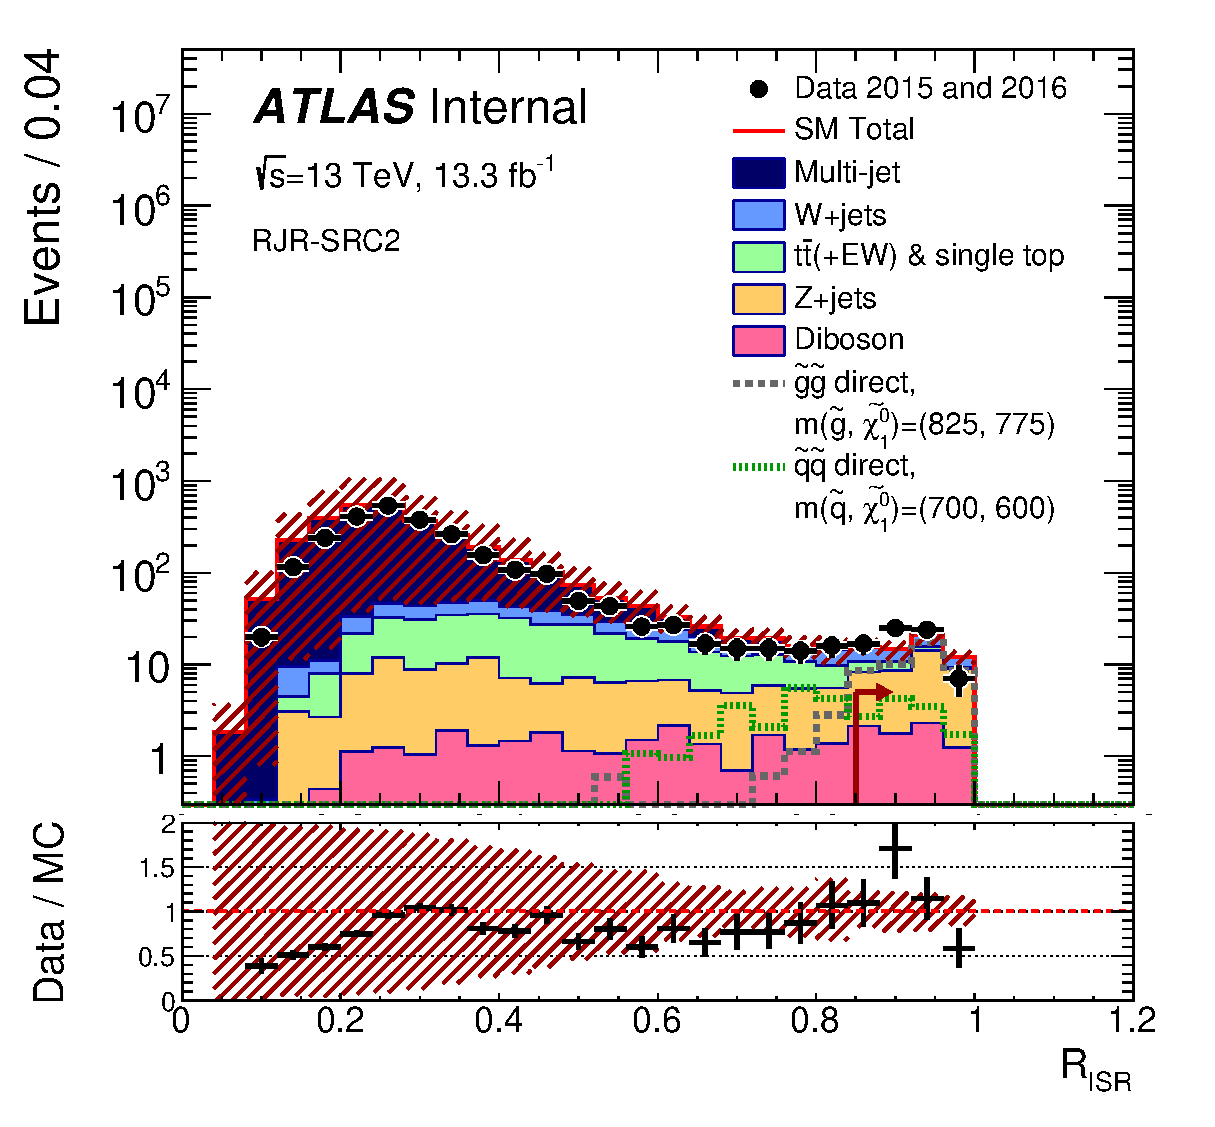
\includegraphics[width=0.33\textwidth]{ATLAS-CONF-2016-078_INT/N-1Plots/AtlasStyle/SR_SRJigsawSRC2_Ratio_SR_minusone}
\end{center}
\caption{}
\label{fig:SR_SRJigsawSRC1_met_SR_minusone}
\end{figure}

\clearpage
\begin{figure}[tbph]
\begin{center}
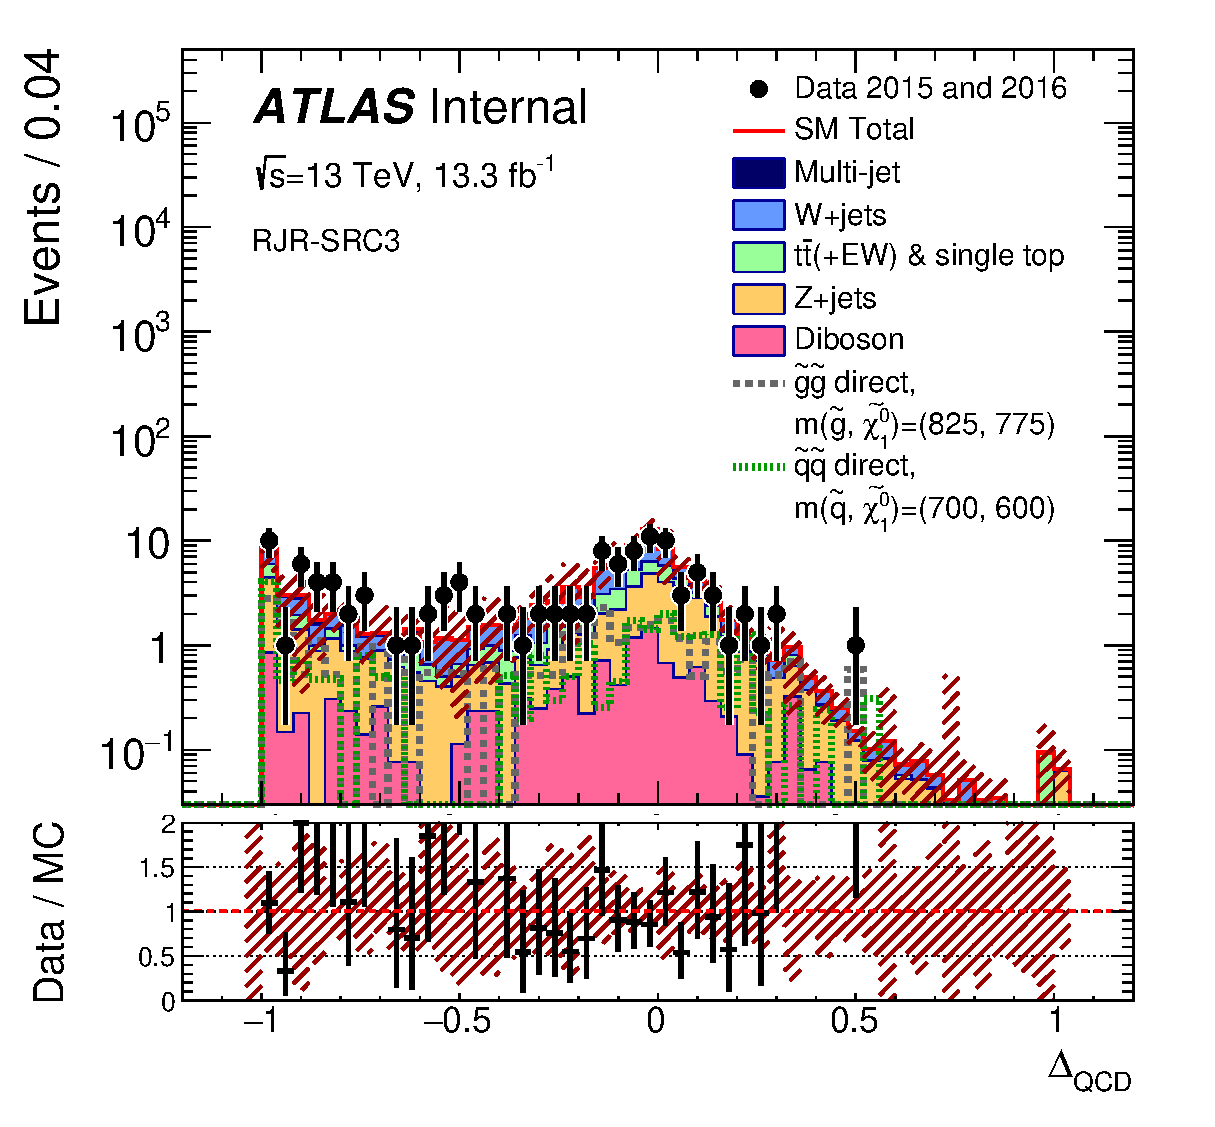
\includegraphics[width=0.33\textwidth]{ATLAS-CONF-2016-078_INT/N-1Plots/AtlasStyle/SR_SRJigsawSRC3_deltaQCD_SR_minusone}
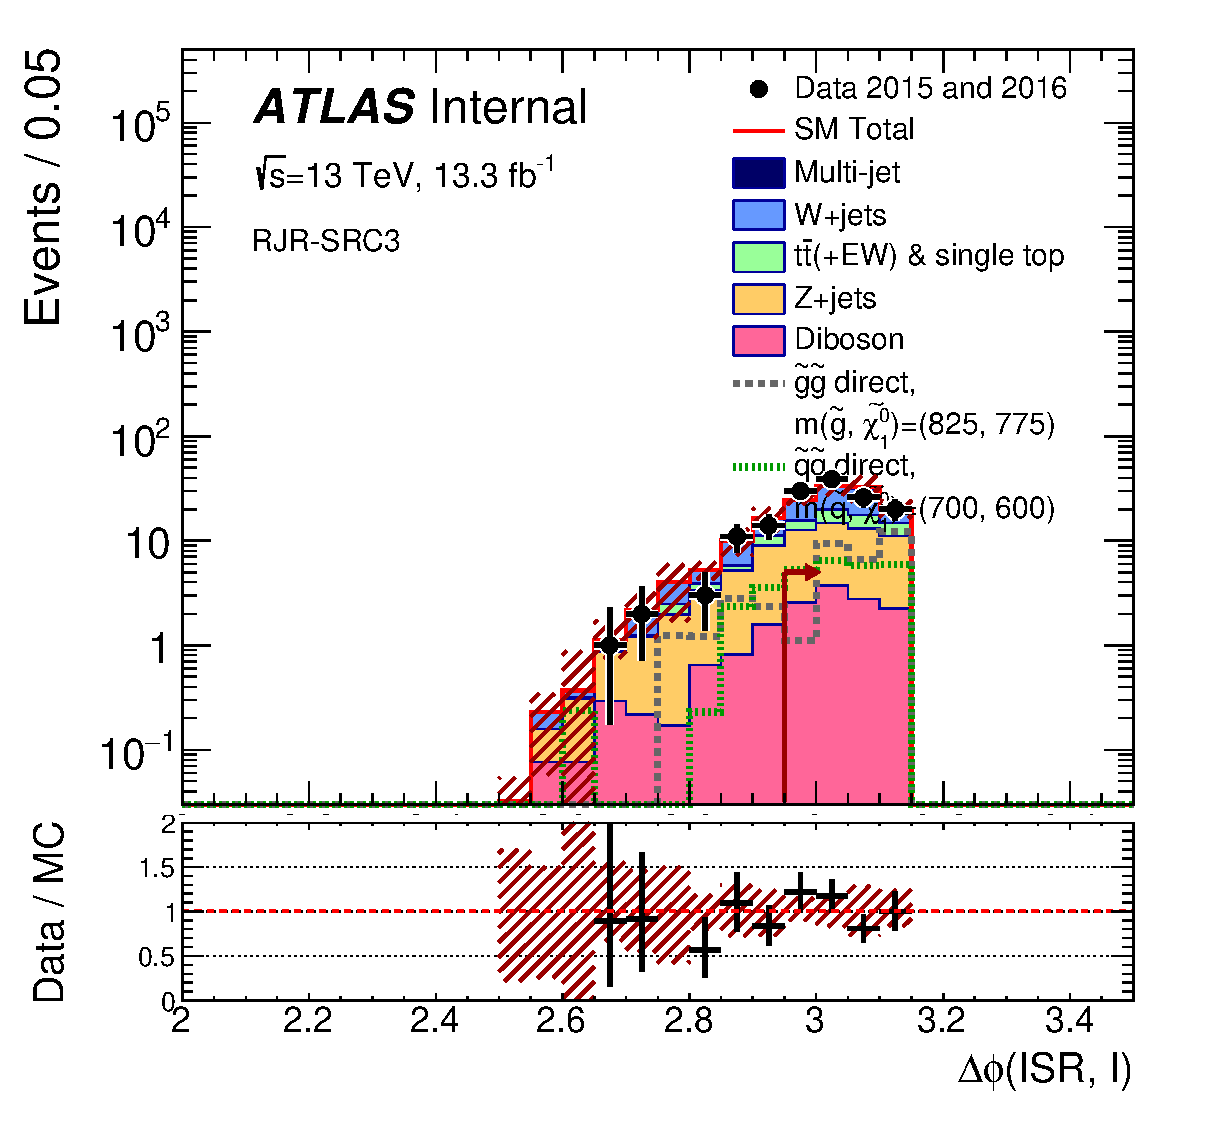
\includegraphics[width=0.33\textwidth]{ATLAS-CONF-2016-078_INT/N-1Plots/AtlasStyle/SR_SRJigsawSRC3_dphiISRI_SR_minusone}
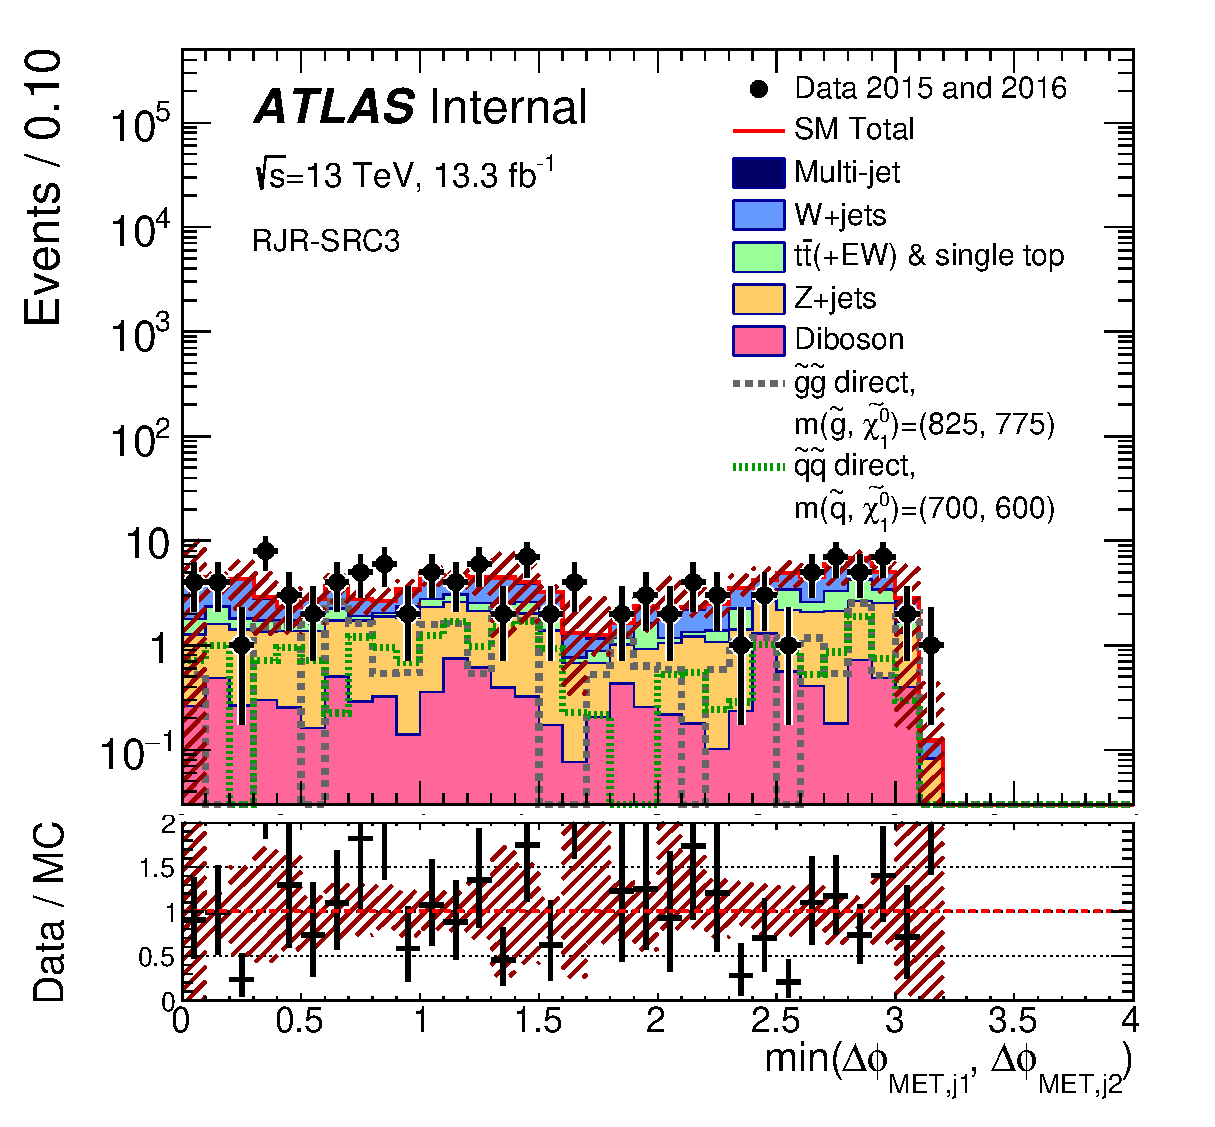
\includegraphics[width=0.33\textwidth]{ATLAS-CONF-2016-078_INT/N-1Plots/AtlasStyle/SR_SRJigsawSRC3_dphiMin2_SR_minusone}
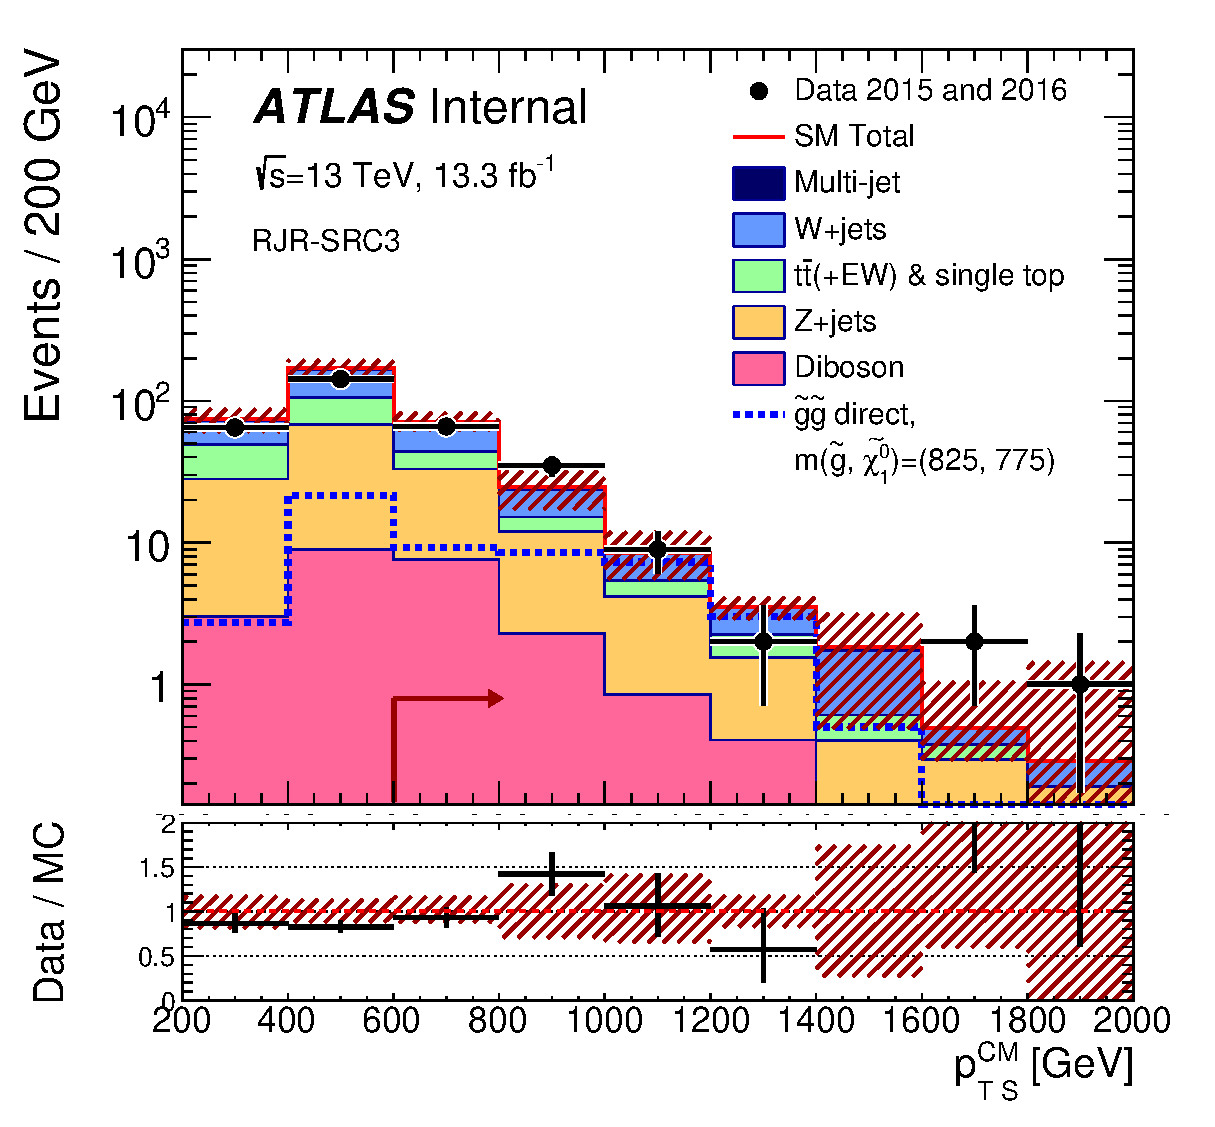
\includegraphics[width=0.33\textwidth]{ATLAS-CONF-2016-078_INT/N-1Plots/AtlasStyle/SR_SRJigsawSRC3_LastCut_SR_minusone}
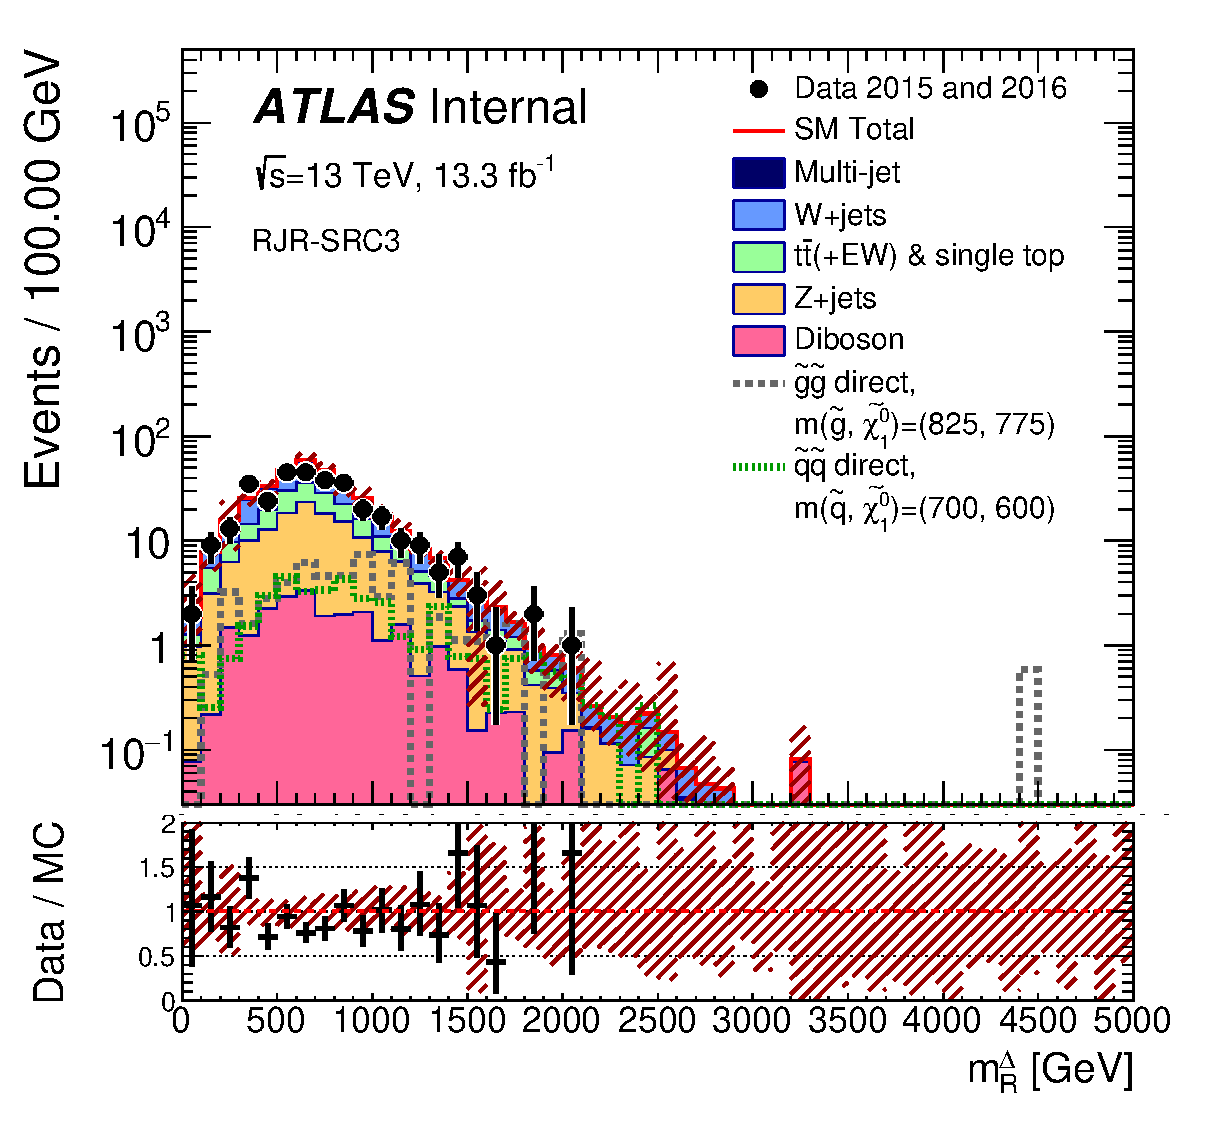
\includegraphics[width=0.33\textwidth]{ATLAS-CONF-2016-078_INT/N-1Plots/AtlasStyle/SR_SRJigsawSRC3_mDR_SR_minusone}
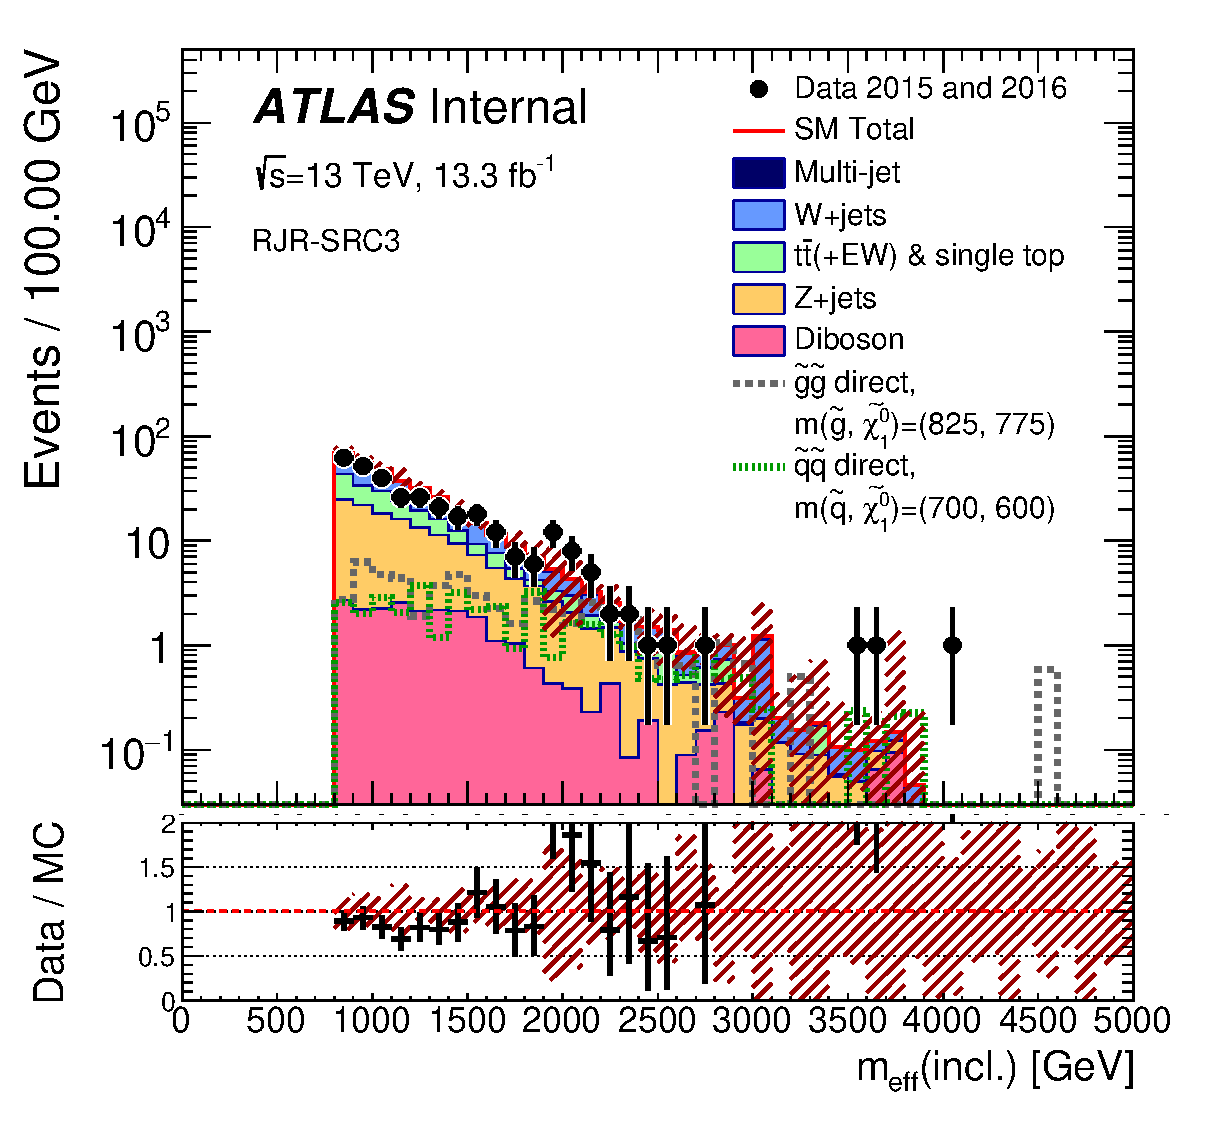
\includegraphics[width=0.33\textwidth]{ATLAS-CONF-2016-078_INT/N-1Plots/AtlasStyle/SR_SRJigsawSRC3_meffincl_SR_minusone}
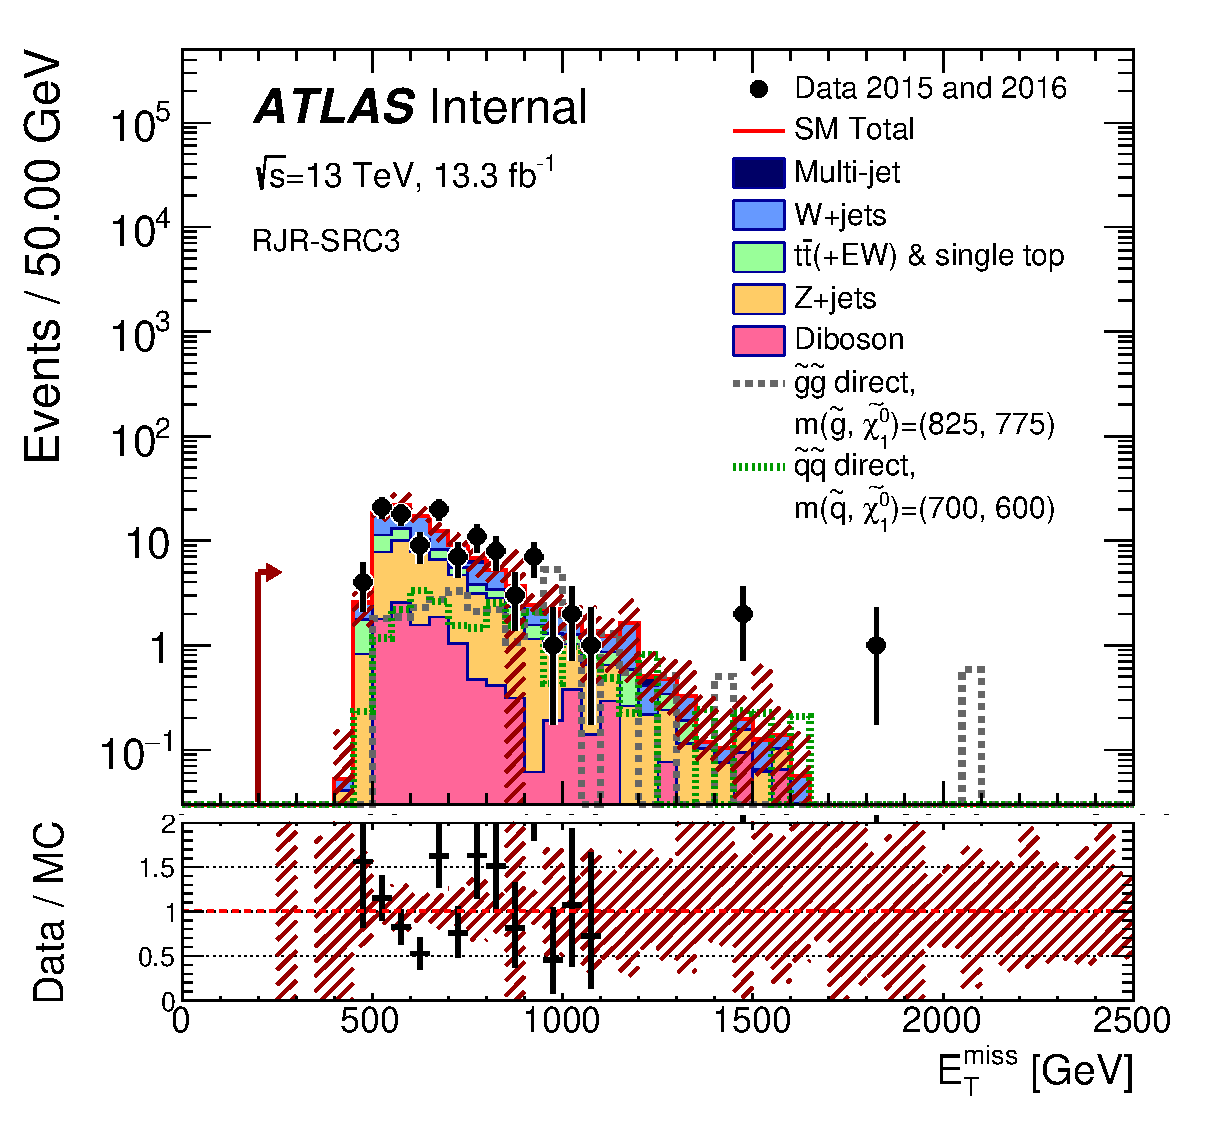
\includegraphics[width=0.33\textwidth]{ATLAS-CONF-2016-078_INT/N-1Plots/AtlasStyle/SR_SRJigsawSRC3_met_SR_minusone}
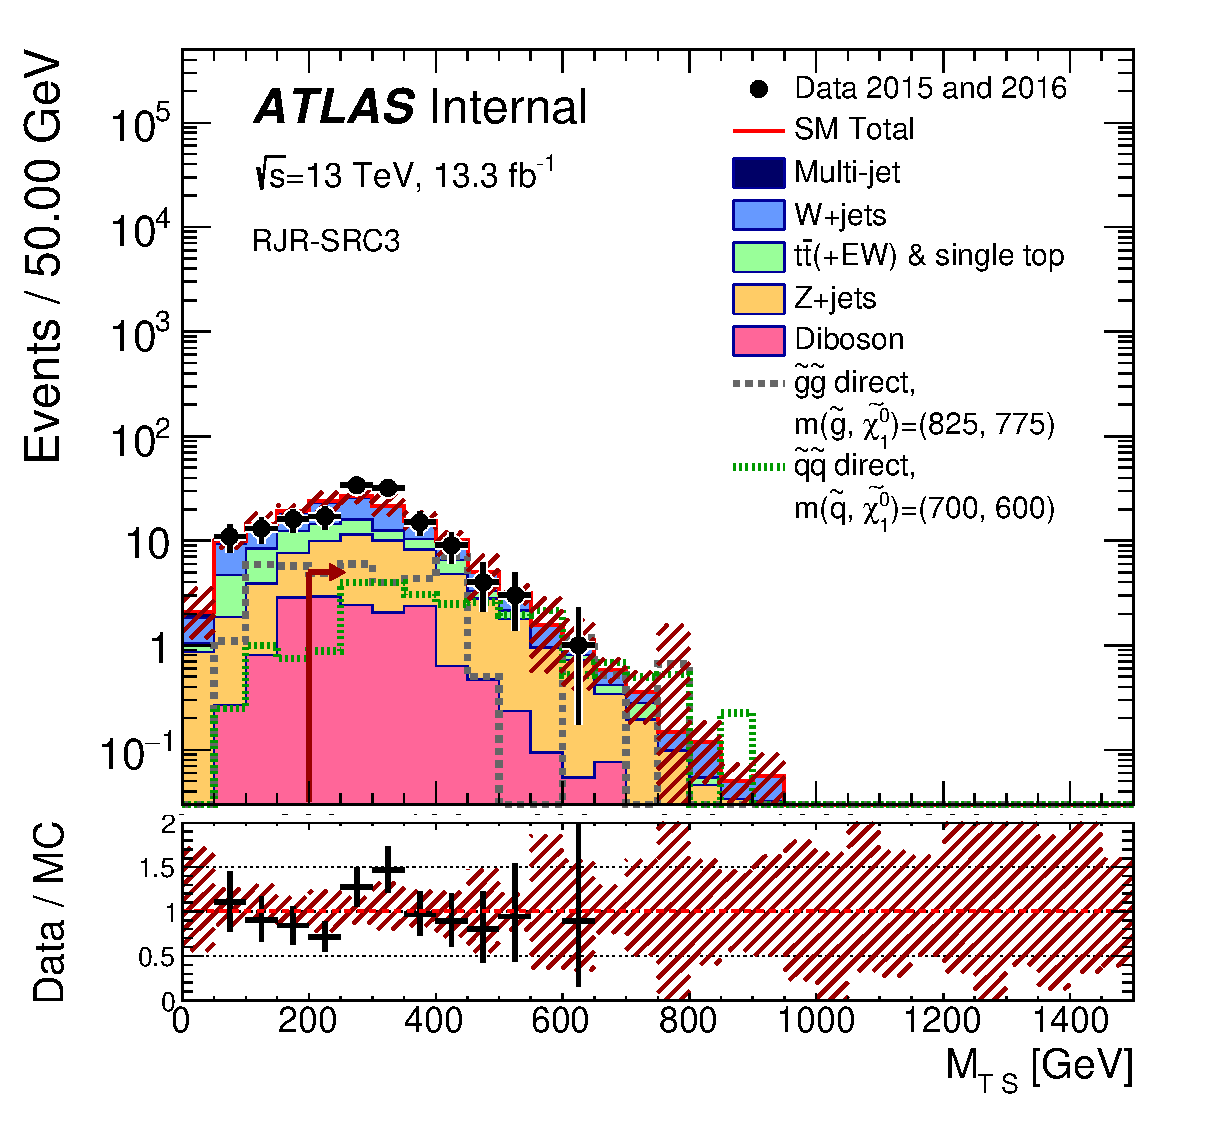
\includegraphics[width=0.33\textwidth]{ATLAS-CONF-2016-078_INT/N-1Plots/AtlasStyle/SR_SRJigsawSRC3_MS_SR_minusone}
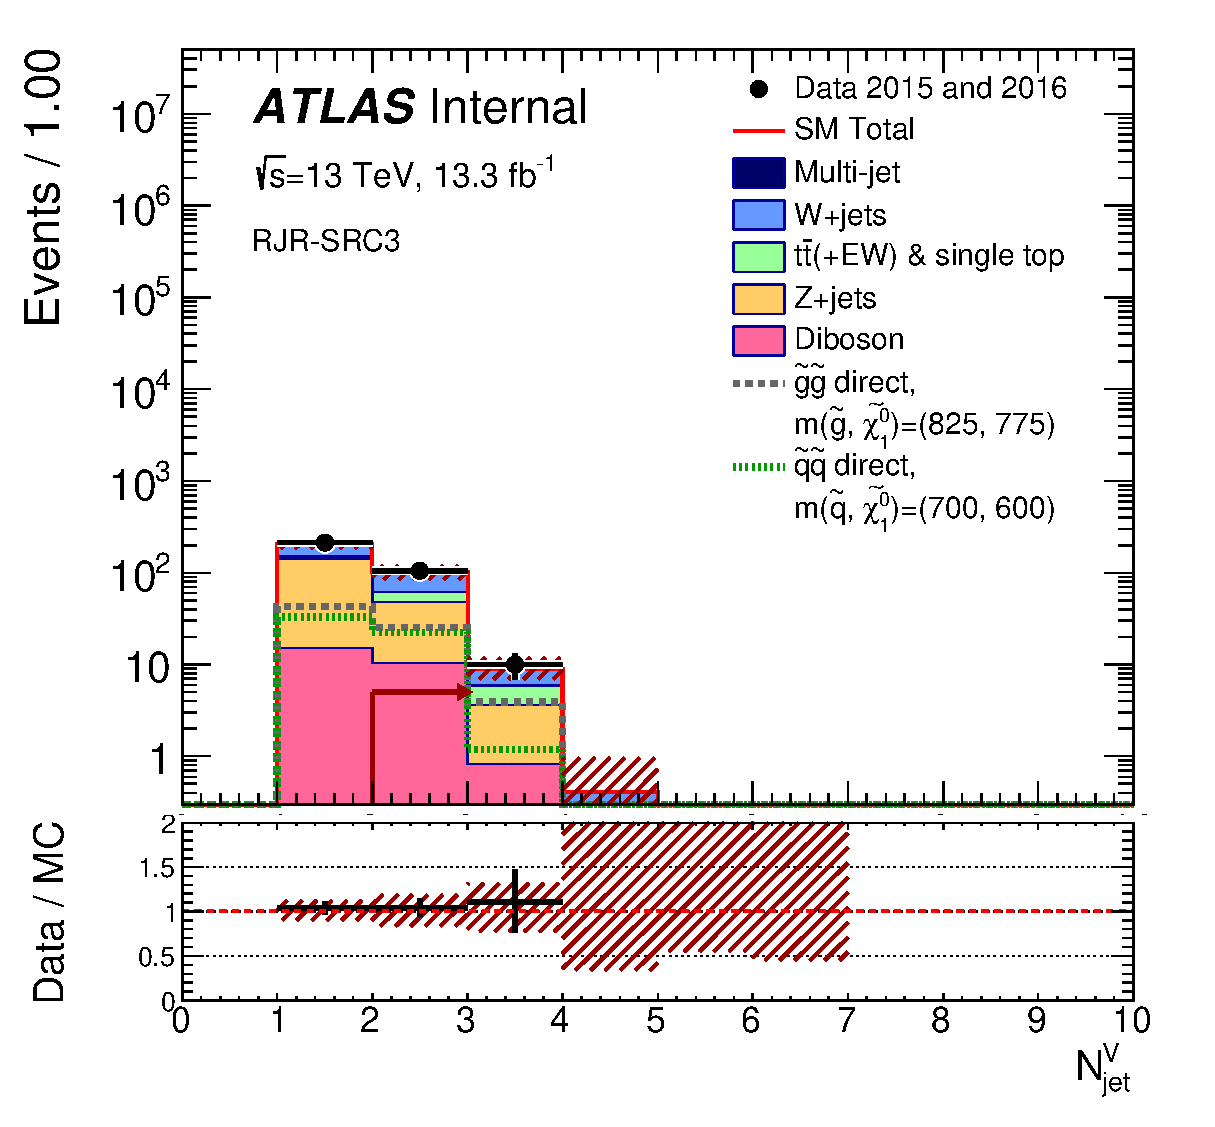
\includegraphics[width=0.33\textwidth]{ATLAS-CONF-2016-078_INT/N-1Plots/AtlasStyle/SR_SRJigsawSRC3_NV_SR_minusone}
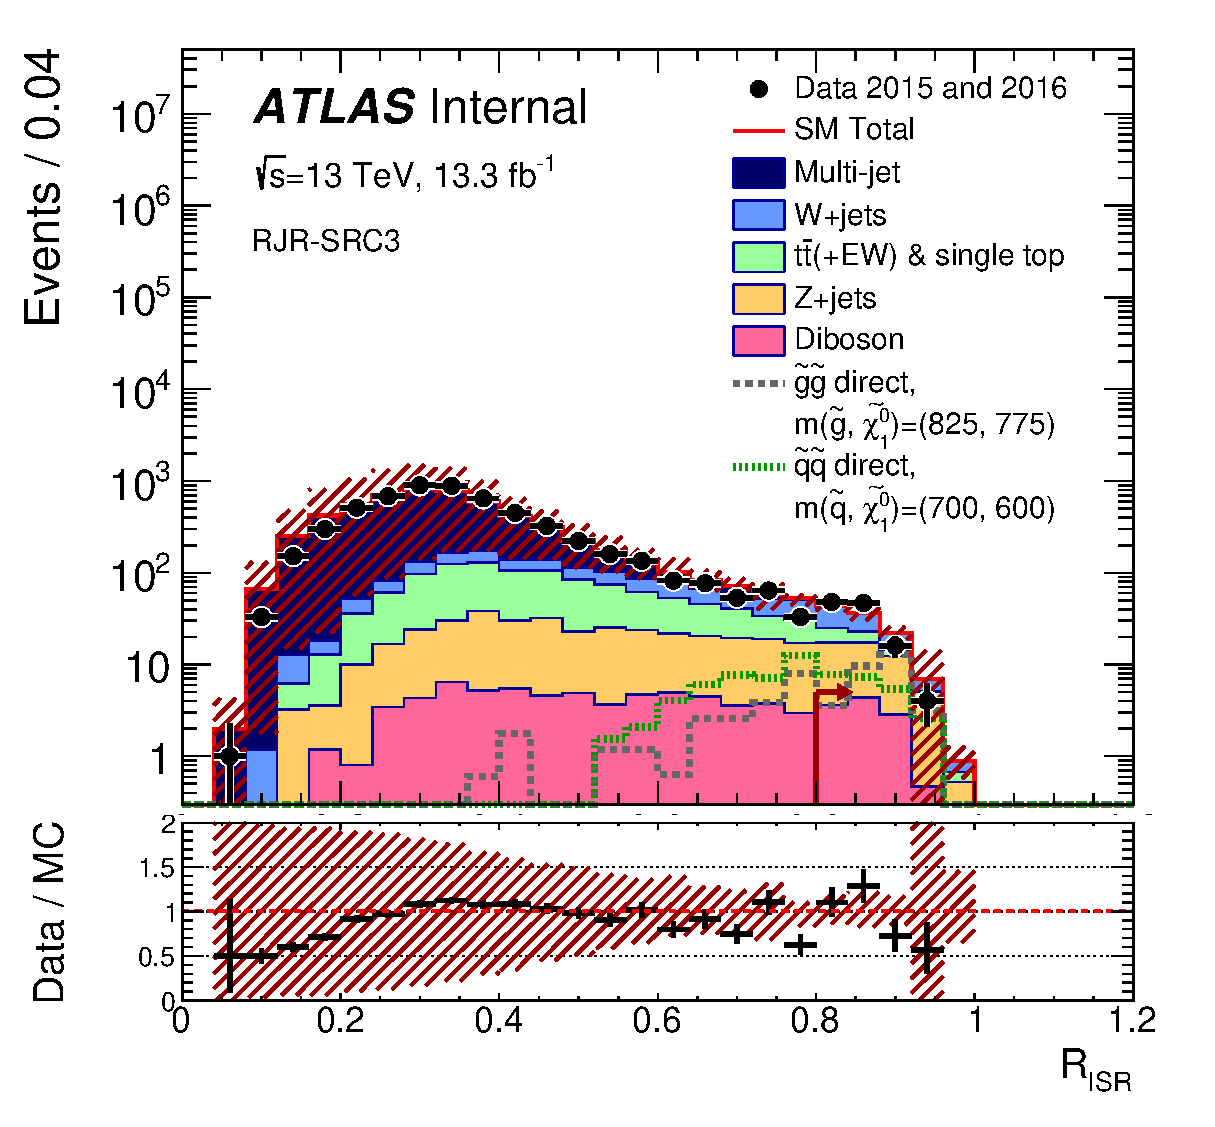
\includegraphics[width=0.33\textwidth]{ATLAS-CONF-2016-078_INT/N-1Plots/AtlasStyle/SR_SRJigsawSRC3_Ratio_SR_minusone}
\end{center}
\caption{}
\label{fig:SR_SRJigsawSRC2_NV_SR_minusone}
\end{figure}

\begin{figure}[tbph]
\begin{center}
\includegraphics[width=0.33\textwidth]{ATLAS-CONF-2016-078_INT/N-1Plots/AtlasStyle/SR_SRJigsawSRC4_deltaQCD_SR_minusone}
\includegraphics[width=0.33\textwidth]{ATLAS-CONF-2016-078_INT/N-1Plots/AtlasStyle/SR_SRJigsawSRC4_dphiISRI_SR_minusone}
\includegraphics[width=0.33\textwidth]{ATLAS-CONF-2016-078_INT/N-1Plots/AtlasStyle/SR_SRJigsawSRC4_dphiMin2_SR_minusone}
\includegraphics[width=0.33\textwidth]{ATLAS-CONF-2016-078_INT/N-1Plots/AtlasStyle/SR_SRJigsawSRC4_LastCut_SR_minusone}
\includegraphics[width=0.33\textwidth]{ATLAS-CONF-2016-078_INT/N-1Plots/AtlasStyle/SR_SRJigsawSRC4_mDR_SR_minusone}
\includegraphics[width=0.33\textwidth]{ATLAS-CONF-2016-078_INT/N-1Plots/AtlasStyle/SR_SRJigsawSRC4_meffincl_SR_minusone}
\includegraphics[width=0.33\textwidth]{ATLAS-CONF-2016-078_INT/N-1Plots/AtlasStyle/SR_SRJigsawSRC4_met_SR_minusone}
\includegraphics[width=0.33\textwidth]{ATLAS-CONF-2016-078_INT/N-1Plots/AtlasStyle/SR_SRJigsawSRC4_MS_SR_minusone}
\includegraphics[width=0.33\textwidth]{ATLAS-CONF-2016-078_INT/N-1Plots/AtlasStyle/SR_SRJigsawSRC4_NV_SR_minusone}
\includegraphics[width=0.33\textwidth]{ATLAS-CONF-2016-078_INT/N-1Plots/AtlasStyle/SR_SRJigsawSRC4_Ratio_SR_minusone}
\end{center}
\caption{}
\label{fig:SR_SRJigsawSRC4_deltaQCD_SR_minusone}
\end{figure}

\clearpage
\begin{figure}[tbph]
\begin{center}
\includegraphics[width=0.33\textwidth]{ATLAS-CONF-2016-078_INT/N-1Plots/AtlasStyle/SR_SRJigsawSRC5_deltaQCD_SR_minusone}
\includegraphics[width=0.33\textwidth]{ATLAS-CONF-2016-078_INT/N-1Plots/AtlasStyle/SR_SRJigsawSRC5_dphiISRI_SR_minusone}
\includegraphics[width=0.33\textwidth]{ATLAS-CONF-2016-078_INT/N-1Plots/AtlasStyle/SR_SRJigsawSRC5_dphiMin2_SR_minusone}
\includegraphics[width=0.33\textwidth]{ATLAS-CONF-2016-078_INT/N-1Plots/AtlasStyle/SR_SRJigsawSRC5_LastCut_SR_minusone}
\includegraphics[width=0.33\textwidth]{ATLAS-CONF-2016-078_INT/N-1Plots/AtlasStyle/SR_SRJigsawSRC5_mDR_SR_minusone}
\includegraphics[width=0.33\textwidth]{ATLAS-CONF-2016-078_INT/N-1Plots/AtlasStyle/SR_SRJigsawSRC5_meffincl_SR_minusone}
\includegraphics[width=0.33\textwidth]{ATLAS-CONF-2016-078_INT/N-1Plots/AtlasStyle/SR_SRJigsawSRC5_met_SR_minusone}
\includegraphics[width=0.33\textwidth]{ATLAS-CONF-2016-078_INT/N-1Plots/AtlasStyle/SR_SRJigsawSRC5_MS_SR_minusone}
\includegraphics[width=0.33\textwidth]{ATLAS-CONF-2016-078_INT/N-1Plots/AtlasStyle/SR_SRJigsawSRC5_NV_SR_minusone}
\includegraphics[width=0.33\textwidth]{ATLAS-CONF-2016-078_INT/N-1Plots/AtlasStyle/SR_SRJigsawSRC5_Ratio_SR_minusone}
\end{center}
\caption{}
\label{fig:SR_SRJigsawSRC5_dphiMin2_SR_minusone}
\end{figure}

\begin{figure}[tbph]
\begin{center}
\includegraphics[width=0.33\textwidth]{ATLAS-CONF-2016-078_INT/N-1Plots/AtlasStyle/SR_SRJigsawSRG1a_dangle_SR_minusone}
\includegraphics[width=0.33\textwidth]{ATLAS-CONF-2016-078_INT/N-1Plots/AtlasStyle/SR_SRJigsawSRG1a_deltaQCD_SR_minusone}
\includegraphics[width=0.33\textwidth]{ATLAS-CONF-2016-078_INT/N-1Plots/AtlasStyle/SR_SRJigsawSRG1a_H2PP_SR_minusone}
\includegraphics[width=0.33\textwidth]{ATLAS-CONF-2016-078_INT/N-1Plots/AtlasStyle/SR_SRJigsawSRG1a_LastCut_SR_minusone}
\includegraphics[width=0.33\textwidth]{ATLAS-CONF-2016-078_INT/N-1Plots/AtlasStyle/SR_SRJigsawSRG1a_maxR_H1PPi_H2PPi_SR_minusone}
\includegraphics[width=0.33\textwidth]{ATLAS-CONF-2016-078_INT/N-1Plots/AtlasStyle/SR_SRJigsawSRG1a_mDR_SR_minusone}
\includegraphics[width=0.33\textwidth]{ATLAS-CONF-2016-078_INT/N-1Plots/AtlasStyle/SR_SRJigsawSRG1a_meffincl_SR_minusone}
\includegraphics[width=0.33\textwidth]{ATLAS-CONF-2016-078_INT/N-1Plots/AtlasStyle/SR_SRJigsawSRG1a_met_SR_minusone}
\includegraphics[width=0.33\textwidth]{ATLAS-CONF-2016-078_INT/N-1Plots/AtlasStyle/SR_SRJigsawSRG1a_minR_pTj2i_HT3PPi_SR_minusone}
\includegraphics[width=0.33\textwidth]{ATLAS-CONF-2016-078_INT/N-1Plots/AtlasStyle/SR_SRJigsawSRG1a_Ratio_SR_minusone}
\includegraphics[width=0.33\textwidth]{ATLAS-CONF-2016-078_INT/N-1Plots/AtlasStyle/SR_SRJigsawSRG1a_RPZ_HT5PP_SR_minusone}
\end{center}
\caption{}
\label{fig:SR_SRJigsawSRG1a_maxR_H1PPi_H2PPi_SR_minusone}
\end{figure}

\begin{figure}[tbph]
\begin{center}
\end{center}
\caption{}
\label{fig:SR_SRJigsawSRG1a_RPZ_HT5PP_SR_minusone}
\end{figure}

\clearpage
\begin{figure}[tbph]
\begin{center}

\includegraphics[width=0.33\textwidth]{ATLAS-CONF-2016-078_INT/N-1Plots/AtlasStyle/SR_SRJigsawSRG1b_dangle_SR_minusone}
\includegraphics[width=0.33\textwidth]{ATLAS-CONF-2016-078_INT/N-1Plots/AtlasStyle/SR_SRJigsawSRG1b_deltaQCD_SR_minusone}
\includegraphics[width=0.33\textwidth]{ATLAS-CONF-2016-078_INT/N-1Plots/AtlasStyle/SR_SRJigsawSRG1b_H2PP_SR_minusone}
\includegraphics[width=0.33\textwidth]{ATLAS-CONF-2016-078_INT/N-1Plots/AtlasStyle/SR_SRJigsawSRG1b_LastCut_SR_minusone}
\includegraphics[width=0.33\textwidth]{ATLAS-CONF-2016-078_INT/N-1Plots/AtlasStyle/SR_SRJigsawSRG1b_maxR_H1PPi_H2PPi_SR_minusone}
\includegraphics[width=0.33\textwidth]{ATLAS-CONF-2016-078_INT/N-1Plots/AtlasStyle/SR_SRJigsawSRG1b_mDR_SR_minusone}
\includegraphics[width=0.33\textwidth]{ATLAS-CONF-2016-078_INT/N-1Plots/AtlasStyle/SR_SRJigsawSRG1b_meffincl_SR_minusone}
\includegraphics[width=0.33\textwidth]{ATLAS-CONF-2016-078_INT/N-1Plots/AtlasStyle/SR_SRJigsawSRG1b_met_SR_minusone}
\includegraphics[width=0.33\textwidth]{ATLAS-CONF-2016-078_INT/N-1Plots/AtlasStyle/SR_SRJigsawSRG1b_minR_pTj2i_HT3PPi_SR_minusone}
\includegraphics[width=0.33\textwidth]{ATLAS-CONF-2016-078_INT/N-1Plots/AtlasStyle/SR_SRJigsawSRG1b_Ratio_SR_minusone}
\includegraphics[width=0.33\textwidth]{ATLAS-CONF-2016-078_INT/N-1Plots/AtlasStyle/SR_SRJigsawSRG1b_RPZ_HT5PP_SR_minusone}
\end{center}
\caption{}
\label{fig:SR_SRJigsawSRG1b_mDR_SR_minusone}
\end{figure}

\begin{figure}[tbph]
\begin{center}
\includegraphics[width=0.33\textwidth]{ATLAS-CONF-2016-078_INT/N-1Plots/AtlasStyle/SR_SRJigsawSRG2a_dangle_SR_minusone}
\includegraphics[width=0.33\textwidth]{ATLAS-CONF-2016-078_INT/N-1Plots/AtlasStyle/SR_SRJigsawSRG2a_deltaQCD_SR_minusone}
\includegraphics[width=0.33\textwidth]{ATLAS-CONF-2016-078_INT/N-1Plots/AtlasStyle/SR_SRJigsawSRG2a_H2PP_SR_minusone}
\includegraphics[width=0.33\textwidth]{ATLAS-CONF-2016-078_INT/N-1Plots/AtlasStyle/SR_SRJigsawSRG2a_LastCut_SR_minusone}
\includegraphics[width=0.33\textwidth]{ATLAS-CONF-2016-078_INT/N-1Plots/AtlasStyle/SR_SRJigsawSRG2a_maxR_H1PPi_H2PPi_SR_minusone}
\includegraphics[width=0.33\textwidth]{ATLAS-CONF-2016-078_INT/N-1Plots/AtlasStyle/SR_SRJigsawSRG2a_mDR_SR_minusone}
\includegraphics[width=0.33\textwidth]{ATLAS-CONF-2016-078_INT/N-1Plots/AtlasStyle/SR_SRJigsawSRG2a_meffincl_SR_minusone}
\includegraphics[width=0.33\textwidth]{ATLAS-CONF-2016-078_INT/N-1Plots/AtlasStyle/SR_SRJigsawSRG2a_met_SR_minusone}
\includegraphics[width=0.33\textwidth]{ATLAS-CONF-2016-078_INT/N-1Plots/AtlasStyle/SR_SRJigsawSRG2a_minR_pTj2i_HT3PPi_SR_minusone}
\includegraphics[width=0.33\textwidth]{ATLAS-CONF-2016-078_INT/N-1Plots/AtlasStyle/SR_SRJigsawSRG2a_Ratio_SR_minusone}
\includegraphics[width=0.33\textwidth]{ATLAS-CONF-2016-078_INT/N-1Plots/AtlasStyle/SR_SRJigsawSRG2a_RPZ_HT5PP_SR_minusone}
\end{center}
\caption{}
\label{fig:SR_SRJigsawSRG2a_dangle_SR_minusone}
\end{figure}

\begin{figure}[tbph]
\begin{center}
\end{center}
\caption{}
\label{fig:SR_SRJigsawSRG2a_meffincl_SR_minusone}
\end{figure}

\begin{figure}[tbph]
\begin{center}
\includegraphics[width=0.33\textwidth]{ATLAS-CONF-2016-078_INT/N-1Plots/AtlasStyle/SR_SRJigsawSRG2b_dangle_SR_minusone}
\includegraphics[width=0.33\textwidth]{ATLAS-CONF-2016-078_INT/N-1Plots/AtlasStyle/SR_SRJigsawSRG2b_deltaQCD_SR_minusone}
\includegraphics[width=0.33\textwidth]{ATLAS-CONF-2016-078_INT/N-1Plots/AtlasStyle/SR_SRJigsawSRG2b_H2PP_SR_minusone}
\includegraphics[width=0.33\textwidth]{ATLAS-CONF-2016-078_INT/N-1Plots/AtlasStyle/SR_SRJigsawSRG2b_LastCut_SR_minusone}
\includegraphics[width=0.33\textwidth]{ATLAS-CONF-2016-078_INT/N-1Plots/AtlasStyle/SR_SRJigsawSRG2b_maxR_H1PPi_H2PPi_SR_minusone}
\includegraphics[width=0.33\textwidth]{ATLAS-CONF-2016-078_INT/N-1Plots/AtlasStyle/SR_SRJigsawSRG2b_mDR_SR_minusone}
\includegraphics[width=0.33\textwidth]{ATLAS-CONF-2016-078_INT/N-1Plots/AtlasStyle/SR_SRJigsawSRG2b_meffincl_SR_minusone}
\includegraphics[width=0.33\textwidth]{ATLAS-CONF-2016-078_INT/N-1Plots/AtlasStyle/SR_SRJigsawSRG2b_met_SR_minusone}
\includegraphics[width=0.33\textwidth]{ATLAS-CONF-2016-078_INT/N-1Plots/AtlasStyle/SR_SRJigsawSRG2b_minR_pTj2i_HT3PPi_SR_minusone}
\includegraphics[width=0.33\textwidth]{ATLAS-CONF-2016-078_INT/N-1Plots/AtlasStyle/SR_SRJigsawSRG2b_Ratio_SR_minusone}
\includegraphics[width=0.33\textwidth]{ATLAS-CONF-2016-078_INT/N-1Plots/AtlasStyle/SR_SRJigsawSRG2b_RPZ_HT5PP_SR_minusone}
\end{center}
\caption{}
\label{fig:SR_SRJigsawSRG2b_deltaQCD_SR_minusone}
\end{figure}

\clearpage
\begin{figure}[tbph]
\begin{center}
\includegraphics[width=0.33\textwidth]{ATLAS-CONF-2016-078_INT/N-1Plots/AtlasStyle/SR_SRJigsawSRG3a_dangle_SR_minusone}
\includegraphics[width=0.33\textwidth]{ATLAS-CONF-2016-078_INT/N-1Plots/AtlasStyle/SR_SRJigsawSRG3a_deltaQCD_SR_minusone}
\includegraphics[width=0.33\textwidth]{ATLAS-CONF-2016-078_INT/N-1Plots/AtlasStyle/SR_SRJigsawSRG3a_H2PP_SR_minusone}
\includegraphics[width=0.33\textwidth]{ATLAS-CONF-2016-078_INT/N-1Plots/AtlasStyle/SR_SRJigsawSRG3a_LastCut_SR_minusone}
\includegraphics[width=0.33\textwidth]{ATLAS-CONF-2016-078_INT/N-1Plots/AtlasStyle/SR_SRJigsawSRG3a_maxR_H1PPi_H2PPi_SR_minusone}
\includegraphics[width=0.33\textwidth]{ATLAS-CONF-2016-078_INT/N-1Plots/AtlasStyle/SR_SRJigsawSRG3a_mDR_SR_minusone}
\includegraphics[width=0.33\textwidth]{ATLAS-CONF-2016-078_INT/N-1Plots/AtlasStyle/SR_SRJigsawSRG3a_meffincl_SR_minusone}
\includegraphics[width=0.33\textwidth]{ATLAS-CONF-2016-078_INT/N-1Plots/AtlasStyle/SR_SRJigsawSRG3a_met_SR_minusone}
\includegraphics[width=0.33\textwidth]{ATLAS-CONF-2016-078_INT/N-1Plots/AtlasStyle/SR_SRJigsawSRG3a_minR_pTj2i_HT3PPi_SR_minusone}
\includegraphics[width=0.33\textwidth]{ATLAS-CONF-2016-078_INT/N-1Plots/AtlasStyle/SR_SRJigsawSRG3a_Ratio_SR_minusone}
\includegraphics[width=0.33\textwidth]{ATLAS-CONF-2016-078_INT/N-1Plots/AtlasStyle/SR_SRJigsawSRG3a_RPZ_HT5PP_SR_minusone}
\end{center}
\caption{}
\label{fig:SR_SRJigsawSRG2b_met_SR_minusone}
\end{figure}

\begin{figure}[tbph]
\begin{center}
\end{center}
\caption{}
\label{fig:SR_SRJigsawSRG3a_H2PP_SR_minusone}
\end{figure}

\begin{figure}[tbph]
\begin{center}
\includegraphics[width=0.33\textwidth]{ATLAS-CONF-2016-078_INT/N-1Plots/AtlasStyle/SR_SRJigsawSRG3b_dangle_SR_minusone}
\includegraphics[width=0.33\textwidth]{ATLAS-CONF-2016-078_INT/N-1Plots/AtlasStyle/SR_SRJigsawSRG3b_deltaQCD_SR_minusone}
\includegraphics[width=0.33\textwidth]{ATLAS-CONF-2016-078_INT/N-1Plots/AtlasStyle/SR_SRJigsawSRG3b_H2PP_SR_minusone}
\includegraphics[width=0.33\textwidth]{ATLAS-CONF-2016-078_INT/N-1Plots/AtlasStyle/SR_SRJigsawSRG3b_LastCut_SR_minusone}
\includegraphics[width=0.33\textwidth]{ATLAS-CONF-2016-078_INT/N-1Plots/AtlasStyle/SR_SRJigsawSRG3b_maxR_H1PPi_H2PPi_SR_minusone}
\includegraphics[width=0.33\textwidth]{ATLAS-CONF-2016-078_INT/N-1Plots/AtlasStyle/SR_SRJigsawSRG3b_mDR_SR_minusone}
\includegraphics[width=0.33\textwidth]{ATLAS-CONF-2016-078_INT/N-1Plots/AtlasStyle/SR_SRJigsawSRG3b_meffincl_SR_minusone}
\includegraphics[width=0.33\textwidth]{ATLAS-CONF-2016-078_INT/N-1Plots/AtlasStyle/SR_SRJigsawSRG3b_met_SR_minusone}
\includegraphics[width=0.33\textwidth]{ATLAS-CONF-2016-078_INT/N-1Plots/AtlasStyle/SR_SRJigsawSRG3b_minR_pTj2i_HT3PPi_SR_minusone}
\includegraphics[width=0.33\textwidth]{ATLAS-CONF-2016-078_INT/N-1Plots/AtlasStyle/SR_SRJigsawSRG3b_Ratio_SR_minusone}
\includegraphics[width=0.33\textwidth]{ATLAS-CONF-2016-078_INT/N-1Plots/AtlasStyle/SR_SRJigsawSRG3b_RPZ_HT5PP_SR_minusone}
\end{center}
\caption{}
\label{fig:SR_SRJigsawSRG3a_minR_pTj2i_HT3PPi_SR_minusone}
\end{figure}

\begin{figure}[tbph]
\begin{center}
\end{center}
\caption{}
\label{fig:SR_SRJigsawSRG3b_LastCut_SR_minusone}
\end{figure}

\clearpage
\begin{figure}[tbph]
\begin{center}
\includegraphics[width=0.33\textwidth]{ATLAS-CONF-2016-078_INT/N-1Plots/AtlasStyle/SR_SRJigsawSRS1a_deltaQCD_SR_minusone}
\includegraphics[width=0.33\textwidth]{ATLAS-CONF-2016-078_INT/N-1Plots/AtlasStyle/SR_SRJigsawSRS1a_H2PP_SR_minusone}
\includegraphics[width=0.33\textwidth]{ATLAS-CONF-2016-078_INT/N-1Plots/AtlasStyle/SR_SRJigsawSRS1a_LastCut_SR_minusone}
\includegraphics[width=0.33\textwidth]{ATLAS-CONF-2016-078_INT/N-1Plots/AtlasStyle/SR_SRJigsawSRS1a_mDR_SR_minusone}
\includegraphics[width=0.33\textwidth]{ATLAS-CONF-2016-078_INT/N-1Plots/AtlasStyle/SR_SRJigsawSRS1a_meffincl_SR_minusone}
\includegraphics[width=0.33\textwidth]{ATLAS-CONF-2016-078_INT/N-1Plots/AtlasStyle/SR_SRJigsawSRS1a_met_SR_minusone}
\includegraphics[width=0.33\textwidth]{ATLAS-CONF-2016-078_INT/N-1Plots/AtlasStyle/SR_SRJigsawSRS1a_R_pTj2_HT3PP_SR_minusone}
\includegraphics[width=0.33\textwidth]{ATLAS-CONF-2016-078_INT/N-1Plots/AtlasStyle/SR_SRJigsawSRS1a_Ratio_SR_minusone}
\includegraphics[width=0.33\textwidth]{ATLAS-CONF-2016-078_INT/N-1Plots/AtlasStyle/SR_SRJigsawSRS1a_RPZ_HT3PP_SR_minusone}
\end{center}
\caption{}
\label{fig:SR_SRJigsawSRG3b_Ratio_SR_minusone}
\end{figure}

\begin{figure}[tbph]
\begin{center}
\end{center}
\caption{}
\label{fig:SR_SRJigsawSRS1a_meffincl_SR_minusone}
\end{figure}

\begin{figure}[tbph]
\begin{center}
\includegraphics[width=0.33\textwidth]{ATLAS-CONF-2016-078_INT/N-1Plots/AtlasStyle/SR_SRJigsawSRS1b_deltaQCD_SR_minusone}
\includegraphics[width=0.33\textwidth]{ATLAS-CONF-2016-078_INT/N-1Plots/AtlasStyle/SR_SRJigsawSRS1b_H2PP_SR_minusone}
\includegraphics[width=0.33\textwidth]{ATLAS-CONF-2016-078_INT/N-1Plots/AtlasStyle/SR_SRJigsawSRS1b_LastCut_SR_minusone}
\includegraphics[width=0.33\textwidth]{ATLAS-CONF-2016-078_INT/N-1Plots/AtlasStyle/SR_SRJigsawSRS1b_mDR_SR_minusone}
\includegraphics[width=0.33\textwidth]{ATLAS-CONF-2016-078_INT/N-1Plots/AtlasStyle/SR_SRJigsawSRS1b_meffincl_SR_minusone}
\includegraphics[width=0.33\textwidth]{ATLAS-CONF-2016-078_INT/N-1Plots/AtlasStyle/SR_SRJigsawSRS1b_met_SR_minusone}
\includegraphics[width=0.33\textwidth]{ATLAS-CONF-2016-078_INT/N-1Plots/AtlasStyle/SR_SRJigsawSRS1b_R_pTj2_HT3PP_SR_minusone}
\includegraphics[width=0.33\textwidth]{ATLAS-CONF-2016-078_INT/N-1Plots/AtlasStyle/SR_SRJigsawSRS1b_Ratio_SR_minusone}
\includegraphics[width=0.33\textwidth]{ATLAS-CONF-2016-078_INT/N-1Plots/AtlasStyle/SR_SRJigsawSRS1b_RPZ_HT3PP_SR_minusone}
\end{center}
\caption{}
\label{fig:SR_SRJigsawSRS1b_H2PP_SR_minusone}
\end{figure}

\begin{figure}[tbph]
\begin{center}
\includegraphics[width=0.33\textwidth]{ATLAS-CONF-2016-078_INT/N-1Plots/AtlasStyle/SR_SRJigsawSRS2a_deltaQCD_SR_minusone}
\includegraphics[width=0.33\textwidth]{ATLAS-CONF-2016-078_INT/N-1Plots/AtlasStyle/SR_SRJigsawSRS2a_H2PP_SR_minusone}
\includegraphics[width=0.33\textwidth]{ATLAS-CONF-2016-078_INT/N-1Plots/AtlasStyle/SR_SRJigsawSRS2a_LastCut_SR_minusone}
\includegraphics[width=0.33\textwidth]{ATLAS-CONF-2016-078_INT/N-1Plots/AtlasStyle/SR_SRJigsawSRS2a_mDR_SR_minusone}
\includegraphics[width=0.33\textwidth]{ATLAS-CONF-2016-078_INT/N-1Plots/AtlasStyle/SR_SRJigsawSRS2a_meffincl_SR_minusone}
\includegraphics[width=0.33\textwidth]{ATLAS-CONF-2016-078_INT/N-1Plots/AtlasStyle/SR_SRJigsawSRS2a_met_SR_minusone}
\includegraphics[width=0.33\textwidth]{ATLAS-CONF-2016-078_INT/N-1Plots/AtlasStyle/SR_SRJigsawSRS2a_R_pTj2_HT3PP_SR_minusone}
\includegraphics[width=0.33\textwidth]{ATLAS-CONF-2016-078_INT/N-1Plots/AtlasStyle/SR_SRJigsawSRS2a_Ratio_SR_minusone}
\includegraphics[width=0.33\textwidth]{ATLAS-CONF-2016-078_INT/N-1Plots/AtlasStyle/SR_SRJigsawSRS2a_RPZ_HT3PP_SR_minusone}
\end{center}
\caption{}
\label{fig:SR_SRJigsawSRS1b_Ratio_SR_minusone}
\end{figure}

\clearpage
\begin{figure}[tbph]
\begin{center}
\includegraphics[width=0.33\textwidth]{ATLAS-CONF-2016-078_INT/N-1Plots/AtlasStyle/SR_SRJigsawSRS2b_deltaQCD_SR_minusone}
\includegraphics[width=0.33\textwidth]{ATLAS-CONF-2016-078_INT/N-1Plots/AtlasStyle/SR_SRJigsawSRS2b_H2PP_SR_minusone}
\includegraphics[width=0.33\textwidth]{ATLAS-CONF-2016-078_INT/N-1Plots/AtlasStyle/SR_SRJigsawSRS2b_LastCut_SR_minusone}
\includegraphics[width=0.33\textwidth]{ATLAS-CONF-2016-078_INT/N-1Plots/AtlasStyle/SR_SRJigsawSRS2b_mDR_SR_minusone}
\includegraphics[width=0.33\textwidth]{ATLAS-CONF-2016-078_INT/N-1Plots/AtlasStyle/SR_SRJigsawSRS2b_meffincl_SR_minusone}
\includegraphics[width=0.33\textwidth]{ATLAS-CONF-2016-078_INT/N-1Plots/AtlasStyle/SR_SRJigsawSRS2b_met_SR_minusone}
\includegraphics[width=0.33\textwidth]{ATLAS-CONF-2016-078_INT/N-1Plots/AtlasStyle/SR_SRJigsawSRS2b_R_pTj2_HT3PP_SR_minusone}
\includegraphics[width=0.33\textwidth]{ATLAS-CONF-2016-078_INT/N-1Plots/AtlasStyle/SR_SRJigsawSRS2b_Ratio_SR_minusone}
\includegraphics[width=0.33\textwidth]{ATLAS-CONF-2016-078_INT/N-1Plots/AtlasStyle/SR_SRJigsawSRS2b_RPZ_HT3PP_SR_minusone}
\end{center}
\caption{}
\label{fig:SR_SRJigsawSRS2a_meffincl_SR_minusone}
\end{figure}

\begin{figure}[tbph]
\begin{center}
\includegraphics[width=0.33\textwidth]{ATLAS-CONF-2016-078_INT/N-1Plots/AtlasStyle/SR_SRJigsawSRS3a_deltaQCD_SR_minusone}
\includegraphics[width=0.33\textwidth]{ATLAS-CONF-2016-078_INT/N-1Plots/AtlasStyle/SR_SRJigsawSRS3a_H2PP_SR_minusone}
\includegraphics[width=0.33\textwidth]{ATLAS-CONF-2016-078_INT/N-1Plots/AtlasStyle/SR_SRJigsawSRS3a_LastCut_SR_minusone}
\includegraphics[width=0.33\textwidth]{ATLAS-CONF-2016-078_INT/N-1Plots/AtlasStyle/SR_SRJigsawSRS3a_mDR_SR_minusone}
\includegraphics[width=0.33\textwidth]{ATLAS-CONF-2016-078_INT/N-1Plots/AtlasStyle/SR_SRJigsawSRS3a_meffincl_SR_minusone}
\includegraphics[width=0.33\textwidth]{ATLAS-CONF-2016-078_INT/N-1Plots/AtlasStyle/SR_SRJigsawSRS3a_met_SR_minusone}
\includegraphics[width=0.33\textwidth]{ATLAS-CONF-2016-078_INT/N-1Plots/AtlasStyle/SR_SRJigsawSRS3a_R_pTj2_HT3PP_SR_minusone}
\includegraphics[width=0.33\textwidth]{ATLAS-CONF-2016-078_INT/N-1Plots/AtlasStyle/SR_SRJigsawSRS3a_Ratio_SR_minusone}
\includegraphics[width=0.33\textwidth]{ATLAS-CONF-2016-078_INT/N-1Plots/AtlasStyle/SR_SRJigsawSRS3a_RPZ_HT3PP_SR_minusone}
\end{center}
\caption{}
\label{fig:SR_SRJigsawSRS2b_H2PP_SR_minusone}
\end{figure}

\begin{figure}[tbph]
\begin{center}
\includegraphics[width=0.33\textwidth]{ATLAS-CONF-2016-078_INT/N-1Plots/AtlasStyle/SR_SRJigsawSRS3b_deltaQCD_SR_minusone}
\includegraphics[width=0.33\textwidth]{ATLAS-CONF-2016-078_INT/N-1Plots/AtlasStyle/SR_SRJigsawSRS3b_H2PP_SR_minusone}
\includegraphics[width=0.33\textwidth]{ATLAS-CONF-2016-078_INT/N-1Plots/AtlasStyle/SR_SRJigsawSRS3b_LastCut_SR_minusone}
\includegraphics[width=0.33\textwidth]{ATLAS-CONF-2016-078_INT/N-1Plots/AtlasStyle/SR_SRJigsawSRS3b_mDR_SR_minusone}
\includegraphics[width=0.33\textwidth]{ATLAS-CONF-2016-078_INT/N-1Plots/AtlasStyle/SR_SRJigsawSRS3b_meffincl_SR_minusone}
\includegraphics[width=0.33\textwidth]{ATLAS-CONF-2016-078_INT/N-1Plots/AtlasStyle/SR_SRJigsawSRS3b_met_SR_minusone}
\includegraphics[width=0.33\textwidth]{ATLAS-CONF-2016-078_INT/N-1Plots/AtlasStyle/SR_SRJigsawSRS3b_R_pTj2_HT3PP_SR_minusone}
\includegraphics[width=0.33\textwidth]{ATLAS-CONF-2016-078_INT/N-1Plots/AtlasStyle/SR_SRJigsawSRS3b_Ratio_SR_minusone}
\includegraphics[width=0.33\textwidth]{ATLAS-CONF-2016-078_INT/N-1Plots/AtlasStyle/SR_SRJigsawSRS3b_RPZ_HT3PP_SR_minusone}
\end{center}
\caption{}
\label{fig:SR_SRJigsawSRS3a_meffincl_SR_minusone}
\end{figure}

\clearpage



\end{document} %All done! Now you're a doctor.
